\chapter{System design and implementation}
\label{cha:design}

This chapter presents the design and implementation of our system, focusing on the integration of the various components and the overall architecture. 
A general description of some of the key components is provided to better explain their role in the system and the reasons for their inclusion.
The system is designed to be modular, scalable, and extensible, enabling the integration of additional components as needed.
It must be said the the following is a description of a first iteration of the system. 

\section{Assumptions}

In this section we present the assumptions made during the design and implementation of the system. 

\subsection{Workload definition}
In this work, workloads has been modeled as \textbf{Virtual Machines (VMs)}, representing the \textbf{primary use case} considered during the system's initial design phase. 
It is possible to define as ``interrupible workloads", those workloads that can be stopped and restarted without losing the work done. 
For this first iteration of the system only ``\textbf{non-interruptible workloads}" are considered.
This choice was driven by the fact the Virtual Machines are both a common and widely used cloud resource and one of the simplest to provision on multiple cloud providers and therefore ideal for the first iteration of the system.
Having said that, for the purpose of this work, a simple formalization can be done.

A VM is defined as a tuple:

\[
\text{VM} = (\text{MinCPU}, \text{MinRAM}, D, DL, ML)
\]

where:
\begin{itemize}[itemsep=0.2pt, topsep=1pt]
    \item \( \text{MinCPU} \) is the minimum number of virtual CPUs required.
    \item \( \text{MinRAM} \) is the minimum RAM required (in GB).
    \item \( D \) is the duration for which the VM must run to complete its processing task \( P \) (in hours).
    \item \( DL \) is the deadline timestamp by which the VM must complete execution.
    \item \( ML \) is the maximum allowed latency in milliseconds. If latency is not a constraint, then a high value can be set (e.g., \( ML = 2000 \)). \\
\end{itemize}

This VM can be scheduled on any Public Cloud Provider since we are interested in a multi-cloud system where the cloud can be effectively seen as a commodity. 
Alternatively, a subset of \textbf{eligible Public Cloud Providers} can be set at runtime by the user.
We will refer to \textbf{general-purpose VMs} and not specialized ones like GPU instances or high-performance computing instances. \\

As an example, we can define a VM with the following specifications:

\[
\text{VM}_{\text{example}} = (4, 4, 2, \texttt{"2025-03-20T23:59:59Z"}, 100)
\]


where:
\begin{itemize}[itemsep=0.2pt, topsep=1pt]
    \item \( \text{MinCPU} = 4 \) vCPUs
    \item \( \text{MinRAM} = 4 \) GB
    \item \( D = 1 \) hour
    \item \( DL = \texttt{"2025-03-20T23:59:59Z"} \) (i.e., the processing task \( P \) inside the VM must complete before this timestamp) \\
\end{itemize}

The system is designed to be cloud-agnostic, however for the purpose of this work, the system is currently configured to support three major cloud providers: \textbf{Microsoft Azure}, \textbf{Google Cloud Platform (GCP)}, and \textbf{Amazon Web Services (AWS)}.

\subsection{System limitations}

A limitation of our general approach is that only resources supported by the cloud provider’s Kubernetes operator can be provisioned in a 
seamless way.
Not all cloud resources available in a provider’s portfolio are guaranteed to have corresponding Kubernetes Custom Resources (CRs). This introduces certain constraints:

\begin{itemize}[itemsep=0.2pt, topsep=1pt]
  \item[$\bullet$] Limited resource availability: if a specific resource type (e.g., a GPU-accelerated instance or a database service) is not supported by the cloud provider Operator, it cannot be provisioned using the current system.
  \item[$\bullet$] Dependence on Operator updates: cloud providers may extend or modify the set of resources supported by their Kubernetes operators over time.
  \item[$\bullet$] Vendor-specific implementations: for the same class of resources (e.g., virtual machines), the structure and fields of the CRs may vary a lot between cloud providers.
\end{itemize}

Despite these constraints, the system architecture remains highly adaptable, and future enhancements could incorporate additional or alternative provisioning mechanisms. 
An example of an alternative implementation could be the \textbf{direct API interactions} with cloud providers to bypass operator limitations. As a matter of fact, usually cloud provider Operators are leveraging these APIs under the hood to interact with the cloud provider’s services.
Another approach could involve the development of custom operators or controllers to manage specific resource types not supported by existing operators.
For instance, Krateo PlatformOps provides the so-called ``oasgen-provider'' that aims to fill the gaps of missing or incomplete Kubernetes operators. This module is a Kubernetes controller that is able to generate Kubernetes CRDs and the related controllers from OpenAPI specifications \cite{krateo_oasgen_provider}. 

\newpage

\section{System Architecture}
\label{sec:system_architecture}

The following table provides an overview of the main components of the system and their respective functions.

\begin{table}[H]
  \centering
  \renewcommand{\arraystretch}{1.3} % Adjust row height for readability
  \begin{tabularx}{\textwidth}{| l | X |} % 'X' makes the second column auto-wrap
    \hline
    \textbf{Component} & \textbf{Function} \\
    \hline
    Krateo PlatformOps & Provides an abstraction layer for infrastructure orchestration, enabling declarative resource management and integration with cloud providers with templates. \\
    \hline
    Cloud Providers Kubernetes Operators & Manages the provisioning and reconciliation of cloud resources within Kubernetes, ensuring the actual state matches the desired state. \\
    \hline
    Kubernetes Mutating Webhook Configuration & Intercepts and modifies API requests before they are persisted, allowing dynamic configuration adjustments with policy enforcement. \\
    \hline
    OPA Server & Evaluates policy decisions based on defined constraints and input data from Kubernetes API requests through the webhook configuration. \\
    \hline
    OPA Policies and Data & Define the rules and contextual information used by OPA to make policy decisions, namely scheduling information \\
    \hline
    GreenOps Scheduler & Determines the optimal scheduling region and scheduling time for VMs, acting as an external data source for OPA policies. \\
    \hline
    MLflow & Allows the tracking, logging, versioning and storing of machine learning experiments for reproducibility and model lifecycle management. \\
    \hline
    KServe & Provides scalable and Kubernetes-native model serving capabilities, enabling deployment of machine learning models for inference. \\
    \hline
  \end{tabularx}
  \caption{Main components of the system and their respective functions.}
  \label{tab:system_components}
\end{table}

All the components listed in the above table must be deployed inside a Kubernetes cluster. The only exception are the OPA Policies and data which lies outside the cluster as described in section \ref{sec:opa_bundles}.

\section{Krateo PlatformOps integration}
\label{sec:krateo_integration}

Krateo PlatformOps is leveraged in this system as a core component for \textbf{multi-cloud resource management}, as it allows declarative orchestration of cloud resources across different cloud providers leveraging Kubernetes as a control plane. 
This section highlights the differences between two different approaches that were considered for multi-cloud resource management:
\begin{itemize}[itemsep=0.2pt, topsep=1pt]
  \item[$\bullet$] The \textbf{Custom Kubernetes ``Synchronization Operator"} approach (initially considered)
  \item[$\bullet$] The \textbf{Krateo PlatformOps} approach (adopted in the final system design) \\
\end{itemize}

It is deemed interesting to describe both approaches in order to identify the several \textbf{trade-offs} between implementing a custom Kubernetes ``Synchronization Operator" and leveraging a template-based abstraction for cloud resource provisioning.

\subsection{Resource management: the Custom Kubernetes ``Synchronization Operator" approach}

When dealing with multi-cloud resource management with Kubernetes as a control plane, a \textbf{synchronization and mapping mechanism} (broker) is required to bridge the gap between:
\begin{itemize}[itemsep=0.2pt, topsep=1pt]
  \item[$\bullet$] \textbf{Generic Kubernetes Custom Resources}, which represent generic provider-agnostic workloads.
  \item[$\bullet$] \textbf{Cloud provider-specific Custom Resources}, which correspond to the actual cloud resources provisioned through the respective Kubernetes operators provided by Azure, AWS or GCP (in our case).
\end{itemize}
This requirement was also highlighted in the literature review described in section \ref{sec:multi_cloud_resource_management_components}.

In this first approach, a custom Kubernetes ``Synchronization Operator" would be responsible for the mapping and synchronization of the above resource types. 
Figure \ref{fig:k8s_operator} illustrates the high-level architecture of the system with the custom operator approach.
This approach is based on the principle of \textbf{Continuous Reconciliation}, where the operator continuously monitors and adjusts the system to maintain consistency between the desired and actual states.
Candidate solutions for the implementation of a Kubernetes Operator includes: Operator SDK, Kubebuilder, or writing the operator from scratch using the Kubernetes client libraries. 
For the purpose of this work, Kubebuilder was used to develop a Proof of Concept (PoC) for the custom operator.

\subsubsection{Responsibilities of the ``Synchronization Operator"}

In our specific case, the operator should continuously watch the generic CRs in the Kubernetes cluster to check if critical scheduling fields have been set, in particular:
\begin{itemize}[itemsep=0.2pt, topsep=1pt]
  \item[$\bullet$] \textbf{schedulingRegion}: Defines where the workload should be placed.
  \item[$\bullet$] \textbf{schedulingTime}: Specifies when the workload should be deployed.
\end{itemize}

These fields, if set, indicate a geographical placement and timing for the workload have been determined by the GreenOps Scheduler.
If these fields are not yet present, the operator must wait for scheduling decisions before proceeding.
Therefore, inside its ``\textit{Reconcile()}'' loop, the operator should:
\begin{enumerate}[itemsep=0.2pt, topsep=1pt]
  \item Continuously check if scheduling fields (schedulingRegion, schedulingTime) are set.
  \item Trigger the creation of the provider-specific resource when the schedulingTime is approaching.
  \item Track the provisioning status by marking the generic CR with a field indicating that the cloud-specific resource has been created.
\end{enumerate}

\subsubsection{Post-Creation Considerations}

Once the cloud provider-specific resource is created, two main questions arise:
\begin{itemize}[itemsep=0.2pt, topsep=1pt]
  \item[$\bullet$] What happens if the provider-specific CR is modified manually?
  \item[$\bullet$] What happens if the provider-specific configuration is modified directly on the cloud provider (outside Kubernetes)?
\end{itemize}

Related to the first question, an example scenario could be: changing the VM instance type (VM size) inside the Kubernetes cluster. 
In this case, the operator needs to decide whether to revert unauthorized changes or allow them and update the generic CR accordingly.
For the second question, an example could be: changing the VM size directly on the cloud provider’s console. 
In this case, the operator should detect the drift and update the generic CR to reflect the external changes.

\subsubsection{Resource linking}

A mechanism must be in place to link the generic CR to the cloud provider-specific CR. 
Possible approaches include:
\begin{itemize}[itemsep=0.2pt, topsep=1pt]
  \item[$\bullet$] UUID-based linking: A universally unique identifier ensuring each resource is mapped correctly.
  \item[$\bullet$] Kubernetes Object Metadata (ObjectMetadata.Name \& ObjectMetadata.Namespace): This approach may be preferable within a single Kubernetes cluster, avoiding the need for an external ID system.
\end{itemize}

\subsubsection{Termination Logic}

The operator must handle the deletion of cloud resources correctly in a variety of scenarios, including:
\begin{itemize}[itemsep=0.2pt, topsep=1pt]
  \item[$\bullet$] When the provider-specific CR is deleted from Kubernetes, the corresponding cloud resource is de-provisioned and the custom operator should ensure the deletion process is handled gracefully, avoiding orphaned generic CRs.
  \item[$\bullet$] If the provider-specific resource is deleted directly on the cloud provider (e.g., on the provider console), the operator should detect the change and update the generic CR accordingly.
  \item[$\bullet$] In the event of a generic CR deletion, the custom operator should ensure the provider specific resource is removed, triggering a deletion process on the cloud provider side (de-provisioning).
\end{itemize}

\subsubsection{Managing cloud provider-specific fields}

Each cloud provider has unique resource configurations and constraints that must be managed.
Some differences are purely syntactic (e.g., AWS uses \textit{instanceType}, whereas Azure uses \textit{vmSize}).
Others require additional provider-specific metadata (e.g., Azure requires a \textit{resourceGroup} field which represent a logical container for resources in Azure).
A custom synchronization operator must take into account and encode this logic explicitly, making it more complex to maintain especially when supporting several cloud providers.

\subsubsection{Limitations of a Custom ``Synchronization Operator''}
\label{sec:limitations_custom_operator}

Another major challenge with a custom ``synchronization'' operator is that some cloud providers do not support time scheduling metadata within their Custom Resources. 
In particular, no cloud provider operator among the ones we used for the system (AWS, Azure, GCP) currently provides a dedicated field for scheduling time.
This means that the custom Kubernetes operator itself must handle a time scheduling logic, delaying CR creation until the scheduled time.
If the operator, upon the creation of a generic CR, immediately creates the cloud-provider specific CR (without a ``waiting logic''), the cloud provider Operator will trigger and provision the VM immediately, ignoring scheduling constraints.
Due to these limitations and complexities, we explored and leveraged an \textbf{alternative template-driven approach} using Krateo PlatformOps, described in the next section.

\begin{figure}[htb]
  \centering
  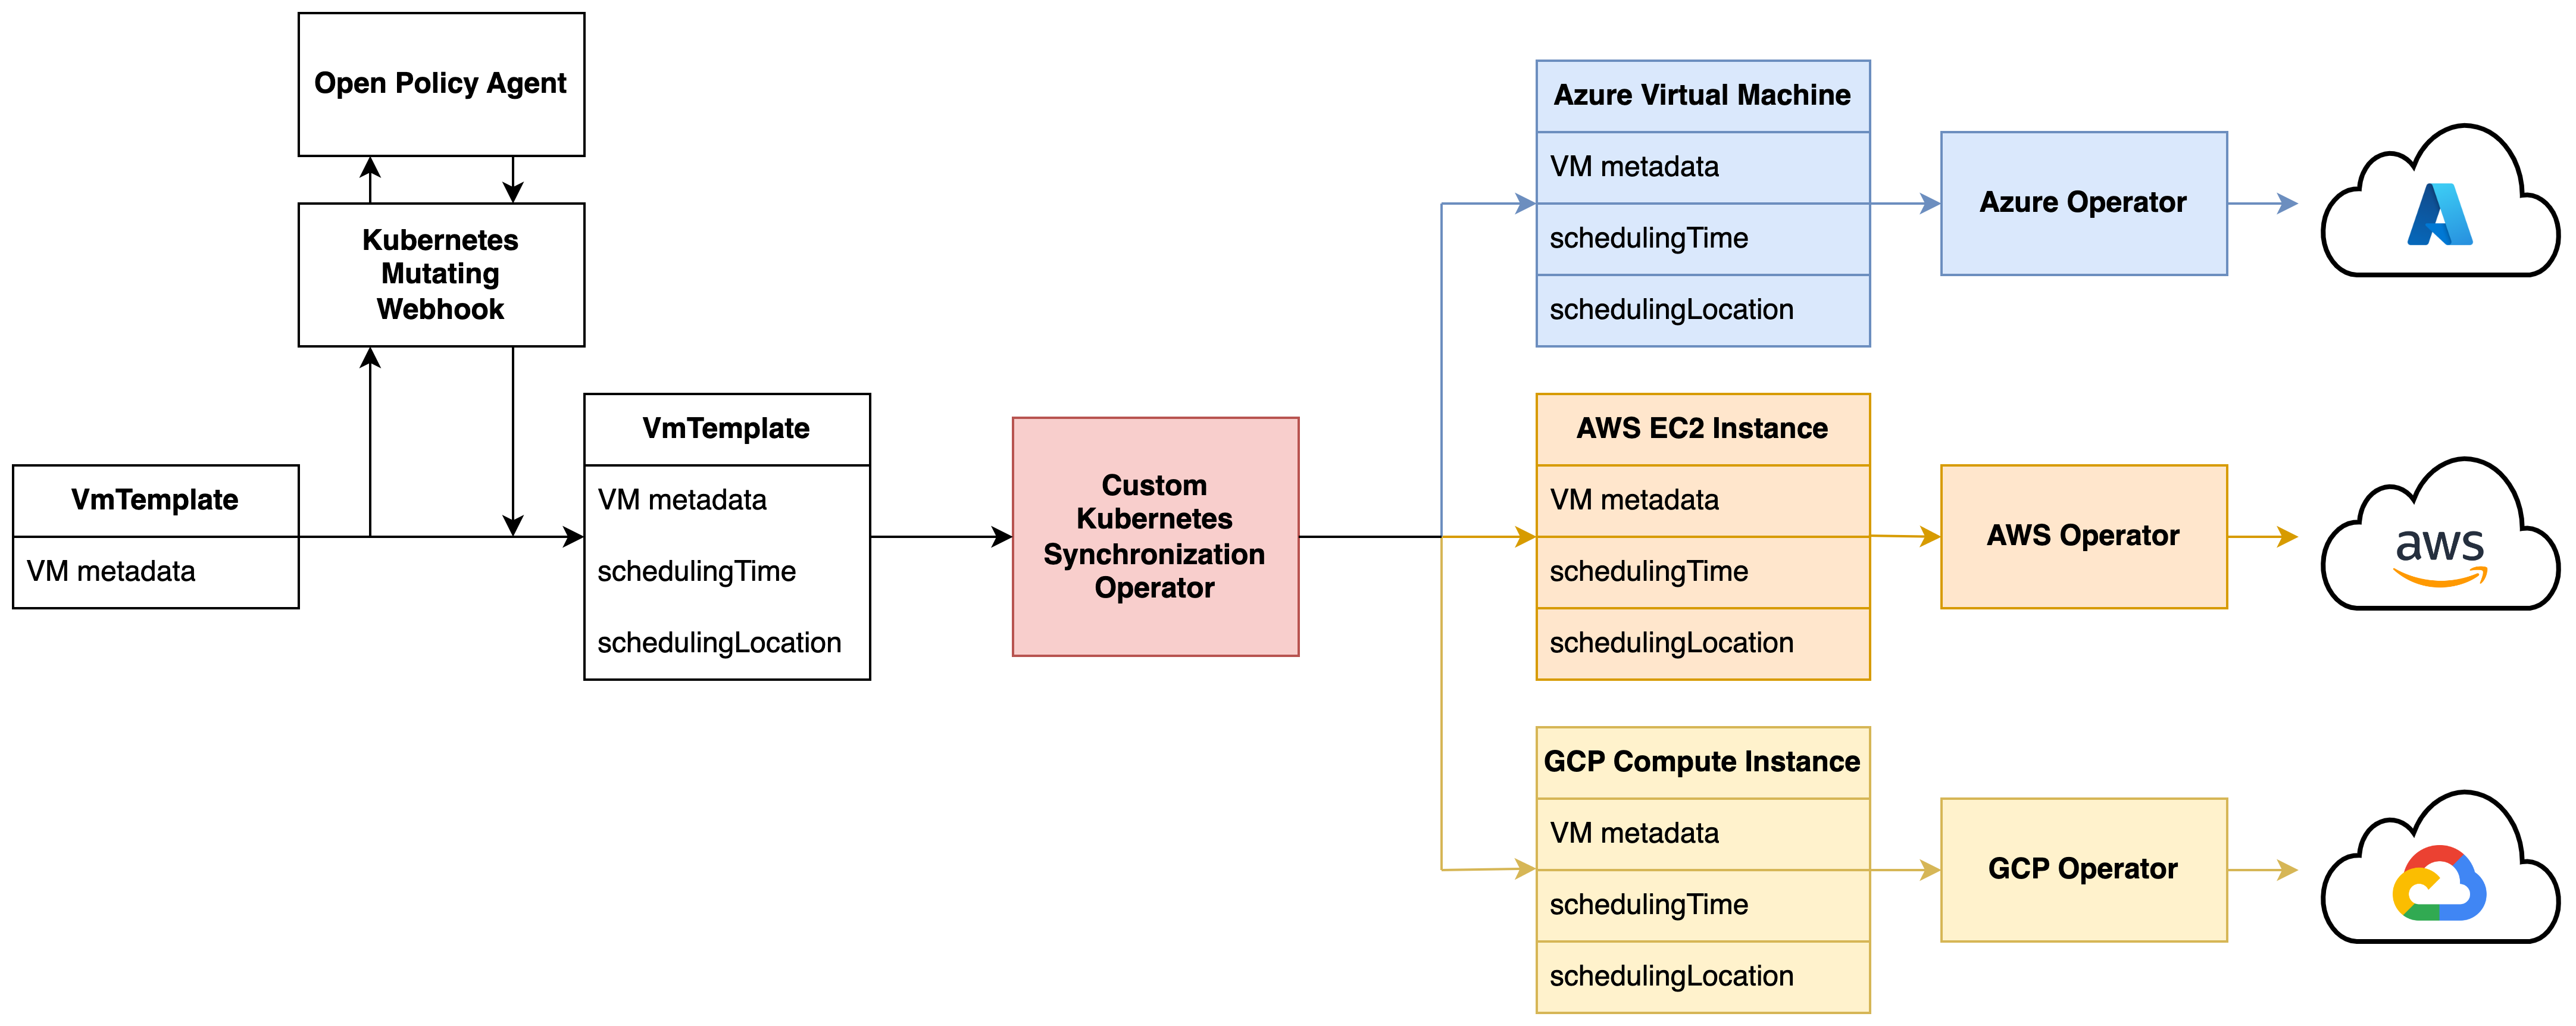
\includegraphics[width=1\linewidth]{images/k8s_operator.png}
  \caption{Multi-cloud resource management with Custom Kubernetes ``Synchronization Operator'' approach}
  \label{fig:k8s_operator}
\end{figure}

\subsection{Resource management: the Krateo PlatformOps approach}

\begin{figure}[htb]
  \centering
  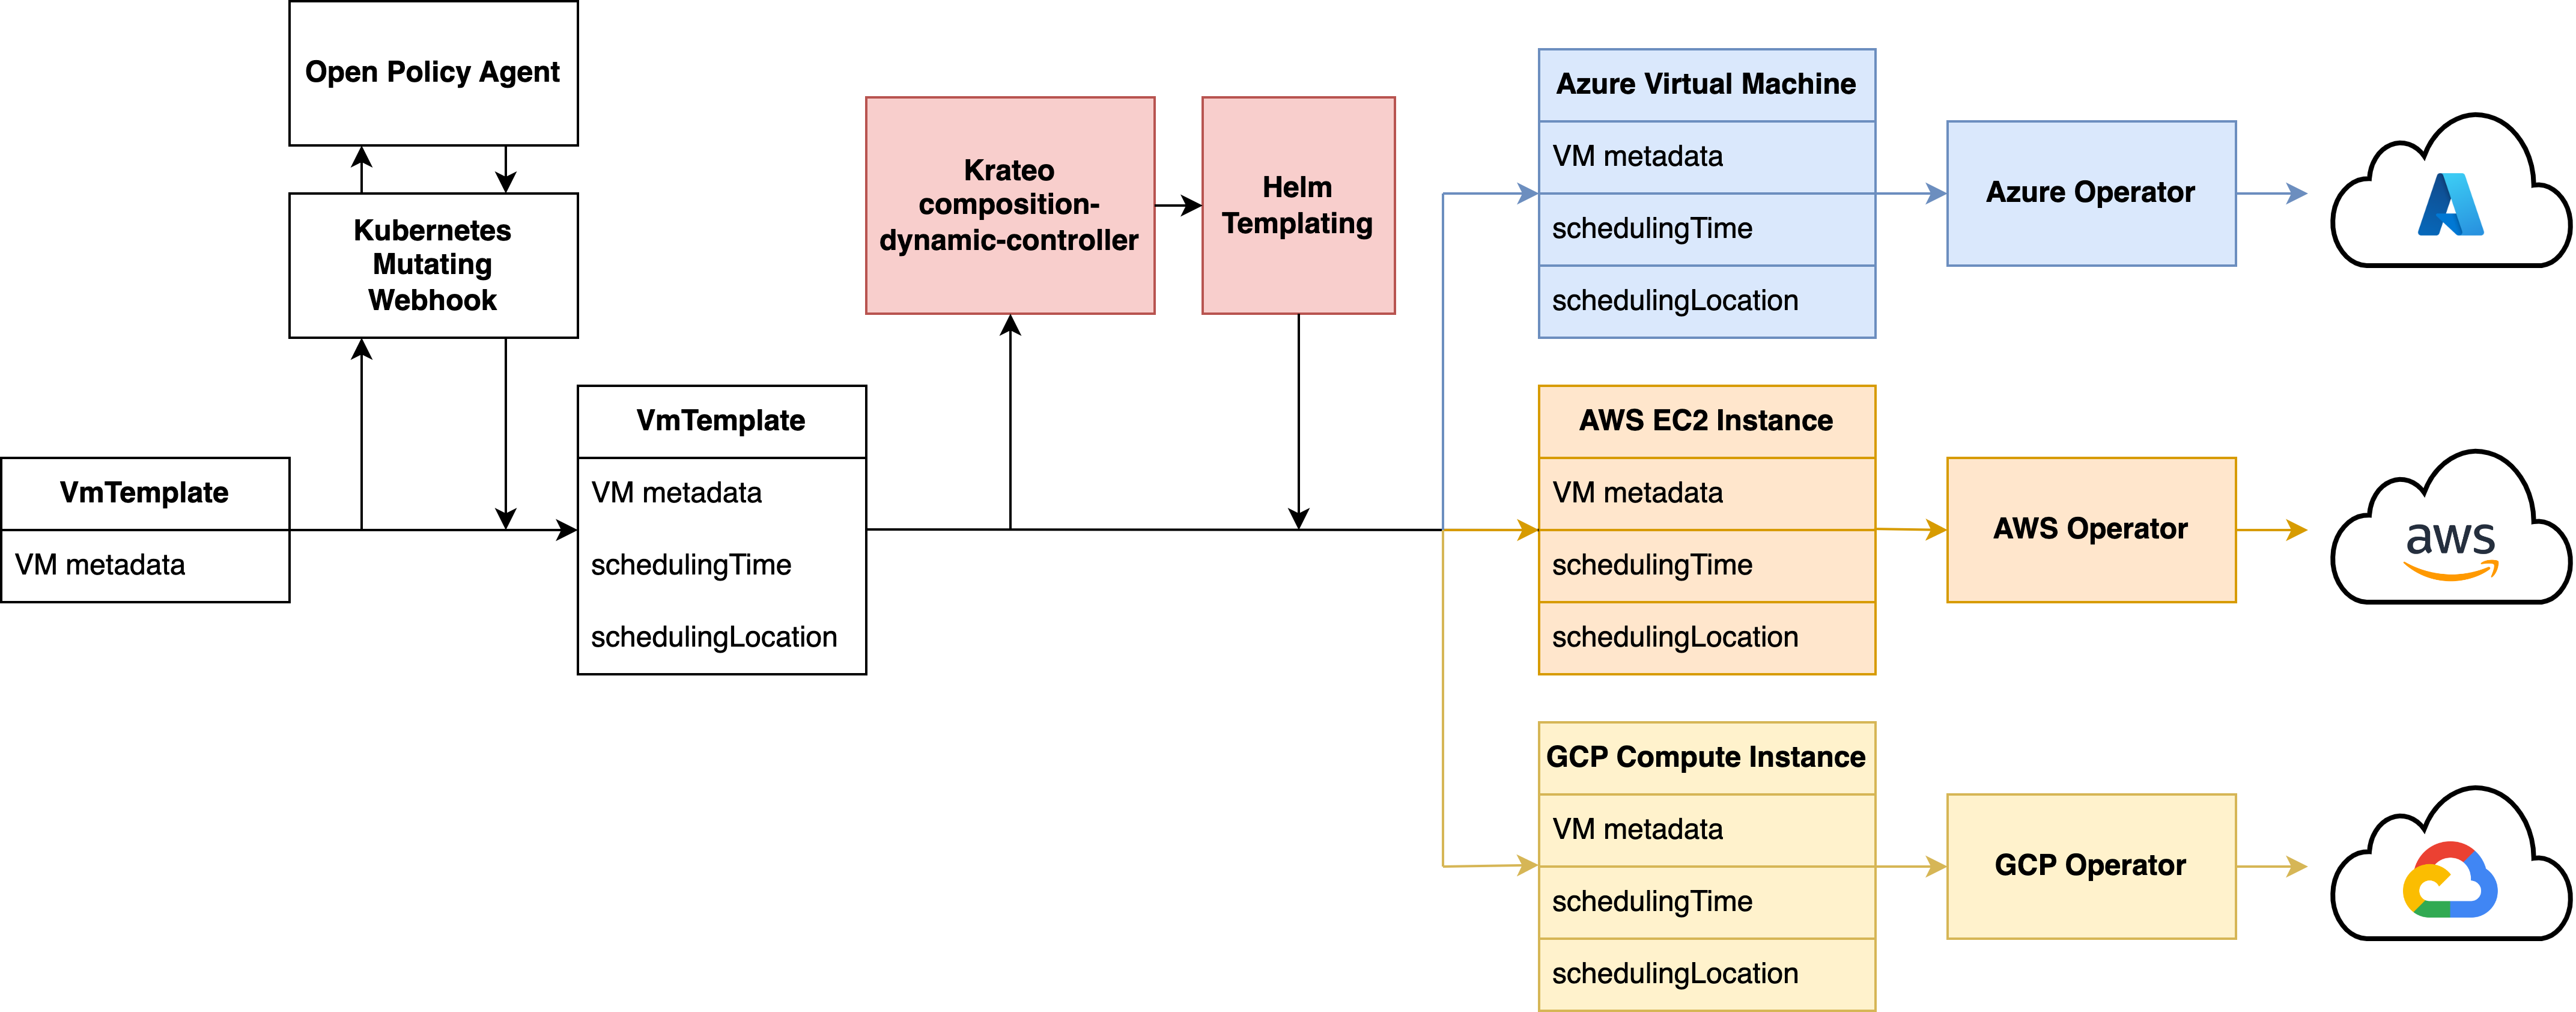
\includegraphics[width=1\linewidth]{images/krateo.png}
  \caption{Multi-cloud resource management with Krateo PlatformOps approach}
  \label{fig:krateo}
\end{figure}

In our approach, we opted to logically replace a custom Kubernetes operator (``Synchronization Operator''), originally designed to handle the \textbf{mapping} from generic to cloud-specific resources, with \textbf{Krateo Core Provider}. 
This decision was motivated by the need for \textbf{greater flexibility and maintainability} in defining multi-cloud infrastructure components. 
As a matter of fact, a custom Kubernetes operator was originally designed to handle only virtual machines (VMs).
Mappings and extensions to support additional cloud resources would have required significant code changes and maintenance overhead for each additional resource type added.
Therefore, instead of embedding business logic directly within a custom Kubernetes operator, in the current system implementation, we leverage the capabilities of \textbf{Helm templating} to dynamically generate cloud-provider-specific resources. 
More precisely, another Krateo component, the \textbf{Krateo composition-dynamic-controller} is leveraging \textbf{Helm Template Engine} under the hood to generate Kubernetes resources starting from Helm templates.
By adopting an Helm-based resource generation, we can reduce the maintenance overhead and simplify the system architecture.
Figure \ref{fig:krateo} illustrates, in a high-level manner, the revised system architecture for resource management with Krateo PlatformOps.

This approach, further described in this section, offers several advantages:
\begin{itemize}[itemsep=0.2pt, topsep=1pt]
  \item[$\bullet$] Simplified resource management: Helm enables a standardized way define resources without developing complex operator logic.
  \item[$\bullet$] Greater extensibility: By externalizing the logic from the Custom Operator (effectively removing it), future modifications and integrations on the system with additional cloud providers become easier.
  \item[$\bullet$] Reduced maintenance overhead: Custom operators typically require constant updates and refinements, especially if they are responsible for complex business logic. 
\end{itemize}

\subsubsection{Generic VM resource definition}

%n pratica, la prima fase è la creazione del composition-dynamic-controller (cdc), fatta dal core-provider
%Il core-provider non ha bisogno dei valori nella composition resource ma solo delle Custom Resource Definition, poi il cdc crea la composition facendo il templating
%Nel caso in cui si aggiornasse la composition resource con valori aggiuntivi (dal mutating webhook per esempio), sarà rifatto il templating e farà l'Helm upgrade

In order to define a generic VM resource, we leverage Krateo Core Provider to define a \textbf{CompositionDefinition} resource that specifies the structure of the VM resource.
Effectively a CompositionDefinition is a Kubernetes Custom Resource that defines the structure of a Composition Custom Resource (instance) which is an Helm chart comprised of Helm templates and values.
As a matter of fact, a CompositionDefinition is referencing a versioned Helm chart that is stored in a Helm repository (e.g. on a Helm repository server).

\begin{lstlisting}[language=yaml, caption={CompositionDefinition}, label={lst:composition_definition}]
apiVersion: core.krateo.io/v1alpha1
kind: CompositionDefinition
metadata:
  name: vmtemplate
spec:
  chart:
    repo: vm-template
    url: https://leonardovicentini.com/helm-charts/charts
    version: 1.2.0
\end{lstlisting}

The Helm chart referenced in the CompositionDefinition contains the Helm templates and values needed to define the resource named \textit{VmTemplate}.
Listing \ref{lst:values.yaml} shows an example of the VmTemplate values.yaml file, which defines the fields of the VM resource while listing \ref{lst:values.schema.json} shows the corresponding JSON schema for the values.yaml file.

\begin{lstlisting}[language=yaml_1, caption={values.yaml}, label={lst:values.yaml}, float=htpb]
# @param {string} vmName Name of the VM
vmName: test-vm

# @param {integer} cpu  Number of CPU cores
cpu: 1

# @param {integer} memory Number of GB of RAM
memory: 2

# @param {string} [schedulingTime] Scheduling Time for the VM
schedulingTime: 2025-05-05T00:00:00Z

# @param {string} [schedulingLocation] Scheduling Location for the VM
schedulingLocation: italynorth

# @param {string} duration Duration of the Workload
duration: 3h

# @param {string} deadline Deadline of the Workload
deadline: 2025-12-31T10:00:00Z

# @param {integer} maxLatency Maximum Latency of the Workload
maxLatency: 100
\end{lstlisting}

\newpage

\lstset{style=jsonstyle}
\begin{lstlisting}[caption={values.schema.json}]
{
  "type": "object",
  "$schema": "http://json-schema.org/draft-07/schema",
  "required": [
    "vmName",
    "cpu",
    "memory",
    "duration",
    "deadline",
    "maxLatency"
  ],
  "properties": {
    "vmName": {
      "type": [
        "string"
      ],
      "description": "Name of the VM",
      "default": "test-vm"
    },
    "cpu": {
      "type": [
        "integer"
      ],
      "description": "Number of CPU cores",
      "default": "1"
    },
    "memory": {
      "type": [
        "integer"
      ],
      "description": "Number of GB of RAM",
      "default": "2"
    },
    "schedulingTime": {
      "type": [
        "string"
      ],
      "description": "Scheduling Time for the VM",
      "default": "2025-05-05T00:00:00Z"
    },
    "schedulingLocation": {
      "type": [
        "string"
      ],
      "description": "Scheduling Location for the VM",
      "default": "italynorth"
    },
    "duration": {
      "type": [
        "string"
      ],
      "description": "Duration of the Workload",
      "default": "3h"
    },
    "deadline": {
      "type": [
        "string"
      ],
      "description": "Deadline of the Workload",
      "default": "2025-12-31T10:00:00Z"
    },
    "maxLatency": {
      "type": [
        "integer"
      ],
      "description": "Maximum Latency of the Workload",
      "default": "100"
    }
  }
}
  
\end{lstlisting}

\subsubsection{Generic VM to Cloud Provider Specific VM mapping}

The Krateo composition-dynamic-controller (Krateo cdc) is responsible for creating the Composition Custom Resource (instance) by templating the Helm chart referenced in the CompositionDefinition.
For the purpose of the system, we leveraged Helm templating to dynamically generate cloud-provider-specific resources from a generic VM resource.
As a matter of fact, the Helm chart contains all the \textbf{three cloud provider specific sets of templates} necessary for a VM provisioning but \textbf{only one set of templates is used at a time}.
The Krateo cdc will generate the cloud-provider-specific VM resources based on the cloud provider specified in the generic VM resource.
Therefore, for each generic VM resource, the Krateo cdc will use \textbf{only one set of templates} to generate the cloud provider specific VM resource.
This ``brokering mechanism'' (routing through Helm templates) is implemented in the Helm templates using ``\textbf{guards}'' as reported in listing \ref{lst:guards}
The manifest will be created only if the cloud provider specified in the generic VM resource is the same as the cloud provider specified in the generic VM resource.
This flexibility allows the system to be cloud-agnostic and to support multiple cloud providers as soon as the cloud provider specific templates are available in the Helm chart.
The directory structure of the Helm chart is the following:

\vspace{0.5cm}

\dirtree{%
.1 chart/.
.2 [several utilities files for mappings (omitted)].
.2 templates/.
.3 aws/.
.4 instance.yaml.
.4 subnet.yaml.
.4 vpc.yaml.
.3 azure/.
.4 networkinterface.yaml.
.4 virtualmachine.yaml.
.4 virtualnetwork.yaml.
.4 virtualnetworksubnet.yaml.
.3 gcp/.
.4 computeinstance.yaml.
.4 computenetwork.yaml.
.4 computesubnetwork.yaml.
.3 \_helpers.tpl.
.2 Chart.yaml.
.2 values.schema.json.
.2 values.yaml.
}

\vspace{0.5cm}

\begin{lstlisting}[language=yaml, caption={Helm Template guards example}, label={lst:guards}]
{{ if hasKey .Values "provider" }}
{{ $provider := .Values.provider }}
{{ if eq $provider "azure" }}
...
apiVersion: compute.azure.com/v1api20220301
kind: VirtualMachine
metadata:
  name: {{ .Values.vmName }}
...
\end{lstlisting}


\textbf{VM size selection} is a crucial step in the VM provisioning process.
Helm allows the definition of \textbf{helper functions} which resides in the \textit{\_helpers.tpl} file.
In our case, we defined a helper function called \textbf{\textit{findBestVmSize()}} that takes as input the CPU and RAM requirements of the VM and returns the best provider-specific VM size available.
For instance: a generic requested VM specification could be (4 vCPU, 8 GiB of RAM) and this would be mapped to the ``\textit{Azure Standard\_A4\_v2}'' VM size.
A prerequisite for that is to have a mapping between the tuple (CPU, RAM) and the VM sizes (a string) for each cloud provider.
This mappings are built using the cloud provider documentation and are stored in the Helm chart as a set of utilities files.
Potentially, an automatic way to fetch the available VM sizes for each cloud provider could be implemented in the future.
For our first iteration of the system we used a small subset of all the available instance types (i.e. 5 instance types for each cloud provider).

\subsubsection{Scheduling time waiting logic}
\label{sec:scheduling_time_waiting_logic}

Helm template engine is also leveraged to handle the \textbf{scheduling time waiting logic}.
As previously described in section \ref{sec:limitations_custom_operator}, this logic is crucial for the system due to the fact that cloud provider operators do not support scheduling time metadata in their CRs and therefore as soon as a CR is created the cloud provider operator will provision the resource immediately.
It must be remembered that is not a trivial task to implement this logic in a Kubernetes operator.
In this case, we leverage a set of ``\textbf{guards}'' to effectively block manifest creation until the scheduling time is reached. 
As a result, only when the scheduling time is reached the manifest is created and applied by Helm and finally the resource is provisioned by the cloud provider operator.
As a matter of fact, Krateo cdc will periodically perform an ``helm upgrade'' and if the scheduling time is reached the cloud provider specific resources will be created. 
As a consequence, the specific cloud provider operator will be triggered by the creation of the cloud provider specific resources and will provision the VM.
Listing \ref{lst:sched} shows an example of how guards are used to handle the scheduling time waiting logic and other scheduling constraints.
We also make sure, for instance, that the generic CR contains a ``provider'' field that specifies the cloud provider where the resource should be provisioned.

\begin{lstlisting}[language=yaml, caption={Scheduling time}, label={lst:sched}]
{{ if hasKey .Values "provider" }}
{{ $provider := .Values.provider }}
{{ if eq $provider "azure" }}

{{ if hasKey .Values "schedulingTime" }}
{{ $schedulingTime := .Values.schedulingTime | toDate "2006-01-02T15:04:05Z" }}
{{ $now := now }}
@\yellowhl{\{\{{ if \$now.After \$schedulingTime \}\}} }@
{{ if $now.After $schedulingTime }}
...
apiVersion: compute.azure.com/v1api20220301
kind: VirtualMachine
metadata:
  name: {{ .Values.vmName }}
...
\end{lstlisting}

In order to take into account the time needed for the cloud provider operator to provision the resource, additional logic could be added in the template to anticipate the scheduling time (e.g, using a \textit{provisioningTimeOffset}).

\section{Multi-Cloud Integration through Kubernetes Operators}
\label{sec:cloud_providers_operators}

The integration of operators from different cloud providers has enabled the development of an effective \textbf{multi-cloud system}, allowing seamless orchestration and provisioning of cloud resources across various cloud platforms. 
More precisely, the system leverages Kubernetes operators from \textbf{Microsoft Azure}, \textbf{Google Cloud Platform (GCP)}, and \textbf{Amazon Web Services (AWS)}.
Each Operator, when installed on a Kubernetes cluster, installs a \textbf{set of Custom Resource Definitions (CRDs)} that represent cloud resources specific to the cloud provider.
These CRDs can be used to define cloud resources in a declarative manner, in the form of Kubernetes Custom Resources (CRs), allowing users to specify the desired state of the cloud resources they wish to manage.
The other component installed by the Operator is the \textbf{controller}, a software module that watches for changes to the Custom Resources in the cluster and takes all the necessary actions to reconcile the actual state with the desired state.
Under the hood the controller interacts with the cloud provider's API to provision, update, and delete cloud resources.
Kubernetes operators work on the principle of \textbf{Continuous Reconciliation}, ensuring, in this case, that the desired state of the system, as defined by users, aligns with the actual state of provisioned cloud resources. 
In particular, Operators act as controllers that monitor (\textit{watch}), adjust, and manage external cloud resources within a Kubernetes environment. 
Inside the Kubernetes cluster lie the \textbf{real-time representation of the provisioned cloud resources}, which are managed by the operators.
It must be noted that different cloud providers adopt \textbf{different design choices} for their Kubernetes operators and more in general for their overall cloud infrastructure management. 
Therefore, for the creation of logically similar resources, like a virtual machine, the structure and the field of the resources can be different. 
These resources typically include:
\begin{itemize}[itemsep=0.2pt, topsep=1pt]
  \item[$\bullet$] Compute resources (e.g., VM instances, virtual machine templates)
  \item[$\bullet$] Networking components (e.g., virtual networks, subnets, security groups)
  \item[$\bullet$] Storage allocations (e.g., persistent volumes, cloud disks)
  \item[$\bullet$] Access management (e.g., resource groups, roles, authentication credentials)
\end{itemize}

For the purpose of this work we defined a \textbf{baseline infrastructure} for each cloud provider taken into account in order to have a common ground for the system to work. 
This baseline infrastructure is composed by the minimum set of resources needed for a VM provisioning.
Each public cloud provider has its complexities and nuances when it comes to managing cloud resources.
In the following sections, we provide an overview of the minimum set of resources needed for VM provisioning on each cloud provider, as well as some of the specific configurations required for each resource.
We deem useful to provide a table summarizing some of the key fields that are needed for VM provisioning.
This fields are labeled with an ID which will be attached to the resources' listings in the following sections.

\begin{table}[H]
  \centering
  \begin{tabular}{|l|l|}
  \hline
  \textbf{ID} & \textbf{VM field} \\ \hline
  1           & Scheduling region \\ \hline
  2           & VM size           \\ \hline
  3           & Operating System           \\ \hline
  \end{tabular}
  \caption{Key fields for VM provisioning}
  \label{tab:vm_fields}
\end{table}

\subsection{Azure Kubernetes Operator}

Microsoft Azure provides a Kubernetes operator called \textbf{Azure Service Operator v2} (ASO).
Currently, ASO supports more than 150 different Azure resources one of which is the \textbf{Azure Virtual Machine}.
An example of a Azure Virtual Machine custom resource is the one illustrated in listing \ref{lst:azure}.
The minimum set of resources needed for VM provisioning on Azure through Azure service operator is:

\begin{itemize}[itemsep=0.2pt, topsep=1pt] 
\item[$\bullet$] Virtual Network 
\item[$\bullet$] Virtual Network Subnet
\item[$\bullet$] Network Interface
\item[$\bullet$] Virtual Machine
\end{itemize}

\begin{figure}[H]
\centering
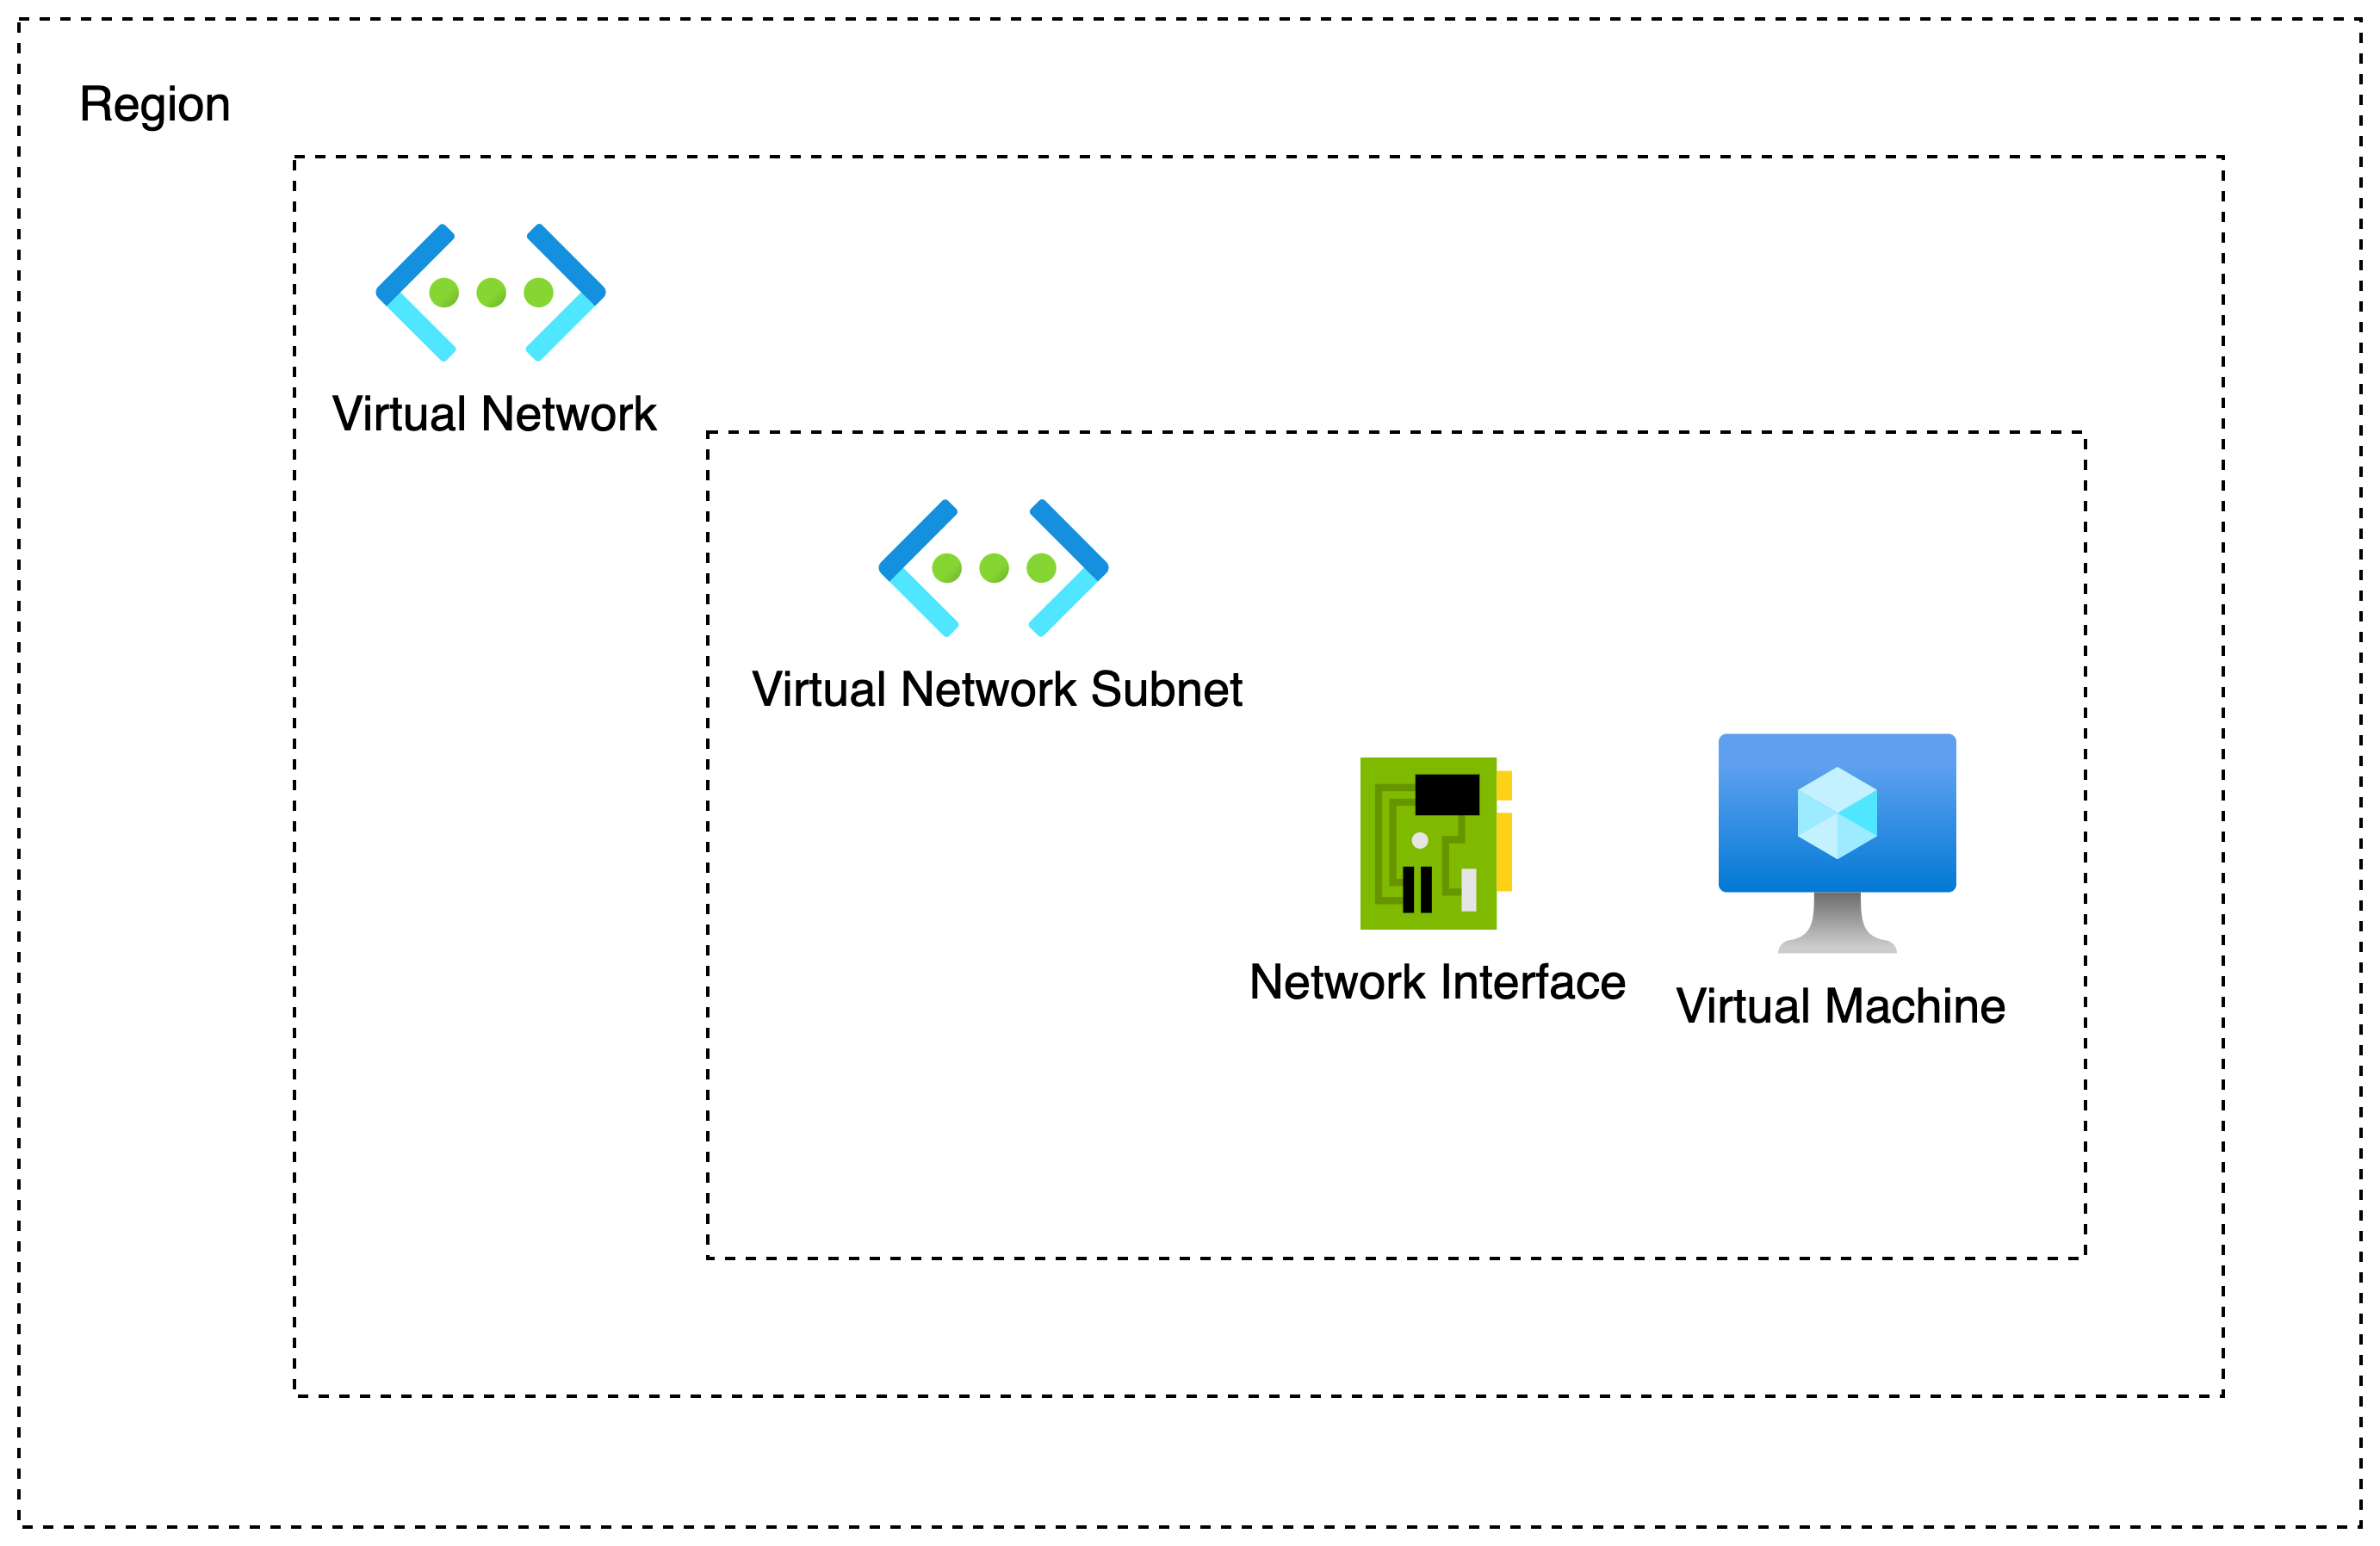
\includegraphics[width=0.75\linewidth]{images/azure.png}
\caption{Minimum set of Azure resources for VM provisioning}
\label{fig:azure}
\end{figure}

\begin{lstlisting}[language=yaml, caption={Azure Instance Custom Resource}, label={lst:azure}]
apiVersion: compute.azure.com/v1api20220301
kind: VirtualMachine
metadata:
  name: {{ .Values.vmName }}
  namespace: {{ .Values.namespace | default "greenops" }}
spec:
  hardwareProfile:
   @\yellowhl{    vmSize: \{\{{ \$vmSize \}\}} \#[2] }@
   @\yellowhl{    location: \{\{{ .Values.schedulingLocation \}\}} \#[1] }@
  networkProfile:
    networkInterfaces:
    - reference:
        group: network.azure.com
        kind: NetworkInterface
        name: {{ .Values.vmName }}-{{ $av.networkInterface.suffix }}
  osProfile: {{ $av.virtualMachine.osProfile | toYaml | nindent 4 }}
  owner:
    armId: {{ $av.resourceGroup.armId }}
  storageProfile:
   @\yellowhl{    imageReference: \#[3] }@
      publisher: Canonical
      offer: 0001-com-ubuntu-server-jammy
      sku: 22_04-lts
      version: latest
\end{lstlisting}

\subsection{GCP Operator}

Google Cloud Platform provides a Kubernetes operator called \textbf{GCP Config Connector}.
The name of the virtual machine resource in GCP is \textbf{ComputeInstance}.
An example of a GCP ComputeInstance custom resource is the one illustrated in listing \ref{lst:gcp}.
For what concerns the GCP Operator, the minimum set of resources needed for VM provisioning is:

\begin{itemize}[itemsep=0.2pt, topsep=1pt] 
  \item[$\bullet$] Compute Network
  \item[$\bullet$] Compute SubNetwork
  \item[$\bullet$] Compute Instance
  \end{itemize}

\begin{figure}[H]
\centering
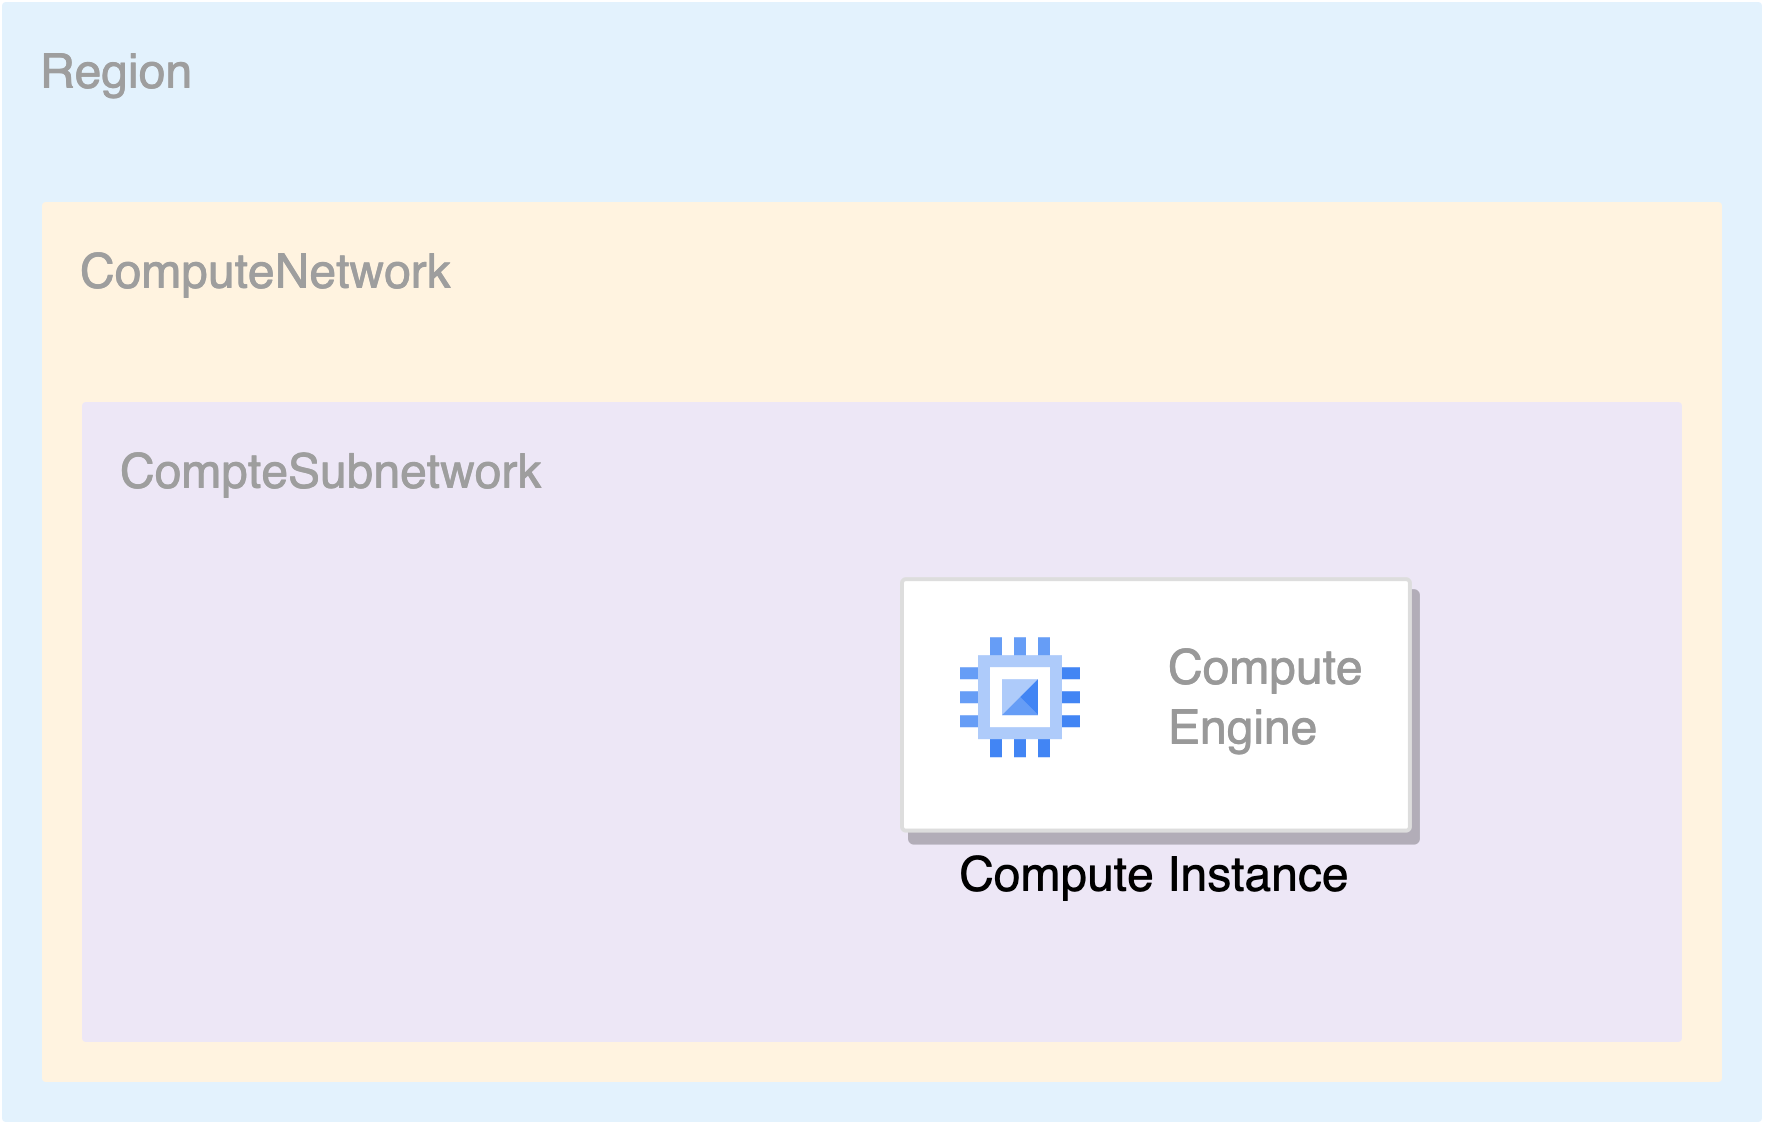
\includegraphics[width=0.75\linewidth]{images/gcp.png}
\caption{Minimum set of GCP resources for VM provisioning}
\label{fig:gcp}
\end{figure}

We can mention the fact that some fields on GCP resource manifests are based on regions and some fields are based on avavilability zones.
In order to select a zone, a helper function is used to select a zone based on the region.

\begin{lstlisting}[language=yaml, caption={GCP Intance Custom Resource}, label={lst:gcp}]
  apiVersion: compute.cnrm.cloud.google.com/v1beta1
  kind: ComputeInstance
  metadata:
    name: {{ .Values.vmName }}
    namespace: {{ .Values.namespace | default "greenops" }}
  spec:
   @\yellowhl{    machineType: \{\{{ \$vmSize \}\}} \#[2] }@
    machineType: {{ $vmSize }} [2]
   @\yellowhl{    zone: \{\{{ \$zone \}\}} \#[1] }@
    zone: {{ $zone }} [1]
    bootDisk:
      initializeParams:
        size: 24
        type: pd-ssd
        sourceImageRef:
         @\yellowhl{    external: debian-cloud/debian-11 \#[3] }@
          external: debian-cloud/debian-11
    networkInterface:
      - subnetworkRef:
          name: {{ .Values.vmName }}-subnetwork
        aliasIpRange:
          - ipCidrRange: /24
            subnetworkRangeName: cloudrange
\end{lstlisting}

\subsection{AWS Operator}

AWS provides an entire collection of operators that are part of the AWS controllers for Kubernetes (ACK) project.
Each controller is responsible for managing a specific AWS service, such as EC2, EBS, RDS, S3, and more. In the context of this research, the EC2 controller is used to manage virtual machines (called EC2 Instances) provisioning on AWS.
An example of a AWS EC2 Instance Custom Resource is the one illustrated in listing \ref{lst:aws}.
The minimum set of resources needed for VM provisioning is:
\begin{itemize}[itemsep=0.2pt, topsep=1pt] 
\item[$\bullet$] VPC
\item[$\bullet$] Subnet
\item[$\bullet$] Instance
\end{itemize}

\begin{figure}[H]
\centering
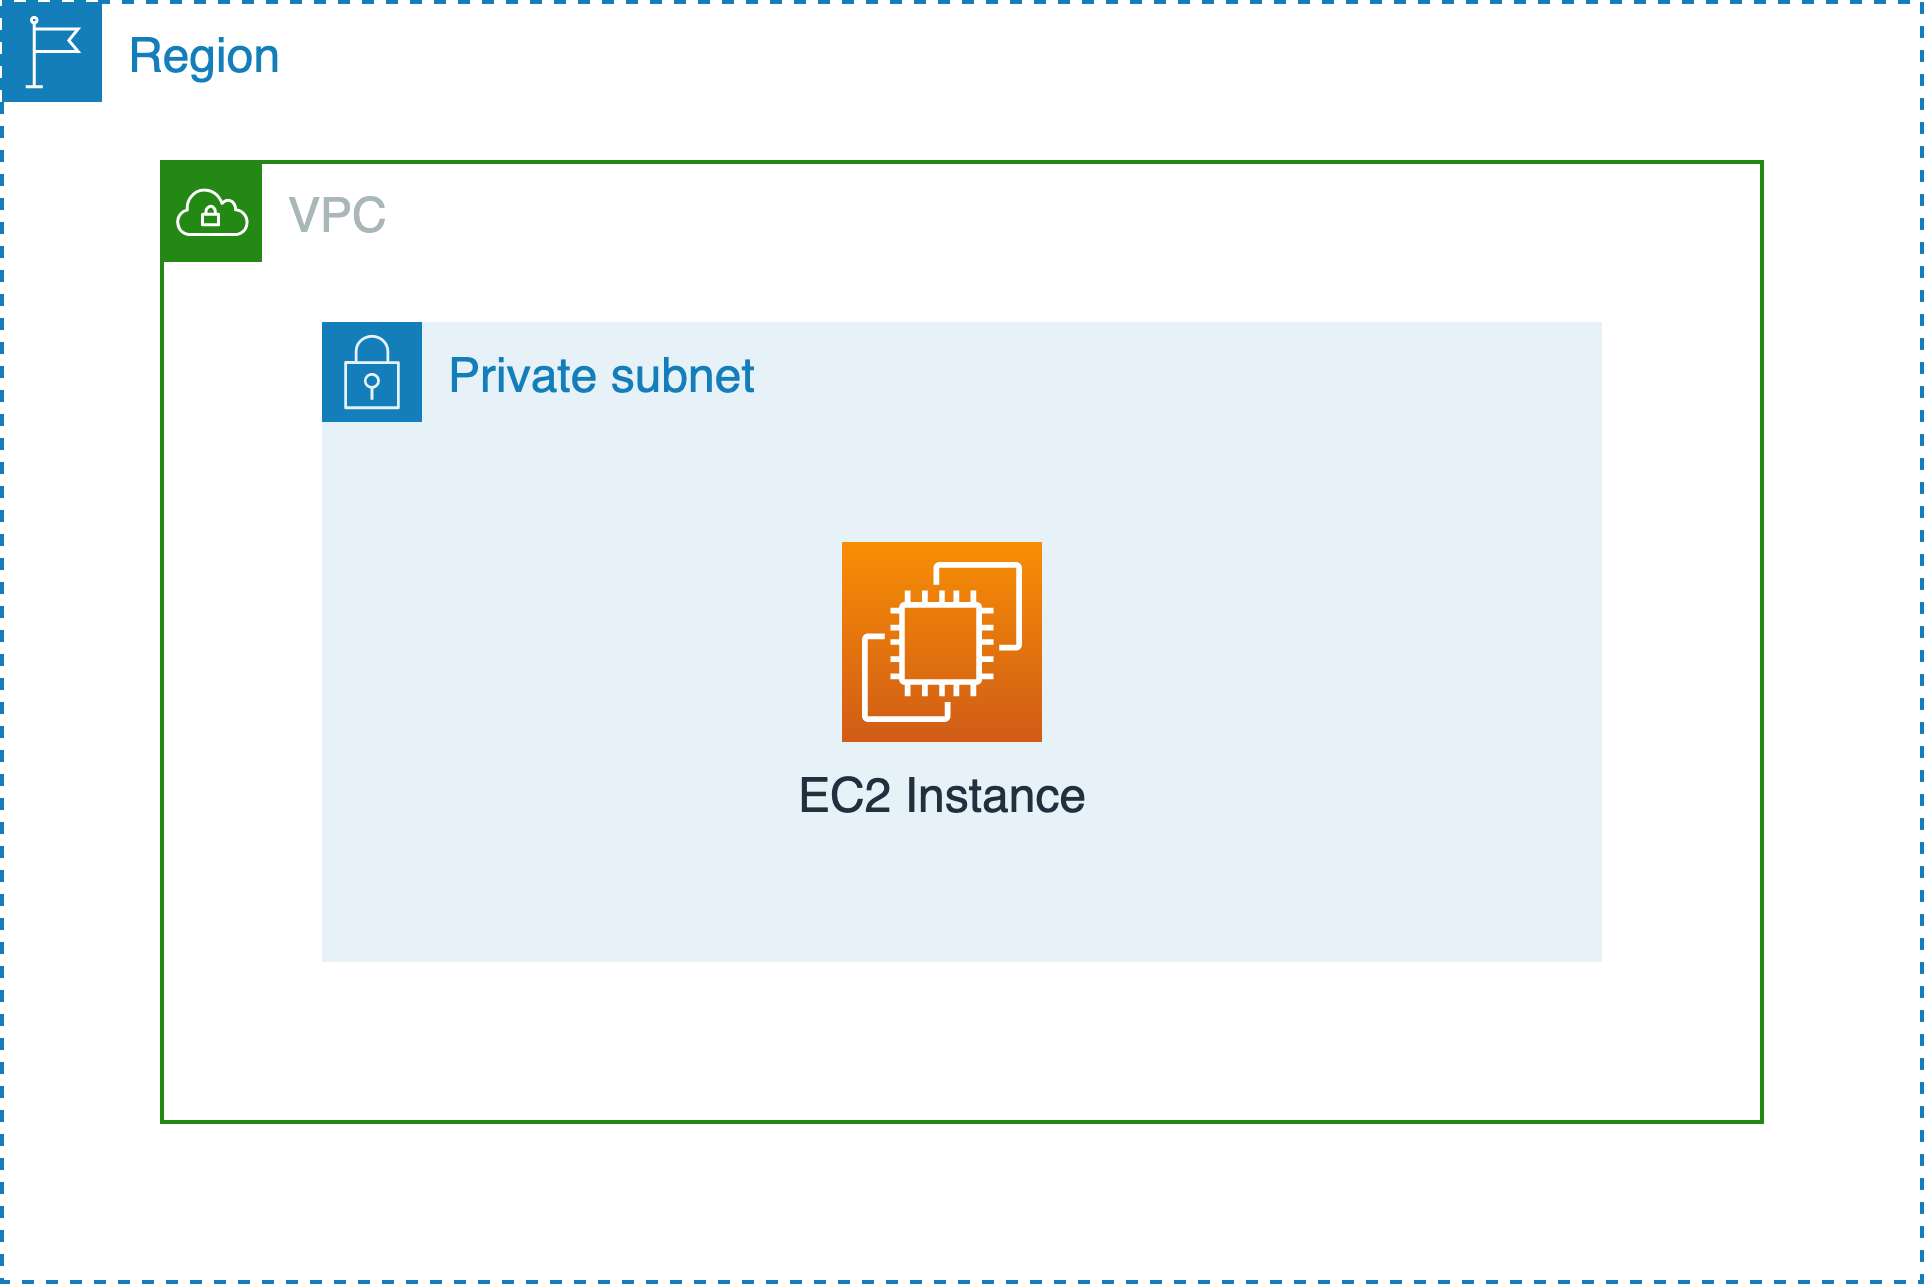
\includegraphics[width=0.75\linewidth]{images/aws.png}
\caption{Minimum set of AWS resources for VM provisioning}
\label{fig:aws}
\end{figure}

\subsubsection{Provider specific configurations}

As described at the beginning of this section, the implementation approach adopted in our system ensures compatibility with diverse cloud provider design choices. Cloud providers may impose different constraints and best practices when managing Kubernetes-native resources, and the system is designed to adapt to these variations seamlessly.
One notable design choice observed with the AWS operator is the restriction on referencing some Kubernetes objects inside a Custom Resource (CR) manifest. This limitation means that developers cannot directly link a resource (e.g., a Virtual Machine) to another Kubernetes object (e.g., a Subnet) using built-in object references.
To overcome this limitation, our system leverages \textbf{Helm’s \textit{lookup function}}, which dynamically retrieves Kubernetes object details at runtime. This method allows us to fetch required parameters without directly referencing Kubernetes objects in the CR, ensuring compatibility with the AWS operator’s design constraints. The following example demonstrates how the lookup function can be used to resolve subnet IDs dynamically and inject them into the CR manifest. \newline

\begin{lstlisting}[language=yaml, caption={Helm Lookup example: dynamically resolving SubnetIDs}, label={lst:helm_lookup}, float=htpb]
...
apiVersion: ec2.services.k8s.aws/v1alpha1
kind: Instance
metadata:
  name: {{ .Values.vmName }}
  namespace: {{ .Values.namespace | default "greenops" }}
...
spec:
  ...
  subnetID: {{ (lookup "ec2.services.k8s.aws/v1alpha1" "Subnet" (.Values.namespace | default "greenops") (printf "%s-subnet" .Values.vmName)).status.subnetID }}
...
\end{lstlisting}

The Helm lookup function can be used to look up resources in a running cluster and its synopsis is: ``lookup apiVersion, kind, namespace, name -> resource or resource list'' \cite{helm_lookup}.
In the listing \ref{lst:helm_lookup}, the Helm lookup function retrieves the subnetID from a Subnet Custom Resource dynamically, based on the VM name and namespace. Then, the subnetID is injected into the Instance Custom Resource manifest, ensuring that the VM is provisioned in the correct subnet.
An example by the same AWS Operator where instead a direct reference to a resource is allowed is the one illustrated in listing \ref{lst:aws_direct_reference}. \\

\begin{lstlisting}[language=yaml, caption={AWS Operator direct reference example}, label={lst:aws_direct_reference}]
...
apiVersion: ec2.services.k8s.aws/v1alpha1
kind: Subnet
metadata:
  name: {{ .Values.vmName }}-subnet
...
spec:
  vpcRef: 
    from: 
      name: {{ .Values.vmName }}-vpc
      namespace: {{ .Values.namespace | default "greenops" }}
...
\end{lstlisting}

In the case of Listing \ref{lst:aws_direct_reference}, the Subnet Custom Resource manifest directly references in a convenient way the VPC Custom Resource using its name and namespace since the Operator is designed to support this type of relationship. As explained before, this is determined by Operator design choices but our system is able to handle both scenarios.
\newline
Another important aspect to consider is that, when launching an Amazon EC2 instance, specifying an AMI is \textbf{mandatory}. 
An Amazon Machine Image (AMI) is a pre-configured image that provides the necessary software environment to set up and boot an Amazon EC2 instance \cite{aws_AMIs}. 
In other words, AMIs serve as a blueprint for launching virtual machines (VMs) in AWS.
The AMI must be compatible with the chosen EC2 instance type, ensuring that the selected image supports the required hardware and software configurations.
The following attributes define an AMI:
\begin{itemize}[itemsep=0.2pt, topsep=1pt] 
  \item[$\bullet$] Region: AMIs are region-specific
  \item[$\bullet$] Operating System: Determines the base OS (e.g., Ubuntu, RHEL) installed on the AMI.
  \item[$\bullet$] Processor Architecture: e.g., x86, ARM
  \item[$\bullet$] Root Device Type: Specifies whether the AMI uses an EBS-backed volume (Elastic Block Store) or Instance Store for storage.
  \item[$\bullet$] Virtualization Type: Defines whether the AMI supports paravirtual (PV) or hardware virtual machine (HVM) instances.
\end{itemize}

The most important attribute for our system is the \textbf{Operating System} since it determines the software environment for the VM.
For the purpose of this research, only \textbf{Ubuntu-based AMIs} have been considered for provisioning virtual machines. Official Ubuntu AMIs were collected from a dedicated Ubuntu repository.
In order to select the most suitable AMI for a given VM, the system leverages a custom helper function to dynamically select the appropriate AMI ID based on the region and other parameters specified in the VmTemplate Kubernetes Custom Resource (CR).

\begin{lstlisting}[language=yaml, caption={AWS}, label={lst:aws}]
apiVersion: ec2.services.k8s.aws/v1alpha1
kind: Instance
metadata:
  name: {{ .Values.vmName }}
  namespace: {{ .Values.namespace | default "greenops" }}
  annotations:
   @\yellowhl{    services.k8s.aws/region: \{\{{ .Values.schedulingLocation \}\}} \#[1] }@
spec:
 @\yellowhl{    imageID: \{\{{ \$imageID\}\}} \#[3] }@
 @\yellowhl{    instanceType: \{\{{ \$vmSize \}\}} \#[2] }@
  subnetID: {{ (lookup "ec2.services.k8s.aws/v1alpha1" "Subnet" (.Values.namespace | default "greenops") (printf "%s-subnet" .Values.vmName)).status.subnetID }}
\end{lstlisting}

\section{Kubernetes Mutating Webhook Configuration}

In the context of \textbf{Kubernetes Admission Control}, in addition to standard, compiled-in admission plugins, Kubernetes supports the use of additional admission plugins that are effectively extensions of the system and run as \textbf{webhooks} configured at runtime \cite{kubernetes_dynamic_admission_control}. 
This means that the admission control logic can be extended dynamically without the need to recompile the Kubernetes API server or other Kubernetes components. 
Changes are applied at runtime to the running Kubernetes cluster, making the system more flexible and adaptable.
Said plugins can be used to enforce custom policies and perform additional validation and mutation of Kubernetes objects before they are persisted in the cluster.
We can classify webooks in two categories: validating and mutating webhooks.
Validating webhooks are used to validate the object and reject it if it does not meet the validation criteria.
Mutating webhooks are used to modify the object before it is persisted in the cluster.
We must highlight the difference of two entities: the webhook configuration and the actual webhook server which performs mutation or validation.
The latter could be a custom server to apply custum mutation or validation logic or it could be a service ready to use out of the box like an Open Policy Agent server.

Figure \ref{fig:k8s_admission_control} shows the Kubernetes Admission Control flow with the addition of mutating and validating webhooks.
The flow can be summarized as follows:
\begin{enumerate}[itemsep=0.2pt, topsep=1pt]
  \item The K8s API server receives an API request.
  \item Authentication and authorization phase take place.
  \item Mutating webhooks are called first. If any of them returns an error, the request is rejected.
  \item The Object Schema Validation phase is executed.
  \item Validating webhooks are called. If any of them returns an error, the request is rejected.
  \item The object is persisted in the cluster.
\end{enumerate}

\begin{figure}[htb]
  \centering
  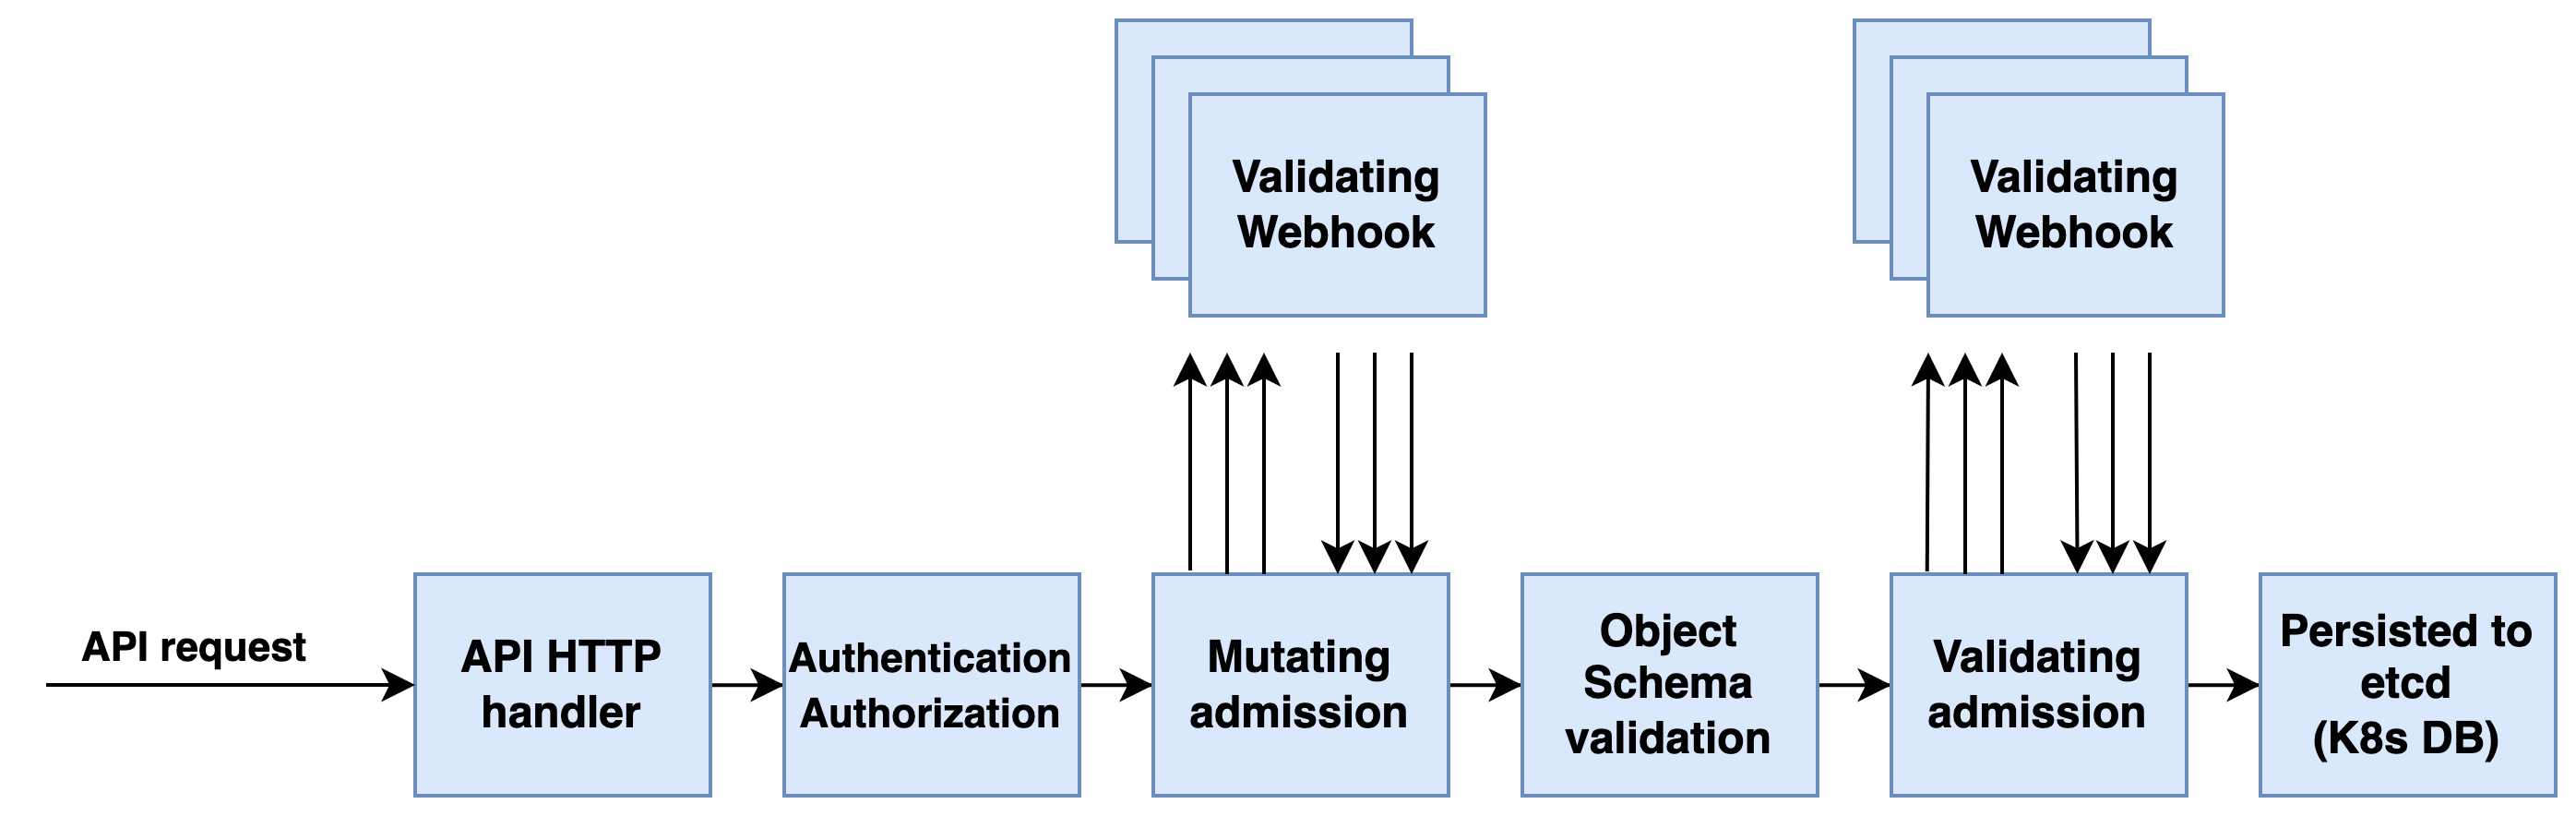
\includegraphics[width=1\linewidth]{images/k8s_admission.png}
  \caption{Kubernetes Admission Control}
  \label{fig:k8s_admission_control}
\end{figure}

A webhook service can be either a deployment with the related service inside the cluster like seen in the image \ref{fig:k8s_webhook_example} or can be a service deployed outside the cluster as long as it is reachable by the K8s API server.

Figure \ref{fig:k8s_webhook_example} shows an example of a Kubernetes Mutating Webhook. 
The webhook server is deployed as a Kubernetes Deployment (with 1 Pod), with a corresponding Service to expose it within the cluster. 
The webhook server is responsible for receiving The AdmissionReview Request, applying custom logic, and returning an AdmissionReview Response to the Kubernetes API server describing the mutation to be applied to the resource.
The custom logic in this simple example is to add a label "mutated: true" to the resource.

\begin{figure}[H]
  \centering
  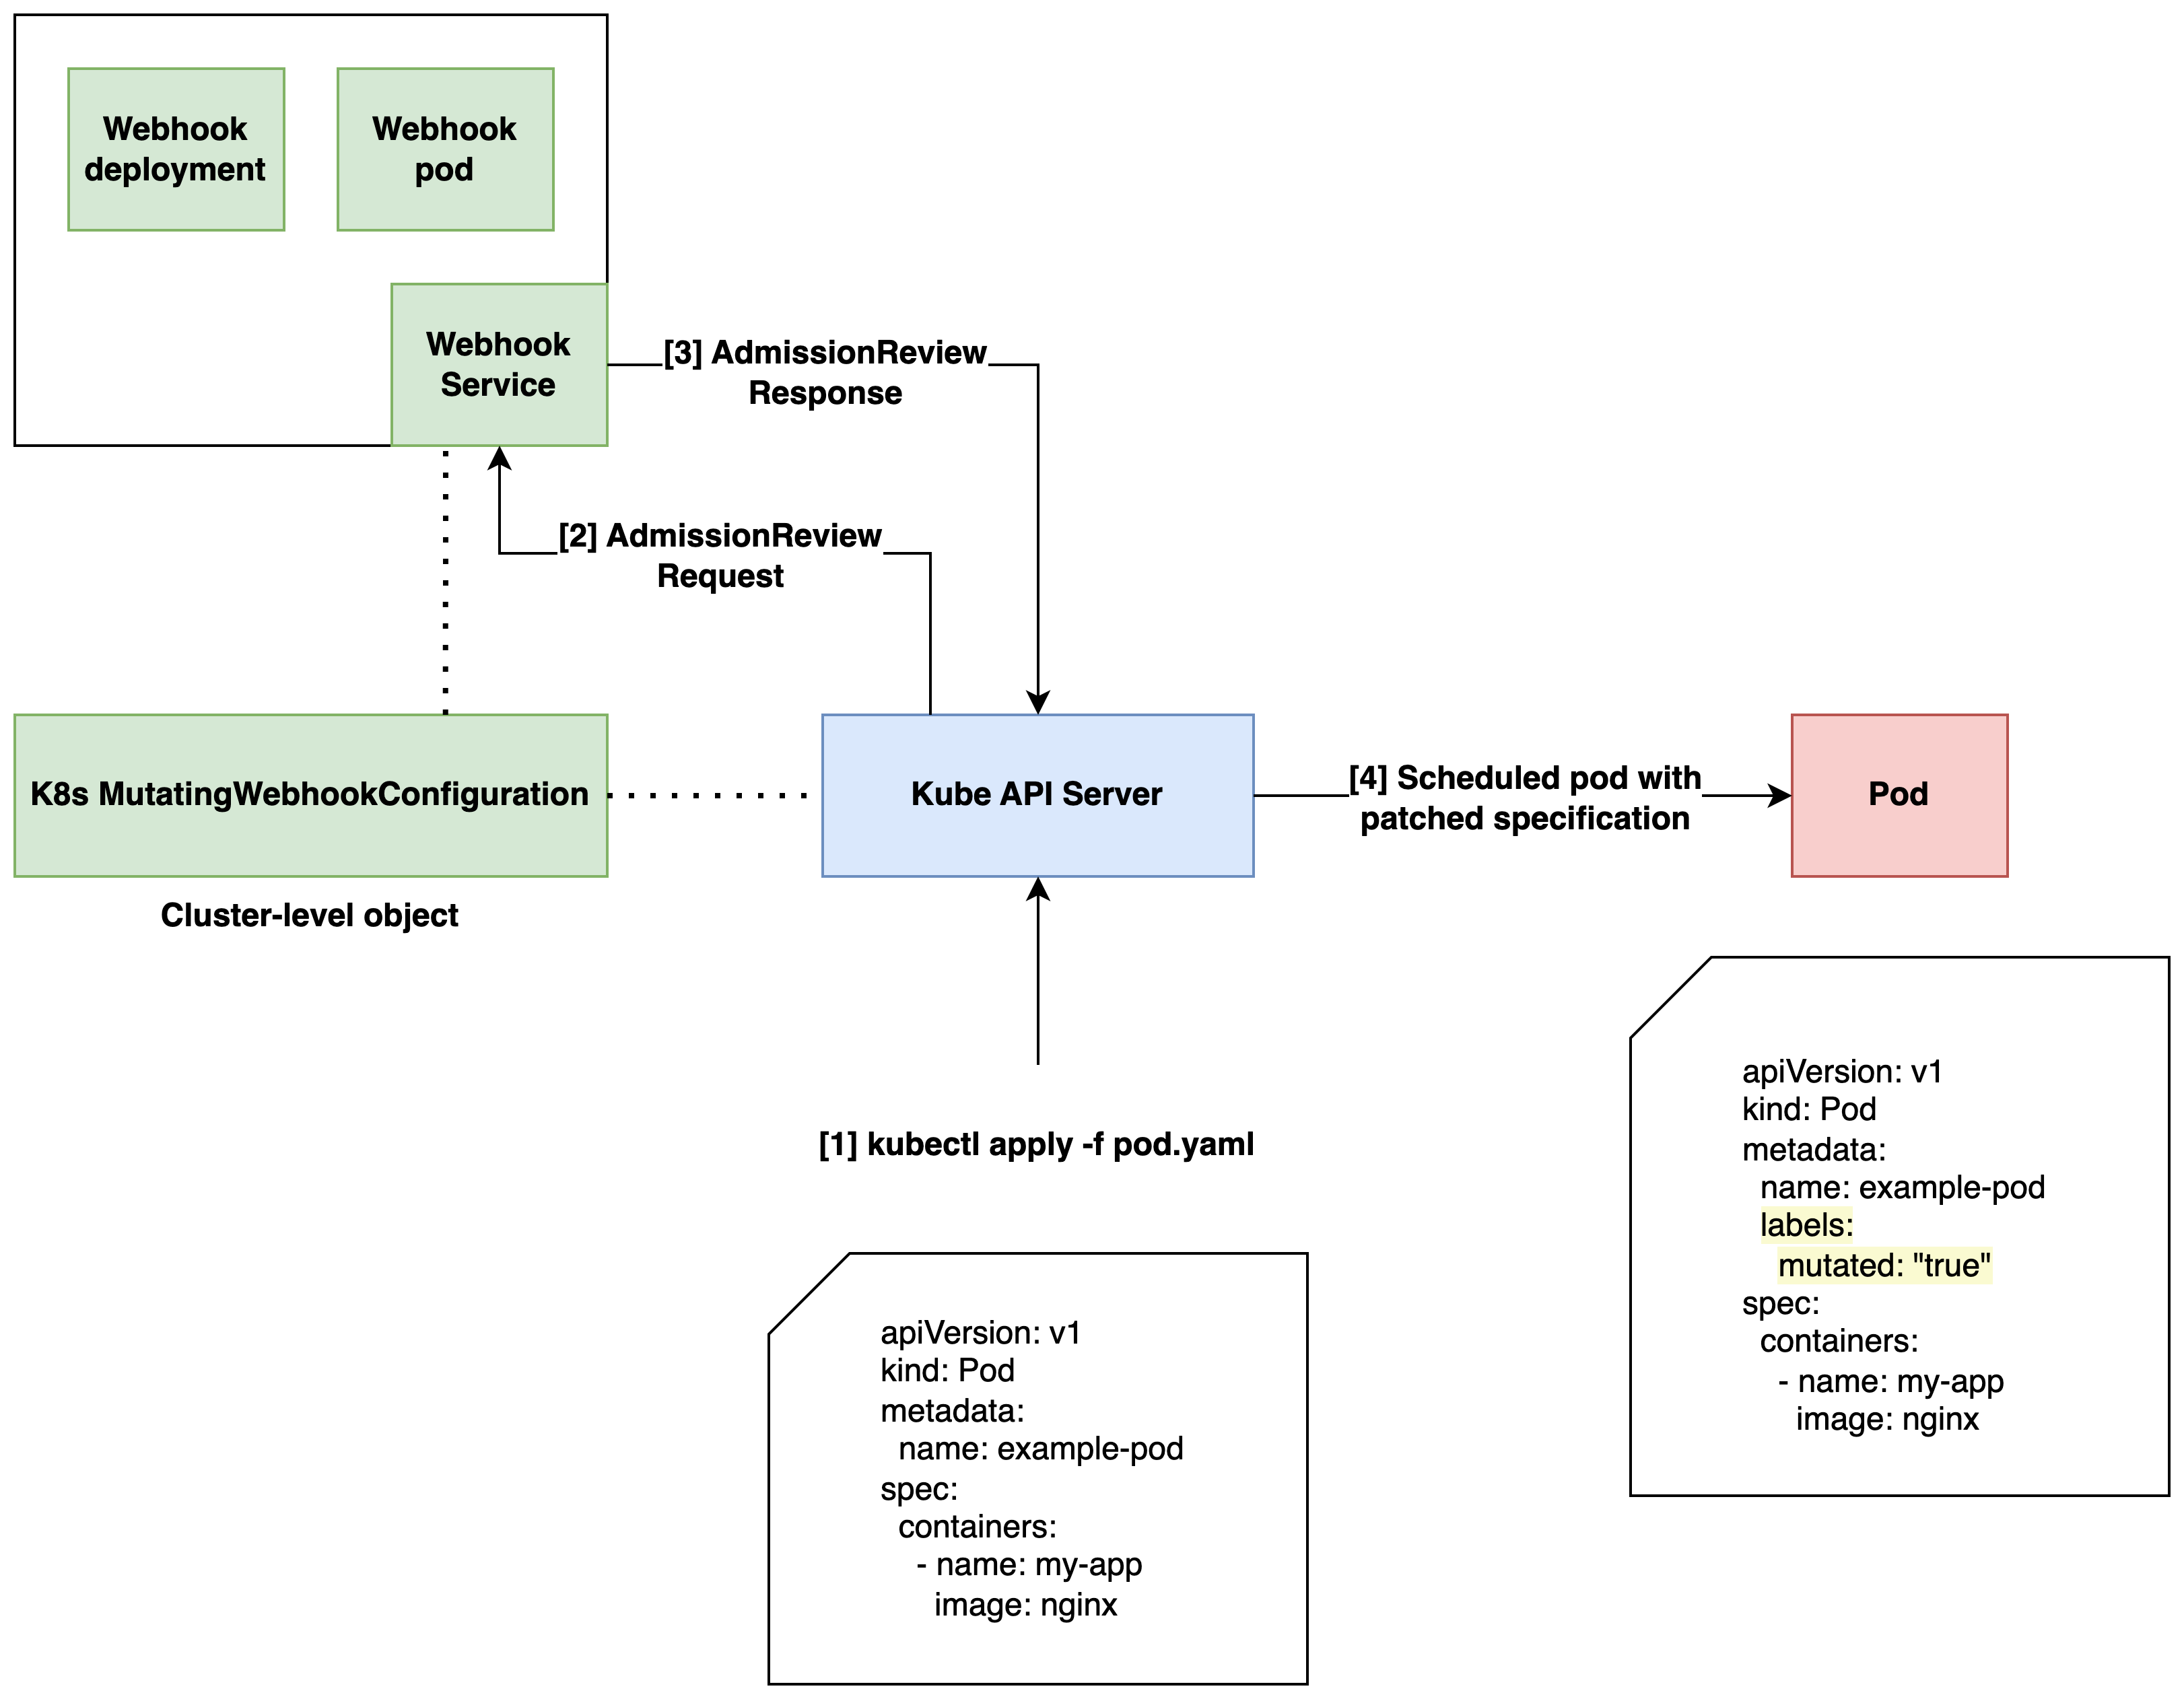
\includegraphics[width=1\linewidth]{images/k8s_webhook_example.png}
  \caption{Kubernetes Mutating Webhook example \cite{kubernetes_mutating_webhook_example}}
  \label{fig:k8s_webhook_example}
\end{figure}

In the context of our system, a \textbf{\textit{MutatingWebhookConfiguration}} is set to intercept CREATE and UPDATE Kubernetes API requests for VmTemplate Custom Resources.
In this case, the Kubernetes Mutating Webhook server that is the target of the MutatingWebhookConfiguration is Open Policy Agent (OPA).
OPA is used to assign scheduling decisions to VmTemplates based on policies. 
OPA sends back to the API server the mutation (patches) to be applied to the VmTemplate Custom Resource.
This process is further described in the next section.

\section{Open Policy Agent (OPA)}

Open Policy Agent (OPA) is an open-source general-purpose \textbf{policy engine} that enables unified policy decision-making across several types of environments \cite{opa_docs}. 
OPA provides a declarative language called \textbf{Rego} enabling a paradigm known as ``\textbf{Policy as Code}" \cite{opa_docs}.
Open Policy Agent can be integrated as a sidecar container, host-level daemon, or library to perform policy decisions for a plethora of use cases: \textbf{Kubernetes admission control}, CI/CD pipelines, container images, microservices, etc.\cite{opa_docs}. 
In the context of our system, OPA and the Policy-as-Code paradigm are mainly leveraged to define \textbf{policies for workload scheduling}: encoding the output of a \textbf{scheduling decision} coming from an external GreenOps Scheduler and ensuring compliance with \textbf{additional policies} related to latency requirements and legal constraints (QoS, data residency, etc.).
In particular, OPA assumes the role of a \textbf{Kubernetes Mutating Webhook server} to apply scheduling decisions to VmTemplate Custom Resources based on policies.

\subsection{Policy as Code paradigm}

According to AWS, Policy-as-Code (PaC) is a software automation approach which is similar to Infrastructure-as-Code (IaC) \cite{pac_aws}. 
PaC helps assess company system configurations and validate compliance requirements through software automation \cite{pac_aws}. 
The perceived value of this type of automation in the software development lifecycle has grown significantly in modern enterprises. 
This large adoption is probably driven by the inherent consistency and reliability it provides, ensuring standardized enforcement of policies and reducing human error, as what happened with the IaC approach \cite{pac_aws}.

OPA's generic definition of policy is: ``\textit{A policy is a set of rules that governs the behavior of a software service}" \cite{opa_philosophy}. OPA provides a high-level declarative language called \textbf{Rego} to define policies in a flexible manner. 
One of OPA's key strengths is its \textbf{domain-agnostic design}, allowing it to enforce policies across various systems and environments. 
This makes it highly adaptable to different use cases, ranging from access control to infrastructure security. 
Some representative examples of policies that OPA can enforce include:

\begin{itemize}[itemsep=0.2pt, topsep=1pt] \item[$\bullet$] Restricting which image registries can be used for deploying new Pods in a Kubernetes cluster.
\item[$\bullet$] Controlling whether a specific user is permitted to perform delete operations on certain resources.
\item[$\bullet$] Enforcing network security policies, such as blocking external access to sensitive services.
\item[$\bullet$] Ensuring infrastructure compliance, for example, by verifying that new cloud resources to be provisioned follow predefined security configurations.
\item[$\bullet$] Enforcing that new deployed servers must have the prefix ``server-" in their name.
\end{itemize}

Another interesting example is the use of OPA for \textbf{compliance automation for AWS infrastructure} \cite{10612535}. 
In this case, OPA is used by the authors as a step in a CI/CD pipeline to enforce compliance policies on AWS infrastructure represented with the Infrastructure as Code (IaC) tool CloudFormation \cite{10612535}.
Therefore, the use cases covered span from role-based access control to container image security and beyond.
\newline

Another important aspect of OPA is that it effectively \textbf{decouples} policy decision-making from policy enforcement \cite{opa_docs}.
In practice, this means that when a software module needs to make a policy decision, it queries OPA, supplying relevant data as input. 
In other words, policy decisions are \textbf{offloaded} to OPA rather than being hardcoded within individual services. 
This approach offers several key advantages \cite{opa_docs}:
\begin{itemize}[itemsep=0.2pt, topsep=1pt]
  \item[$\bullet$] \textbf{Centralized policy management}: policies are defined in a single location, ensuring uniform enforcement across all services of an organization.
  \item[$\bullet$] \textbf{Improved maintainability}: updating policies does not require modifying, recompiling or redeploying application code, reducing complexity, errors and deployment overhead.
  \item[$\bullet$] \textbf{Greater flexibility}: policies can be dynamically updated (e.g., with CI/CD approaches) based on evolving security and compliance requirements. 
  \item[$\bullet$] \textbf{Scalability}: since OPA and application modules are not tightly coupled.
\end{itemize} 

\subsection{OPA architecture overview}

As mentioned in the introduction to this section, one common approach to integrating OPA into a software system is by deploying it as a host-level daemon. 
The latter is essentially a lightweight server that processes policy queries via HTTP requests. 
This setup allows services to offload policy decision-making to OPA in a scalable and efficient manner since the two entities are not tightly coupled.

A standard OPA deployment consists of three main components:

\begin{enumerate}[itemsep=0.2pt, topsep=1pt]
  \item \textbf{OPA Server}: The core service that evaluates policy queries and returns decisions based on defined rules, contextual data and input data.
  \item \textbf{OPA Policies}: Rules written in the Rego language that define the logic to be enforced.
  \item \textbf{Data}: Optional contextual information, typically structured in JSON format, that policies use to make informed decisions along with input data.
\end{enumerate}

To facilitate deployment and management, Rego policies and associated contextual data are packaged into \textbf{policy bundles}, as described in section \ref{sec:opa_policies}. These bundles enable version-controlled, centralized policy distribution, ensuring consistency and maintainability across distributed environments. \newline


\begin{figure}[htb]
\centering
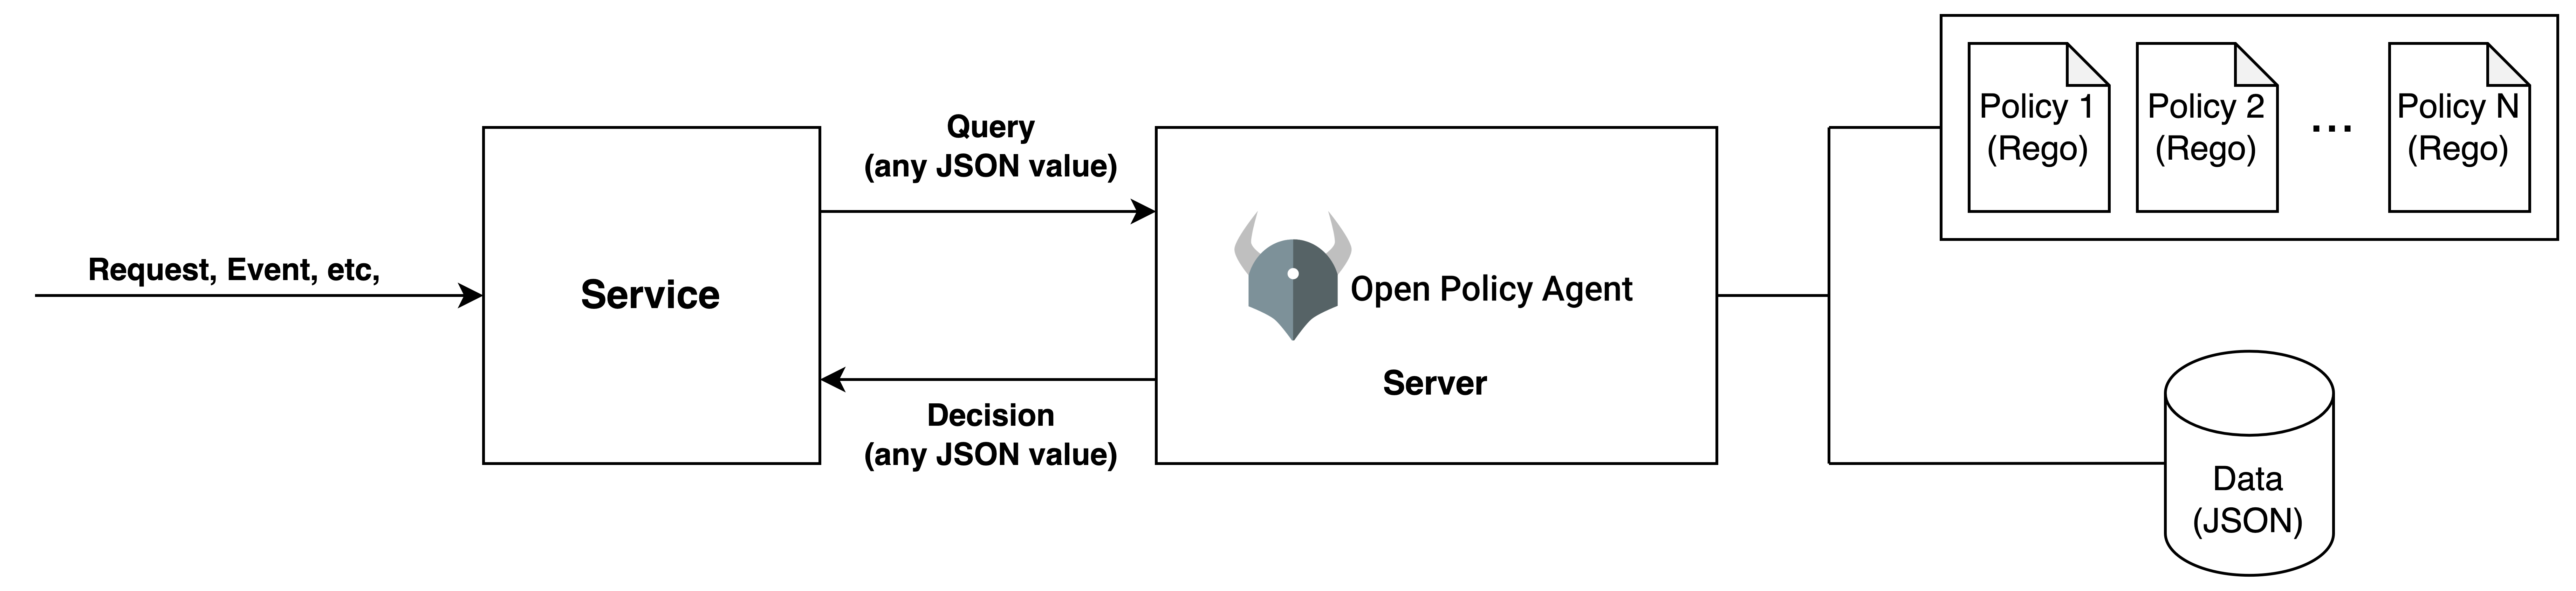
\includegraphics[width=1\linewidth]{images/OPA.png}
\caption{OPA architecture}
\label{fig:opa_architecture}
\end{figure}


OPA accepts arbitrary structured data as input and can generate arbitrary structured data as output. 
This flexibility allows OPA to be used in a wide range of use cases, as described above.

\subsection{OPA and external data sources}
\label{sec:opa_external_data}

In order to get data from external sources, OPA provides several options that can be chosen based on size and frequency of update \cite{opa_external_data}.
For the use case of this work, external data to be pulled is the \textbf{scheduling decision} from the GreenOps Scheduler in a synchronous way.
The most suitable option is to \textbf{pull data during policy evaluation} since scheduling decisions must be made in real-time.
The data is pulled from the GreenOps Scheduler (effectively a HTTP server) with the use of the OPA built-in function ``\textit{http.send()}'' which can be used to send HTTP requests to arbitrary endpoints just like a ``curl'' command in a shell script \cite{opa_external_data}.
The listings \ref{lst:scheduler_req} and \ref{lst:opa_external_data} respectively show an example of a HTTP request to the GreenOps Scheduler and how the OPA external data pull is implemented in Rego.

\begin{lstlisting}[language=sh, caption={GreenOps scheduler HTTP request example}, label={lst:scheduler_req}]
#!/bin/bash
curl -X POST -H "Content-Type: application/json" \
  -d '{
      "number_of_jobs" : 1,
      "eligible_regions": ["FR", "IT", "FI"],
      "deadline": "2025-06-09T10:00:00",
      "duration": 6,
      "cpu": 4,
      "memory": 8,
      "req_timeout": 180
 }' http://greenops-scheduler.greenops-scheduler-system.svc.cluster.local/scheduling

# Response: 
# {"scheduling_location":"FR","scheduling_time":"2025-02-06T17:42:11Z"}
\end{lstlisting}

\begin{lstlisting}[language=rego, caption={OPA external data pull}, label={lst:opa_external_data}]
scheduler_url := opa.runtime().env.SCHEDULER_URL

scheduling_details := http.send({
	"method": "POST",
	"url": scheduler_url,
	"body": {
		"number_of_jobs": 1, # currently only one job (workload (VM)) can be scheduled at a time
		"eligible_regions": eligible_electricity_maps_regions,
		"deadline": deadline,
		"duration": duration, 
		"cpu": cpu,
		"memory": memory,
		"req_timeout": 10 # seconds, scheduler wants to know the timeout to tune the execution time of the optimization
	},
	"timeout": "10s",
	"headers": {
		"Content-Type": "application/json"
	},
	"max_retry_attempts": 3,
})
\end{lstlisting}

\subsection{OPA integration with Kubernetes}

In the context of Kubernetes Admission Control mechanism, policy enforcement is handled by the \textbf{Kubernetes API server} itself. 
OPA makes the policy decisions when queried by the admission controller, but the actual enforcement (namely allowing, denying, modifying requests) is executed by Kubernetes' built-in admission control mechanisms. 
This is effectively one of the core design principles of OPA: to provide policy decisions to external systems, which then enforce the decisions based on their own logic \cite{opa_kubernetes_primer}.
This workflow is represented in figure \ref{fig:webhook_opa} where the \textbf{AdmissionReview request} and \textbf{AdmissionReview response} are respectively input and output of the whole OPA section. 
The API Server sends the entire Kubernetes object in the webhook request to OPA \cite{opa_kubernetes_primer}.
The Kubernetes API server will use the received AdmissionReview response for its decision. \\
%\cite{opa_philosophy}
% https://www.openpolicyagent.org/docs/latest/kubernetes-tutorial/

\begin{figure}[htb]
\centering
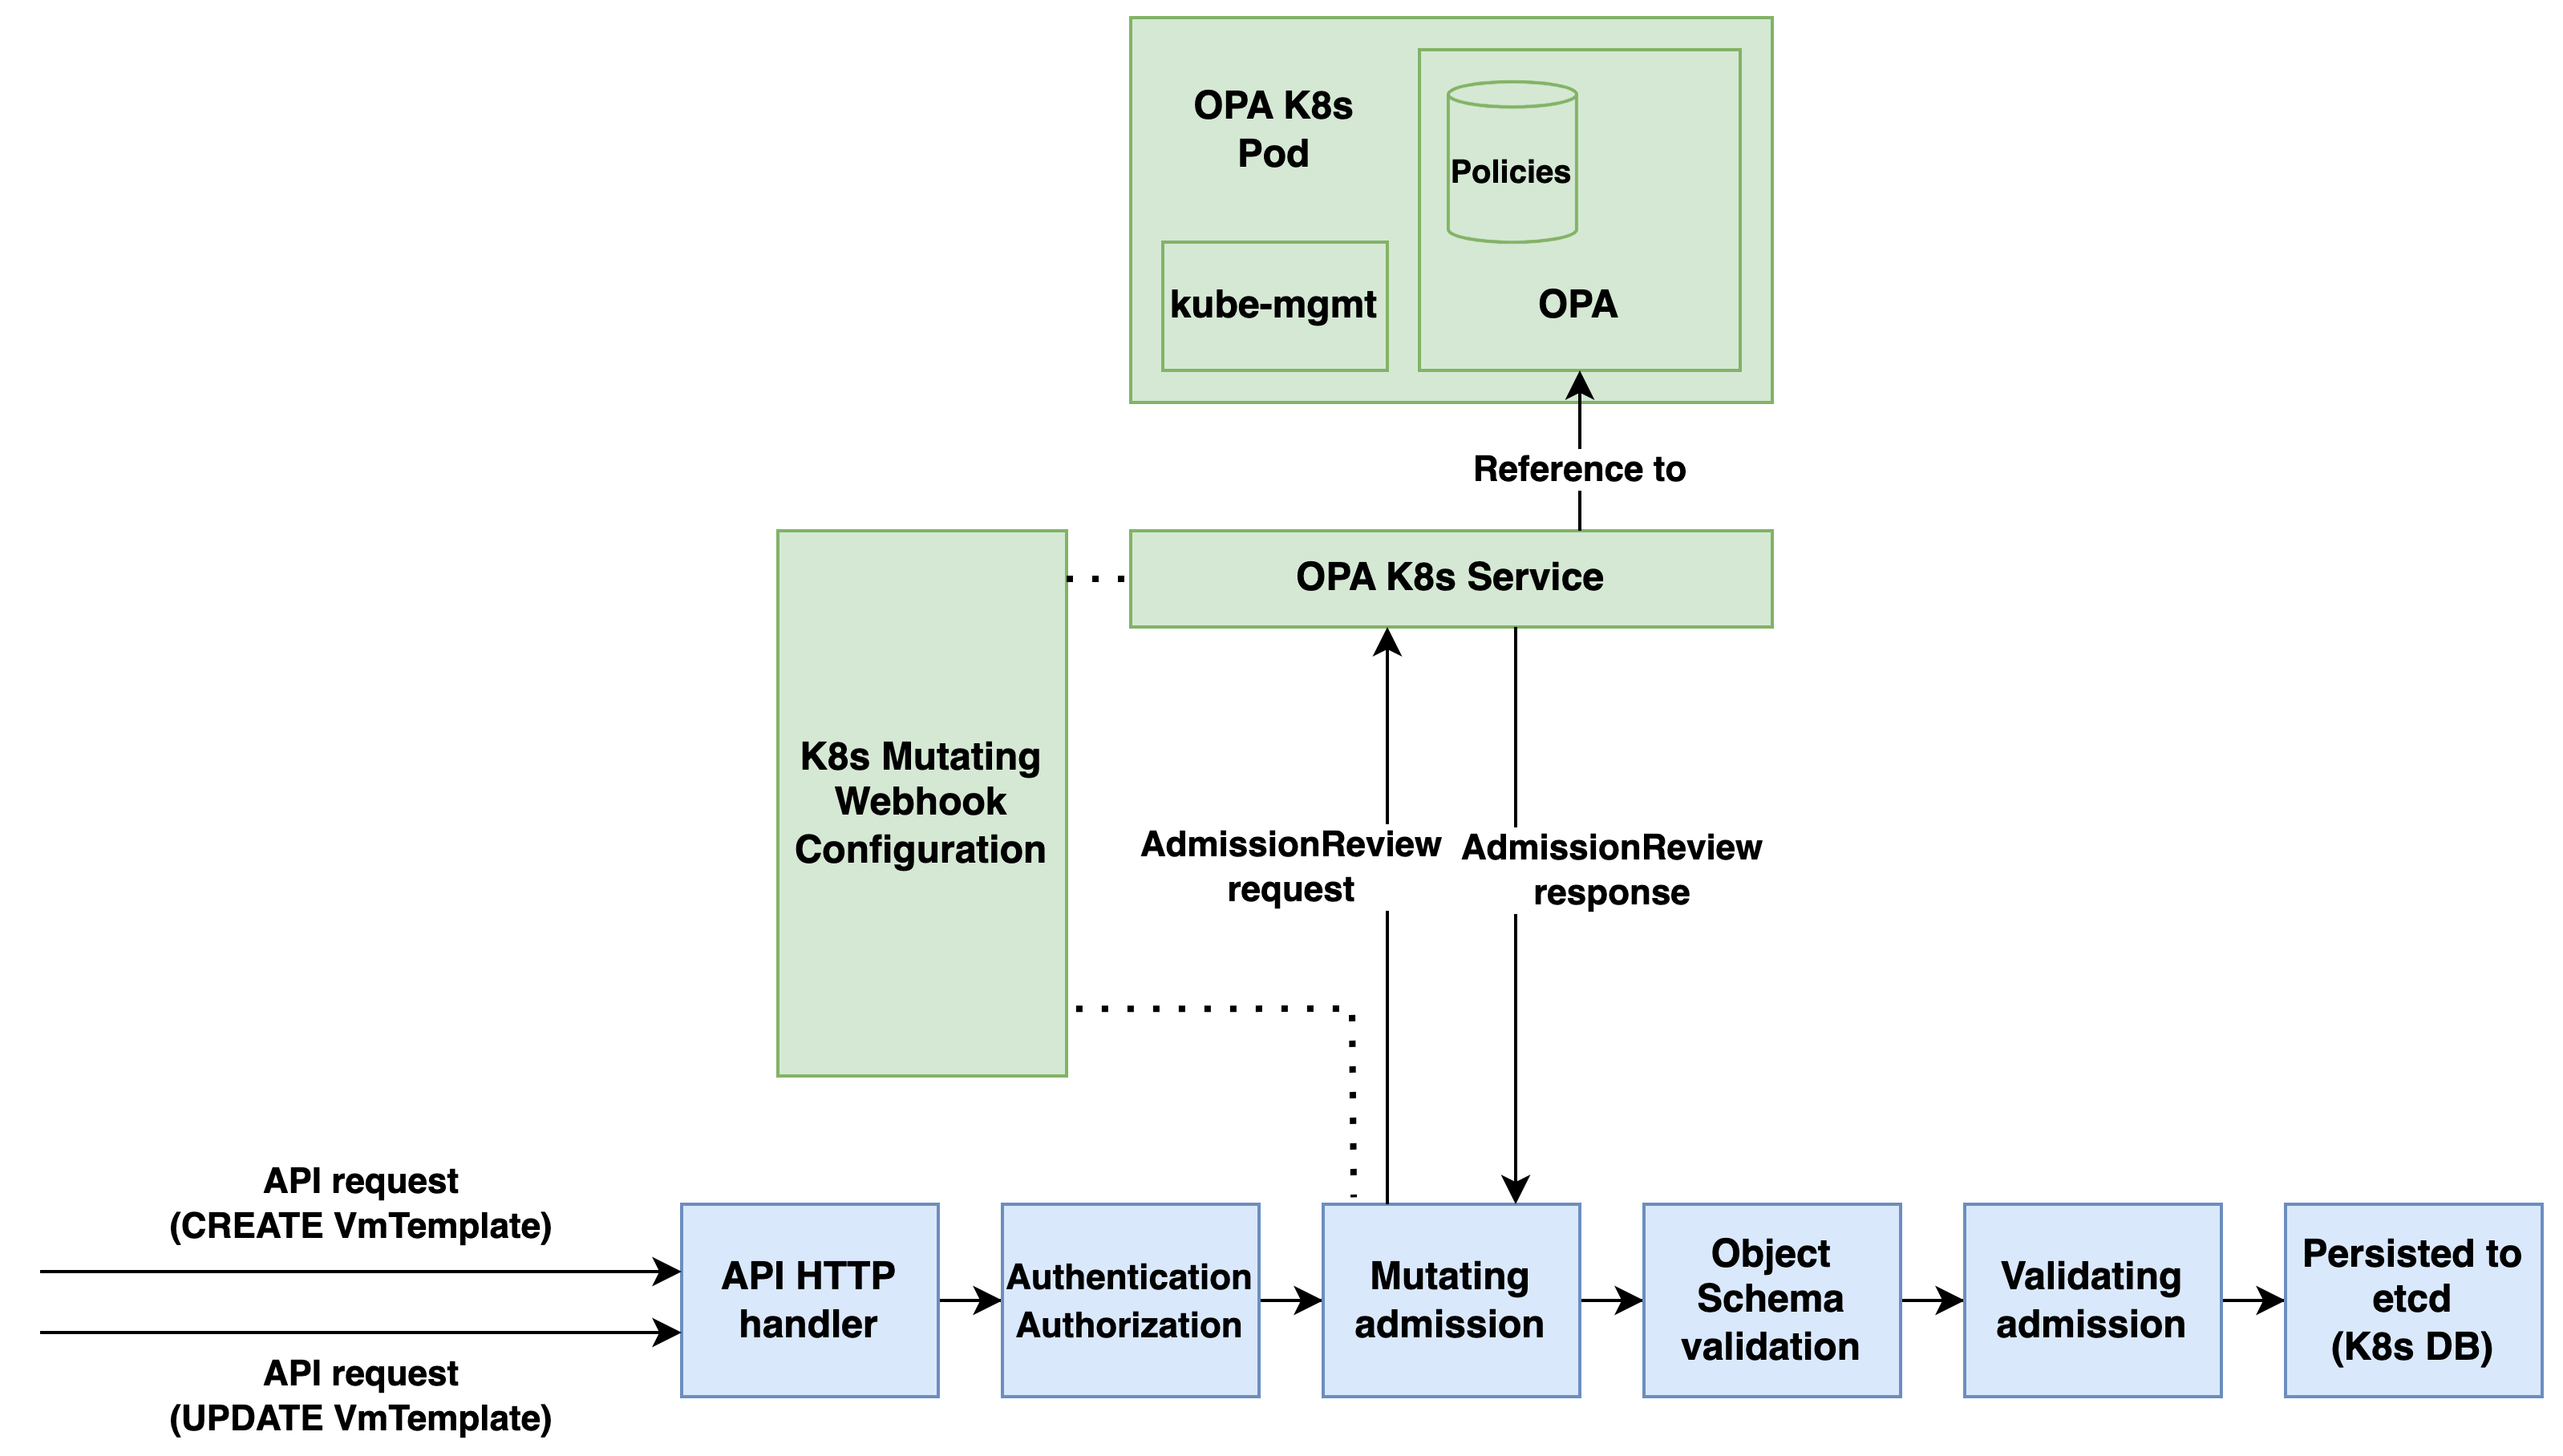
\includegraphics[width=1\linewidth]{images/webhook.png}
\caption{Kubernetes mutating webhook and OPA integration}
\label{fig:webhook_opa}
\end{figure}

In a Kubernetes deployment, an \textbf{OPA server Pod} typically consists of the following containers:
\begin{itemize}[itemsep=0.2pt, topsep=1pt]
  \item[$\bullet$] OPA server container
  \item[$\bullet$] \textbf{kube-mgmt} container \\
\end{itemize} 

The kube-mgmt container functions as a \textbf{sidecar container} within a Kubernetes Pod. The sidecar container pattern is a common Kubernetes design paradigm in which auxiliary containers run alongside the main application container within the same Pod. These additional containers serve to enhance, extend, or support the primary application's functionality without modifying its core logic \cite{sidecar_containers}. 
The primary responsibility of kube-mgmt is to replicate Kubernetes resources into the OPA instance (OPA container). This operation is essential for OPA to access and evaluate policies based on real-time cluster state, enabling dynamic policy enforcement. By synchronizing these resources, kube-mgmt ensures that OPA has an up-to-date view of relevant Kubernetes objects.
This is especially useful to enforce policies that deals with naming conflicts, where OPA needs to check existing names in the cluster for the decision \cite{kube-mgmt}.
Additionally, it allows for loading policies directly from the Kubernetes cluster by retrieving them in the form of ConfigMaps. This feature is particularly useful when policies need to be dynamically updated based on the current state of the cluster \cite{kube-mgmt}. However, in the system described in this thesis, this latter feature is not employed in the current implementation as we are using policy bundles for policy distribution.

In the current system configuration, the kube-mgmt container is deployed to facilitate resource replication, ensuring that Kubernetes resources, namely VmTemplate resources, are synchronized with the OPA instance. 
However, at present, no policy requires interrogation of VmTemplate resources that are already present in the system.
Looking ahead, future policies could leverage VmTemplate resource information to enforce naming conflict resolution, quota management, or additional constraints.

\subsection{OPA policies}
\label{sec:opa_policies}

%example of a policy:
%(https://www.openpolicyagent.org/docs/latest/kubernetes-primer/)

As OPA official documentation describes, when the Kubernetes AdmissionReview request from the webhook arrives, it is bound to the \textbf{OPA input document} and generates the default, ``root", decision: \textit{system.main} \cite{opa_docs}.
The root policy, in the case of Kubernetes admission control, is responsible for generating the AdmissionReview response in accordance with the Kubernetes API specifications. 
Indeed, it is the duty of the policy developer to write Rego code that produces a \textbf{well-formed AdmissionReview response}, ensuring that the OPA server can then correctly communicate its decision to the Kubernetes admission controller \cite{opa_docs}.
OPA policies are compiled before being evaluated, and any errors that occur during compilation are reported back to the caller.
An example of these errors is when there are merge errors on contextual data \cite{opa_docs}.
For the purpose of this thesis, it is deemed useful to show one of the simplest and common example of a OPA policy in the \textbf{Kubernetes admission control context}. 
That is: to ensure all images for Kubernetes Pods come from a trusted registry, namely \textit{unitn.it}.
It is important to note that, in this case, due to the simplicity of the policy, no additional contextual data in JSON format is required while in a standard scenario, data is used to provide additional context to the policy evaluation process. \newline

Listing \ref{lst:rego_policy_example} shows the Rego policy that enforces the rule described above while listing \ref{lst:rego_root_policy} shows the root policy that generates the AdmissionReview response.
Listings \ref{lst:admission_review_request} and \ref{lst:admission_review_response} show respectively an example of an AdmissionReview request and response. \newline

\begin{lstlisting}[language=Rego, caption={Rego policy for Pods registry}, label=lst:rego_policy_example]                              
deny contains msg if {                                                      
    input.request.kind.kind == "Pod"                                        
    image := input.request.object.spec.containers[_].image                  
    not startswith(image, "unitn.it/")                                     
    msg := sprintf("image '%v' comes from untrusted registry", [image])     
}
\end{lstlisting}

\begin{lstlisting}[language=Rego, caption={Rego ``root" policy (system.main)}, label=lst:rego_root_policy]
package system

import data.kubernetes.admission

main := {
	"apiVersion": "admission.k8s.io/v1",
	"kind": "AdmissionReview",
	"response": response,
}

default uid := ""

uid := input.request.uid

response := {
	"allowed": false,
	"uid": uid,
	"status": {"message": reason},
} if {
	reason := concat(", ", admission.deny)
	reason != ""
}

else := {"allowed": true, "uid": uid}
\end{lstlisting}

\lstset{style=jsonstyle}
\begin{lstlisting}[caption={AdmissionReview request}, label={lst:admission_review_request}]
{
    "apiVersion": "admission.k8s.io/v1",
    "kind": "AdmissionReview",
    "request": {
        "kind": {
            "group": "",
            "kind": "Pod",
            "version": "v1"
        },
        "object": {
            "metadata": {
                "name": "myapp"
            },
            "spec": {
                "containers": [
                    {
                        "image": "bitnami/node:22",
                        "name": "nodejs"
                    }
                ]
            }
        }
    }
}
\end{lstlisting}

\lstset{style=jsonstyle}
\begin{lstlisting}[caption={AdmissionReview response}, label={lst:admission_review_response}]
{
    "apiVersion": "admission.k8s.io/v1",
    "kind": "AdmissionReview",
    "response": {
        "allowed": false
        "status": {
            "message": "image 'bitnami/node:22' comes from untrusted registry"
        }
    }
}
\end{lstlisting}

Therefore, in this specific case, the creation of the Kubernetes Pod will be \textbf{denied}. 
OPA is responsible for \textbf{decision-making}, determining that the request do not complies with the defined policies, while the Kubernetes API server, using the AdmissionReview response generated by OPA, handles \textbf{policy enforcement}, effectively rejecting the CREATE request since it violates the specified rules.

\subsection{OPA policy bundles}
\label{sec:opa_bundles}

An OPA policy bundle is a collection of policies and optional associated contextual data. More precisely, a bundle is a standardized way to package policies, facilitating version control and distribution \cite{opa_bundles}. As a matter of fact, a single policy bundle can be potentially used by multiple OPA instances.
A policy bundle mainly consists of:
\begin{itemize}[itemsep=0.2pt, topsep=1pt]
  \item[$\bullet$] \textbf{Rego policy files} defining the logic.
  \item[$\bullet$] \textbf{Data files} (in JSON or YAML format) containing contextual information required for policy evaluation (e.g., cloud region mappings).
\end{itemize} 

Policy bundles can be distributed through a variety of mechanisms such as remote HTTP servers (e.g., NGINX) and object storage services (e.g., Amazon S3, Google Cloud Storage, Azure Blob Storage) \cite{opa_bundles}.
One of the most convenient approaches is packaging policy bundles as \textbf{OCI (Open Container Initiative) images} \cite{oci} and this is the approach adopted in the system described in this thesis.
Once packaged as OCI images, policy bundles can be pulled by OPA servers from a container registry at predefined and configurable time intervals. 
This allows policy updates to be deployed in OPA \textbf{without requiring manual intervention} or \textbf{service restarts}, ensuring that enforcement mechanisms remain up to date with the latest compliance requirements identified and implemented by the organization. 
This is crucial for instance when dealing with \textbf{critical security policies} that need to be updated frequently, maybe in response to the discoveries of new CVEs. 
In the context of our system, such timely updates are not essential but the OPA is designed to be able to handle them if needed.
To ensure continuous policy enforcement while maintaining high operational efficiency, a CI/CD approach is adopted for policy management in the context of our system.
As a matter of fact, policies are maintained in a \textbf{version-controlled hosted repository} (i.e., on GitHub), where updates like tagging (``git tag'') trigger an automated pipeline (e.g., using GitHub Actions) responsible for building, packaging into a OCI image, and publishing the policy bundle to a container registry (e.g., Docker Hub).
One of the major advantages of this approach is the ability to dynamically update policies without requiring OPA Pods to restart as there is an \textbf{hot-reload} of policies done at application level by OPA (``loaded on the fly'') \cite{opa_bundles}. 
This is particularly useful in production environments where service availability is critical and downtime must be minimized. 
The overall process of policy distribution adopted and implemented in our system is illustrated in figure \ref{fig:opa_bundles}.

\begin{figure}[H]
\centering
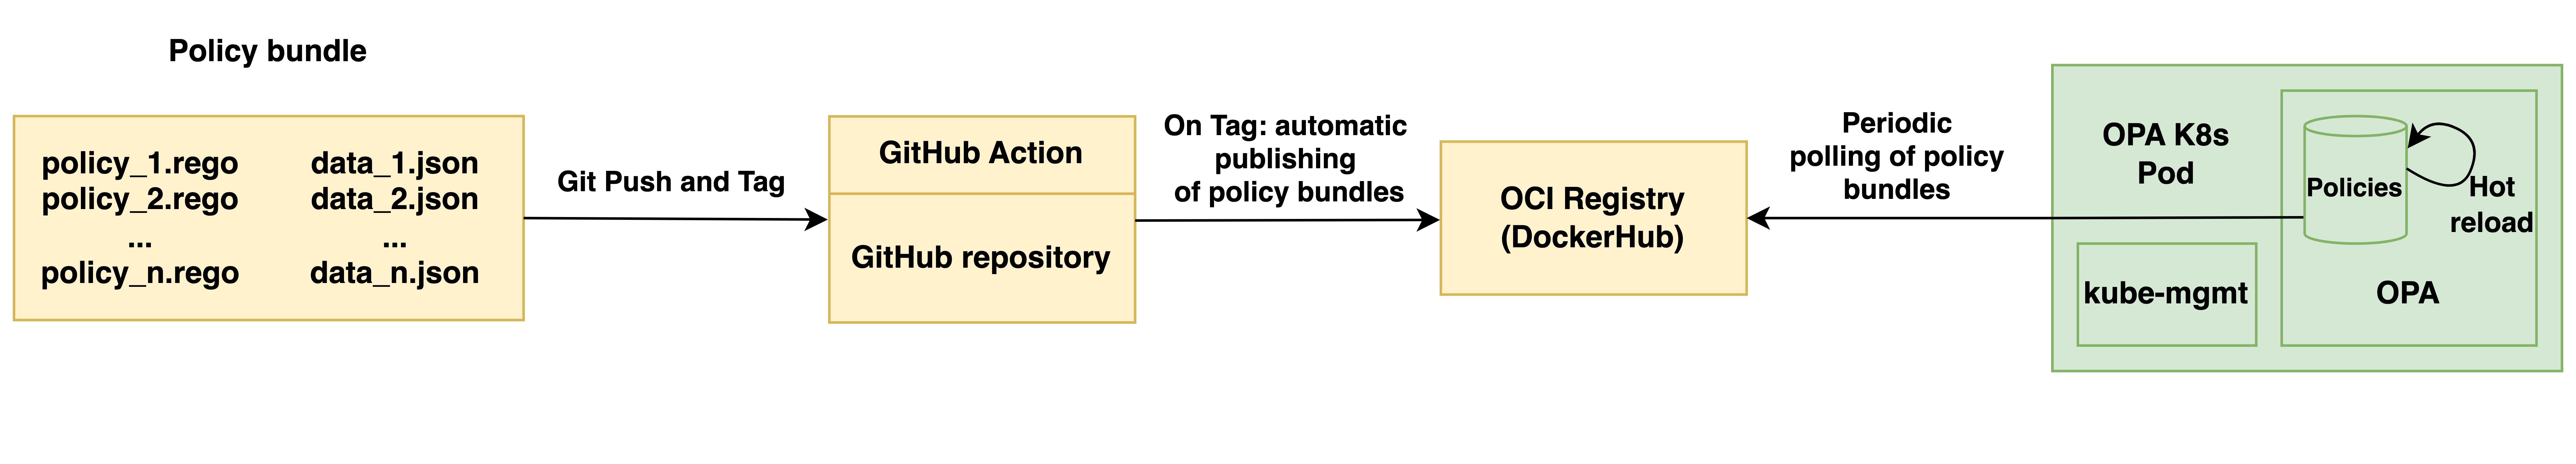
\includegraphics[width=1\linewidth]{images/opa_bundles.png}
\caption{OPA policy bundles}
\label{fig:opa_bundles}
\end{figure}

By leveraging OCI images for policy distribution and implementing fully automated CI/CD pipelines, this methodology ensures that policy enforcement remains consistent, up to date, and highly available across all OPA instances. 
This approach aligns with modern and standard DevOps practices, enabling organizations to maintain a high level of security and compliance without compromising operational efficiency.

\subsection{Latency policy}

A representative example of a policy aligned with Service Level Objectives (SLOs) or Service Level Agreements (SLAs) is the latency policy described in this section.
Given an \textbf{origin region} and a \textbf{maximum latency threshold} (expressed in milliseconds), the objective is to determine a \textbf{set of eligible regions} where the inter-regional latency between the origin and each region in the set is equal to or below the specified threshold.
Enforcing such constraints helps mitigate the so-called ``\textbf{black hole phenomenon}" in the GreenOps use case, where all virtual machines (VMs) would otherwise be scheduled in a region with generally low carbon intensity, without considering additional constraints or performance requirements. By incorporating similar performance-aware policies, organizations can achieve a balance between environmental impact, performance, and service reliability.
The proposed flexible system enables organizations to fine-tune these factors according to their specific requirements or those of their users. 
This policy demonstrates the flexibility of OPA in handling diverse compliance scenarios. It is the responsibility of the policy developer to design an appropriate strategy for encoding relevant information into \textbf{well-structured JSON data models}, e.g., a latency matrix. Proper structuring ensures efficient policy evaluation, maintainability and extendability.

Figure \ref{fig:latency_matrix} illustrates an small example (4 regions subset) of a latency matrix, where each cell represents the latency between two regions. The matrix can be encoded in JSON format as illustrated in listing \ref{lst:latency_matrix_example}, allowing for easy integration with OPA policies. The ``Latency policy'' then uses this matrix to determine eligible regions based on the origin region and maximum latency threshold.

\begin{figure}[H]
  \centering
  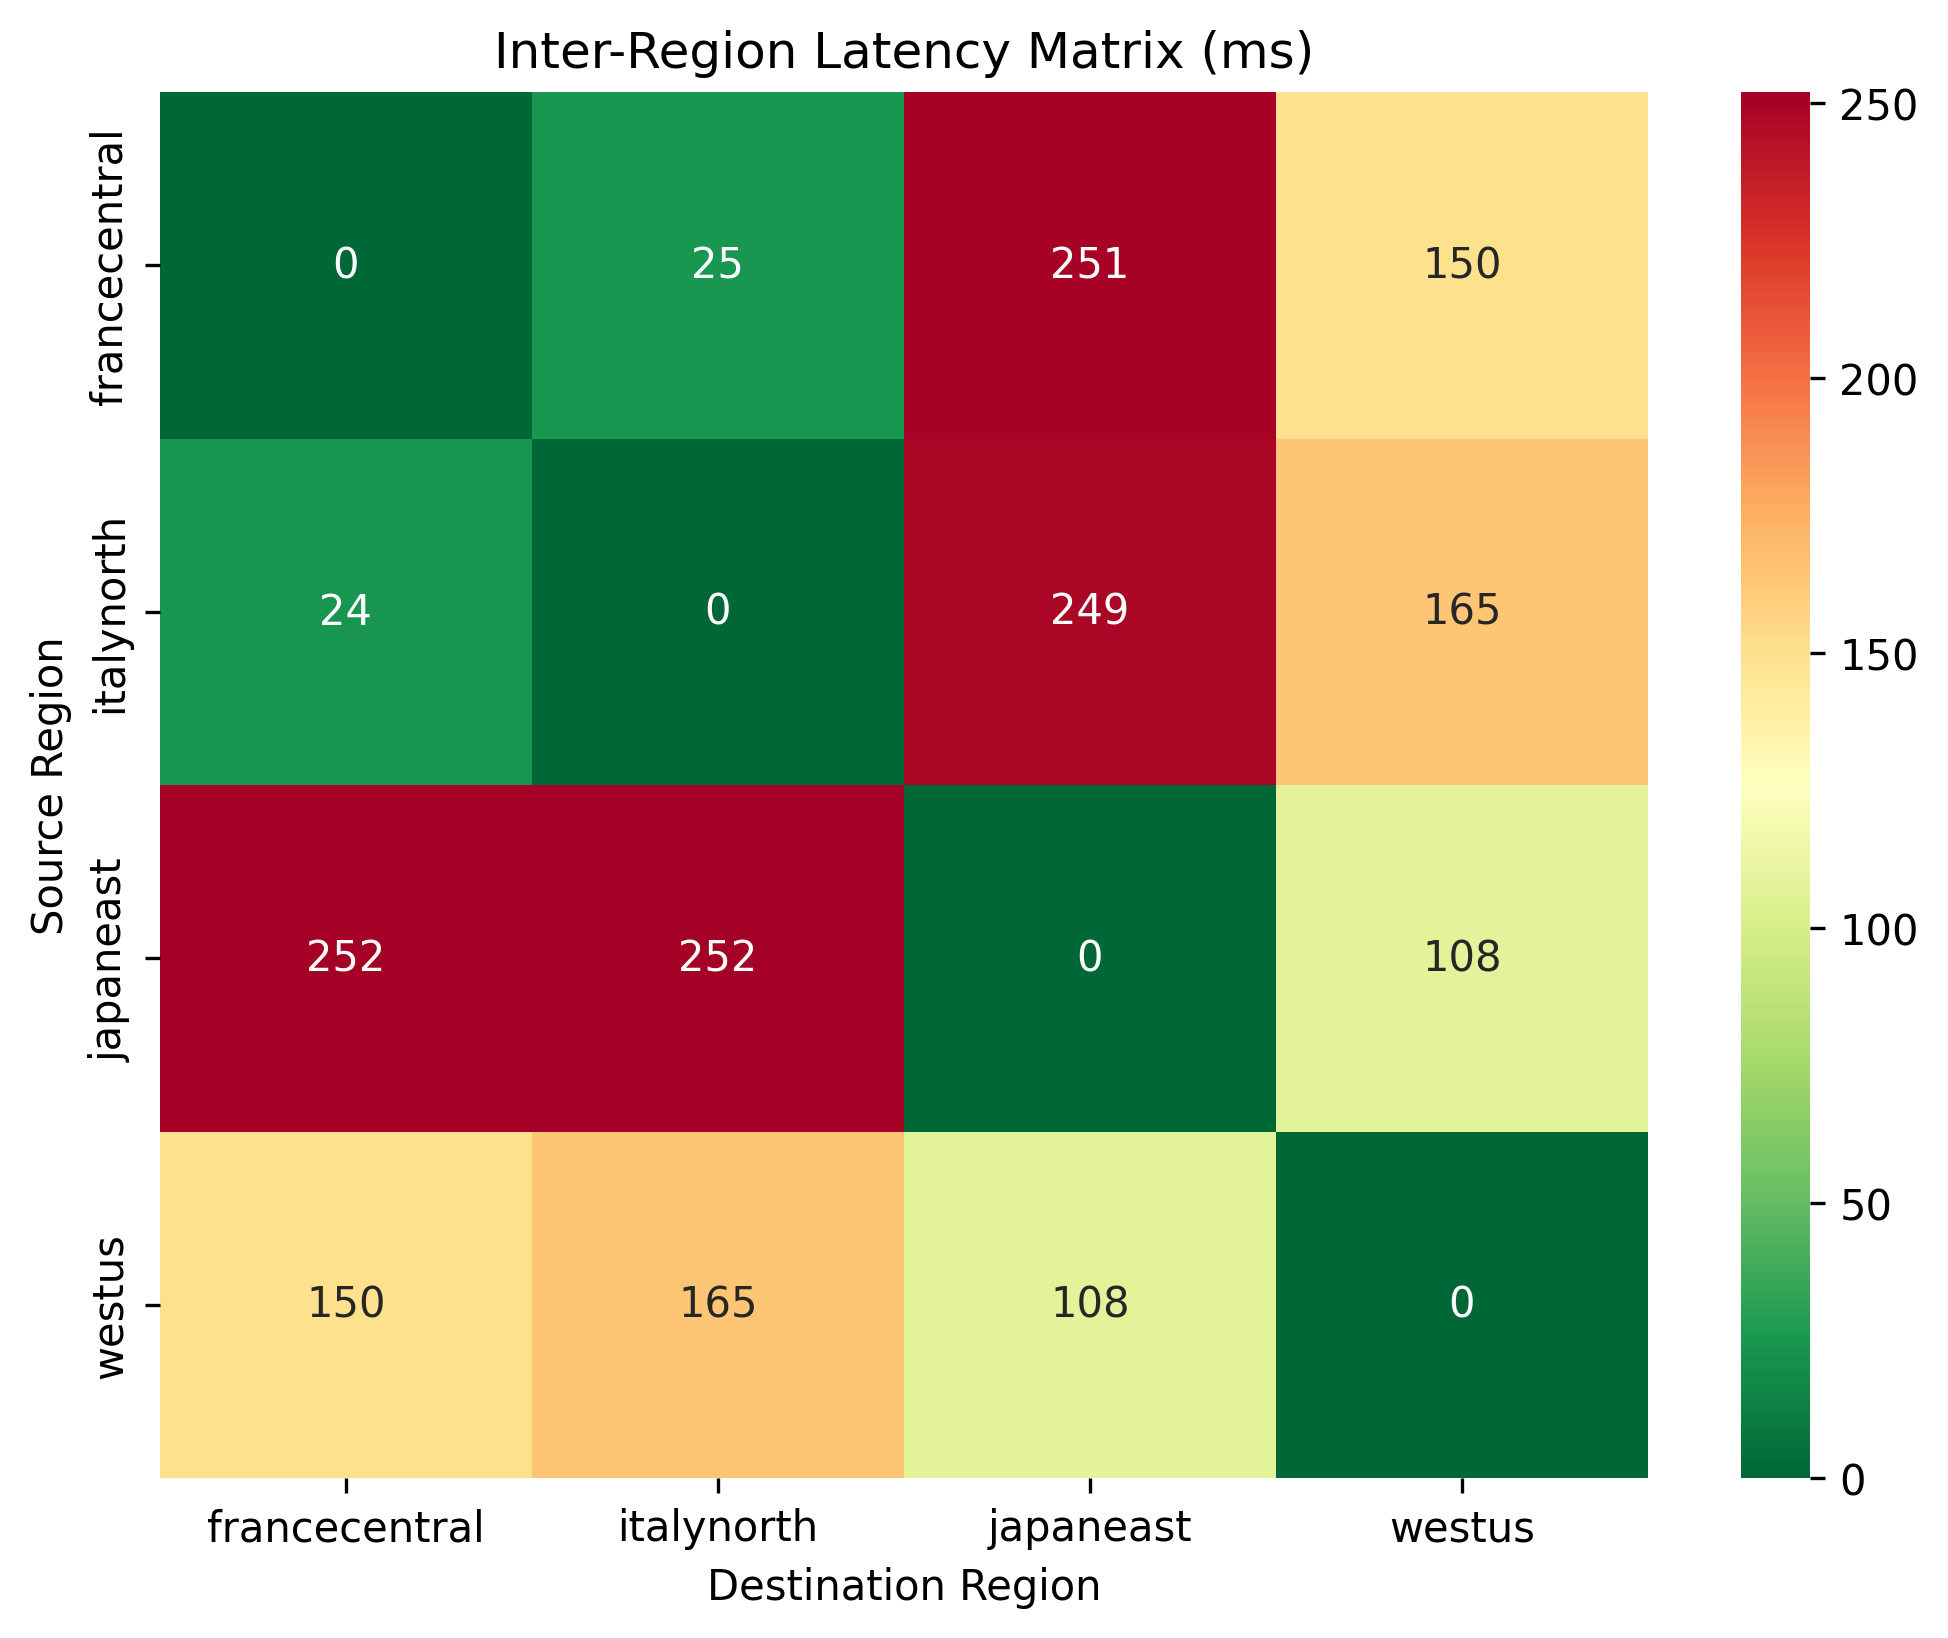
\includegraphics[width=0.575\linewidth]{images/latency_heatmap.png}
  \caption{Latency matrix example (Azure regions subset)}
  \label{fig:latency_matrix}
\end{figure}

\lstset{style=jsonstyle}
\begin{lstlisting}[caption={Latancy matrix example encoded in JSON format}, label={lst:latency_matrix_example}]
{
  "italynorth": {
      "italynorth": 0,
      "japaneast": 249,
      "francecentral": 24,
      "westus": 165
  },
  "japaneast": {
      "italynorth": 252,
      "japaneast": 0,
      "francecentral": 252,
      "westus": 108
  },
  "francecentral": {
      "italynorth": 25,
      "japaneast": 251,
      "francecentral": 0,
      "westus": 150
  },
  "westus": {
      "italynorth": 165,
      "japaneast": 108,
      "francecentral": 150,
      "westus": 0
  }
}

\end{lstlisting}

For what concern data sources, cloud-specific inter-regional latency data were obtained in different ways for each cloud provider.
Microsoft Azure provides monthly ``Percentile P50 round trip times'' between Azure regions in its documentation \cite{azure_network_latency}. 
This data was automatically scraped, merged and used to build the latency matrix for Azure regions.
For AWS a similar approach was used, but the data was obtained from a third-party website that provides latency data between AWS regions calculating using AWS Lambda functions \cite{cloudping}.
For Google Cloud Platform, no official data was found, so the latency matrix was built using synthetic data.

\subsection{GDPR policy}

Another policy configured in the system is the ``GDPR Policy'', which ensures that virtual machines (VMs) are deployed in cloud regions that reside in countries of the European Union. 
The policy is based on the principle of \textbf{set intersection}. One set consists of the eligible regions determined by other constraints, such as latency requirements. The other set includes cloud provider regions that are physically located within European Union (EU) countries.
The intersection of these two sets defines the final list of allowed deployment regions, restricting workloads to EU-based data centers.
Since each cloud provider has its own regional distribution, the list of EU-compliant regions is provider-specific and is encoded as contextual data in JSON format. This allows for flexibility and easy updates when cloud providers introduce new regions.

It must be noted that this policy is \textbf{not intended to be a comprehensive GDPR compliance solution}, but rather a basic example of how OPA can enforce \textbf{data residency requirements in a multi-cloud environment}. Organizations with more stringent GDPR compliance needs should consider additional measures.

\subsection{Scheduling outcome policy}
\label{sec:scheduling_outcome_policy}

In the context of this work, the ``Scheduling outcome policy'' is a policy that determines the scheduling decision for a given workload based on the output of the GreenOps Scheduler which is queried in real-time, as described in section \ref{sec:opa_external_data}.
The inputs and outputs of this policy are as follows:

\begin{itemize}[itemsep=0.2pt, topsep=0.2pt]
  \item[$\bullet$] Given:
  \begin{itemize}[label=$\circ$]
    \item \{CPU, RAM, duration, deadline, max latency\}: set at request time
    \item eligible cloud providers: set at request time or in policies (configurable)
    \item origin region: set in policies
    \item GDPR compliancy: set in policies
    \item inter-region latency matrix: stored in policy data
  \end{itemize}
  \item[$\bullet$] Output decision:
  \begin{itemize}[label=$\circ$]
    \item provider
    \item schedulingLocation
    \item schedulingTime
  \end{itemize}
\end{itemize}

It is therefore a policy that has the duty to mutate (patch) the VmTemplate Kubernetes resource (Generic VM), adding the scheduling information (provider, schedulingLocation, schedulingTime) to the resource.
According to Kubernetes documentation, this can be done using ``\textit{patch}'' and ``\textit{patchType}" fields in the AdmissionReview response \cite{kubernetes_dynamic_admission_control}.
The ``\textit{patchType}'' field must be ``\textit{JSONPatch}'' and the ``\textit{patch}'' field must contain a base64-encoded array of JSON patch operations to be applied to the resource.
JSON Patch is a format for describing changes to a JSON document which avoid the need to send the entire document when only a part of it has changed. 
Effectively, only deltas are sent back to the requester which are themselves JSON documents.
The format is defined in RFC 6902 from the IETF \cite{json_patch}.
As an example, a single patch operation is the one shown in listing \ref{lst:json_patch}, where a new field ``schedulingTime'' is added to the resource.
It must be said that whether the provider is randomly chosen from a subset, chosen due to additional logic or chosen by the user at request time is not a concern of the policy itself, but this choice is made by the system designer and implemented in the policy.

\begin{lstlisting}[language=rego, caption={JSON Patch example}, label={lst:json_patch}]
# schedulingTime is data coming from the GreenOps Scheduler
patchCode = {
	"op": "add",
	"path": "/spec/schedulingTime",
	"value": schedulingTime,
}
\end{lstlisting}

\subsection{OPA Data mapping}

OPA is flexible enough to handle \textbf{data mapping operations} between different data models, enabling seamless integration with external systems. 
In our GreenOps system, data mapping is essential for translating between ElectricityMaps regions and cloud provider regions. 
At some point in the system this mapping needed to be done and we deemed that inside the OPA policies was the best place to
do it.
In particular, this mappings are needed since the GreenOps scheduler knows only the notion of ElectricityMaps regions, and do not possess the knowledge of cloud provider regions. 
Therefore, a mapping is needed to translate the ElectricityMaps regions to cloud provider regions and vice versa.

The entire data mapping process can be broken down into the following steps:
\begin{enumerate}[itemsep=0.2pt, topsep=1pt]
  \item Cloud provider selection (e.g., Azure, AWS, GCP): this determines the set of cloud provider regions.
  \item Latency filtering: this step can only be done with cloud provider-specific latencies and determines the eligible regions.
  \item GDPR compliance filtering (if enabled): this step ensures that only regions in the EU are selected.
  \item ElectricityMaps region mapping: this step maps the eligible cloud provider regions to ElectricityMaps regions.
  \item Scheduling outcome: this step determines the scheduling region (ElectricityMaps region) based on the output of the GreenOps Scheduler.
  \item The ElectricityMaps region is then mapped back to the cloud provider region as final step. \newline
\end{enumerate}

This process is illustrated in figure \ref{fig:data_mapping} and the Rego code in listing \ref{lst:rego_data_mapping} illustrates the Rego functions used for data mapping between cloud provider regions and ElectricityMaps regions. \newline

\begin{figure}[htb]
  \centering
  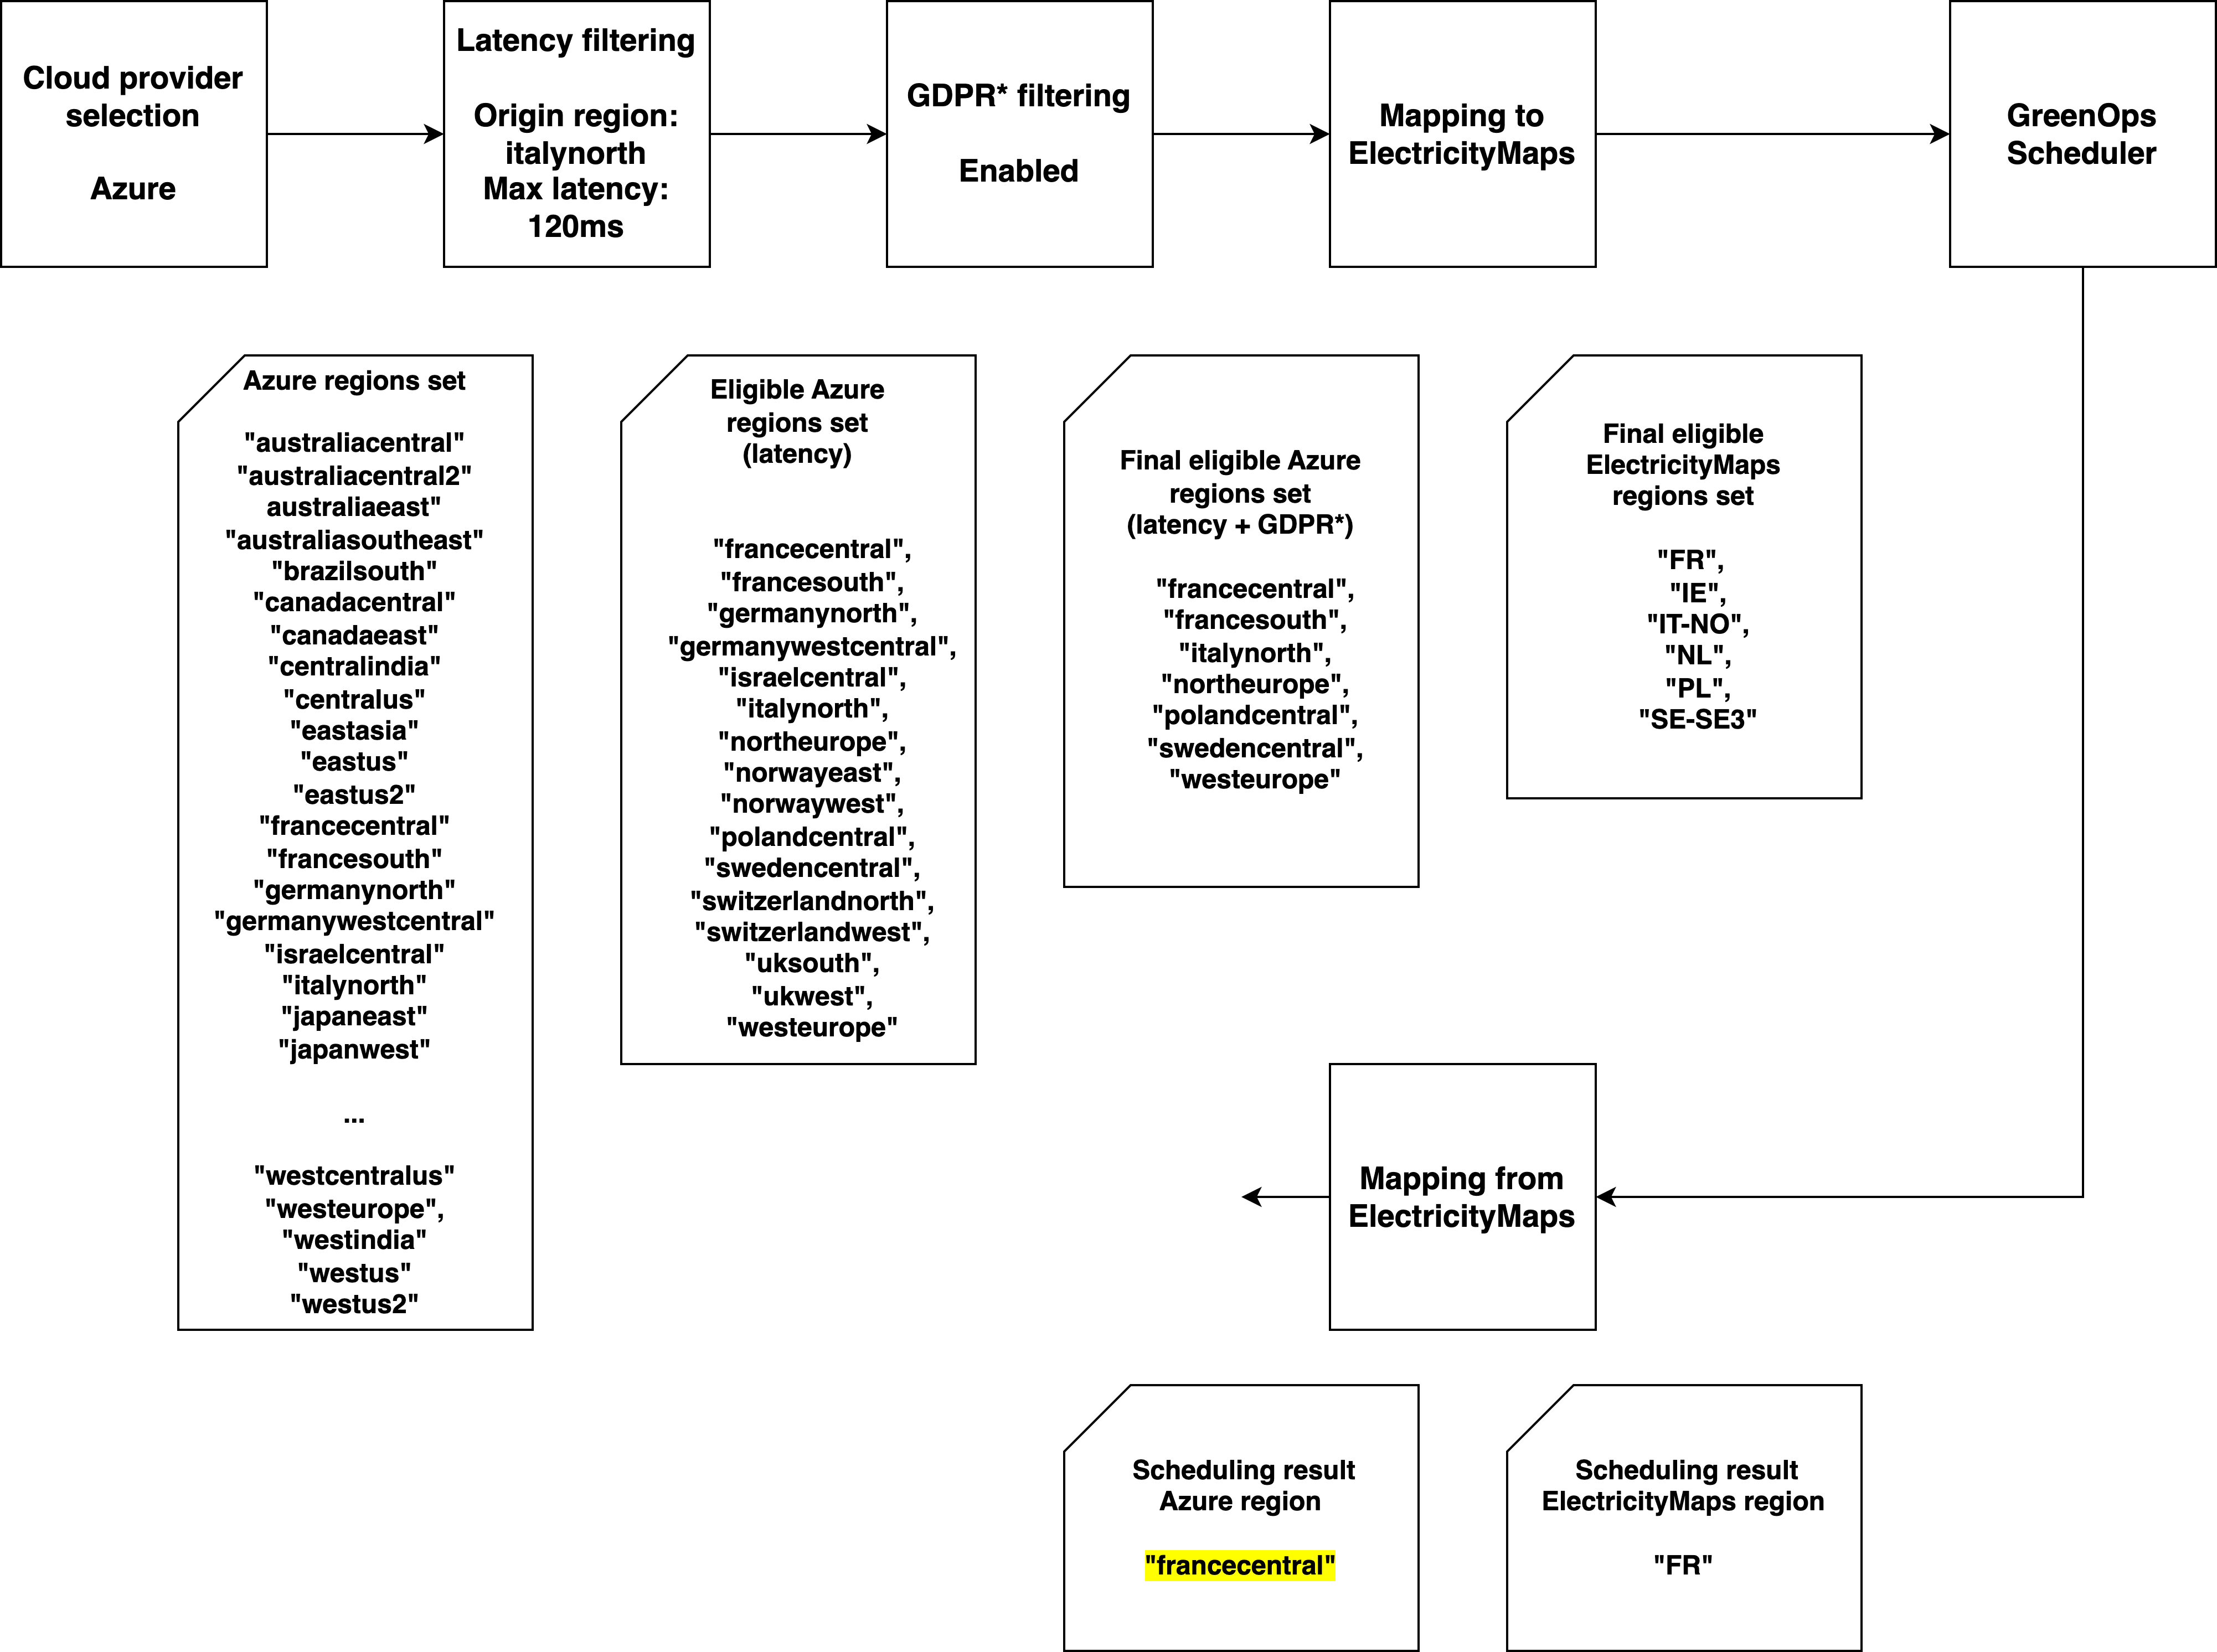
\includegraphics[width=1\linewidth]{images/data_mapping.png}
  \caption{OPA Data mapping}
  \label{fig:data_mapping}
\end{figure}

\begin{lstlisting}[language=Rego, caption=Rego data mapping, label=lst:rego_data_mapping]
# Utility functions to map between cloud provider regions 
# and ElectricityMaps regions

map_to_electricitymaps(eligible_regions, provider) = em_regions if {
    em_regions := {
        region.ElectricityMapsName |                             
        some eligible_region;                       
        some region;                                
        eligible_region = eligible_regions[_];      
        region = data[provider].cloud_regions[_];   
        region.Name == eligible_region             
        region.ElectricityMapsName != ""            
        region.ElectricityMapsName != "Unknown"
    }
}

map_from_electricitymaps(em_region, provider) = cloud_region if {
    some region;                              
    region = data[provider].cloud_regions[_];   
    region.ElectricityMapsName == em_region;    
    cloud_region := region.Name 
}

\end{lstlisting}

\subsection{OPA integration in the system}

In this section we describe the integration of OPA in the system.
The entire architecture of the system and the integration of OPA is illustrated in figure \ref{fig:architecture}.
OPA has the role of \textbf{mutating webhook server} which is consulted by the Kubernetes API server when a CREATE or UPDATE operation is performed on a VmTemplate Custom Resource.
The OPA server is responsible for evaluating the policies and returning the AdmissionReview response to the API server.
The AdmissionReview response contains the decision of the policy evaluation (i.e. scheduling outcome) and the JSON patch operations to be applied to the VmTemplate resource by the Kubernetes API server.
OPA is periodically polling the policy bundles from an external container registry (e.g., DockerHub) to ensure that the policies are up to date.
The main policy, namely the ``scheduling outcome policy'', is responsible for determining the scheduling decision based on the output of the GreenOps Scheduler called in real-time at request time, as described in section \ref{sec:scheduling_outcome_policy}.
OPA is also responsible for data mapping operations between ElectricityMaps regions and cloud provider regions, as described in section \ref{sec:opa_data_mapping}.
The system is designed to be highly flexible and extensible, allowing for the addition of new policies and data mappings as needed.

\begin{figure}[htb]
\centering
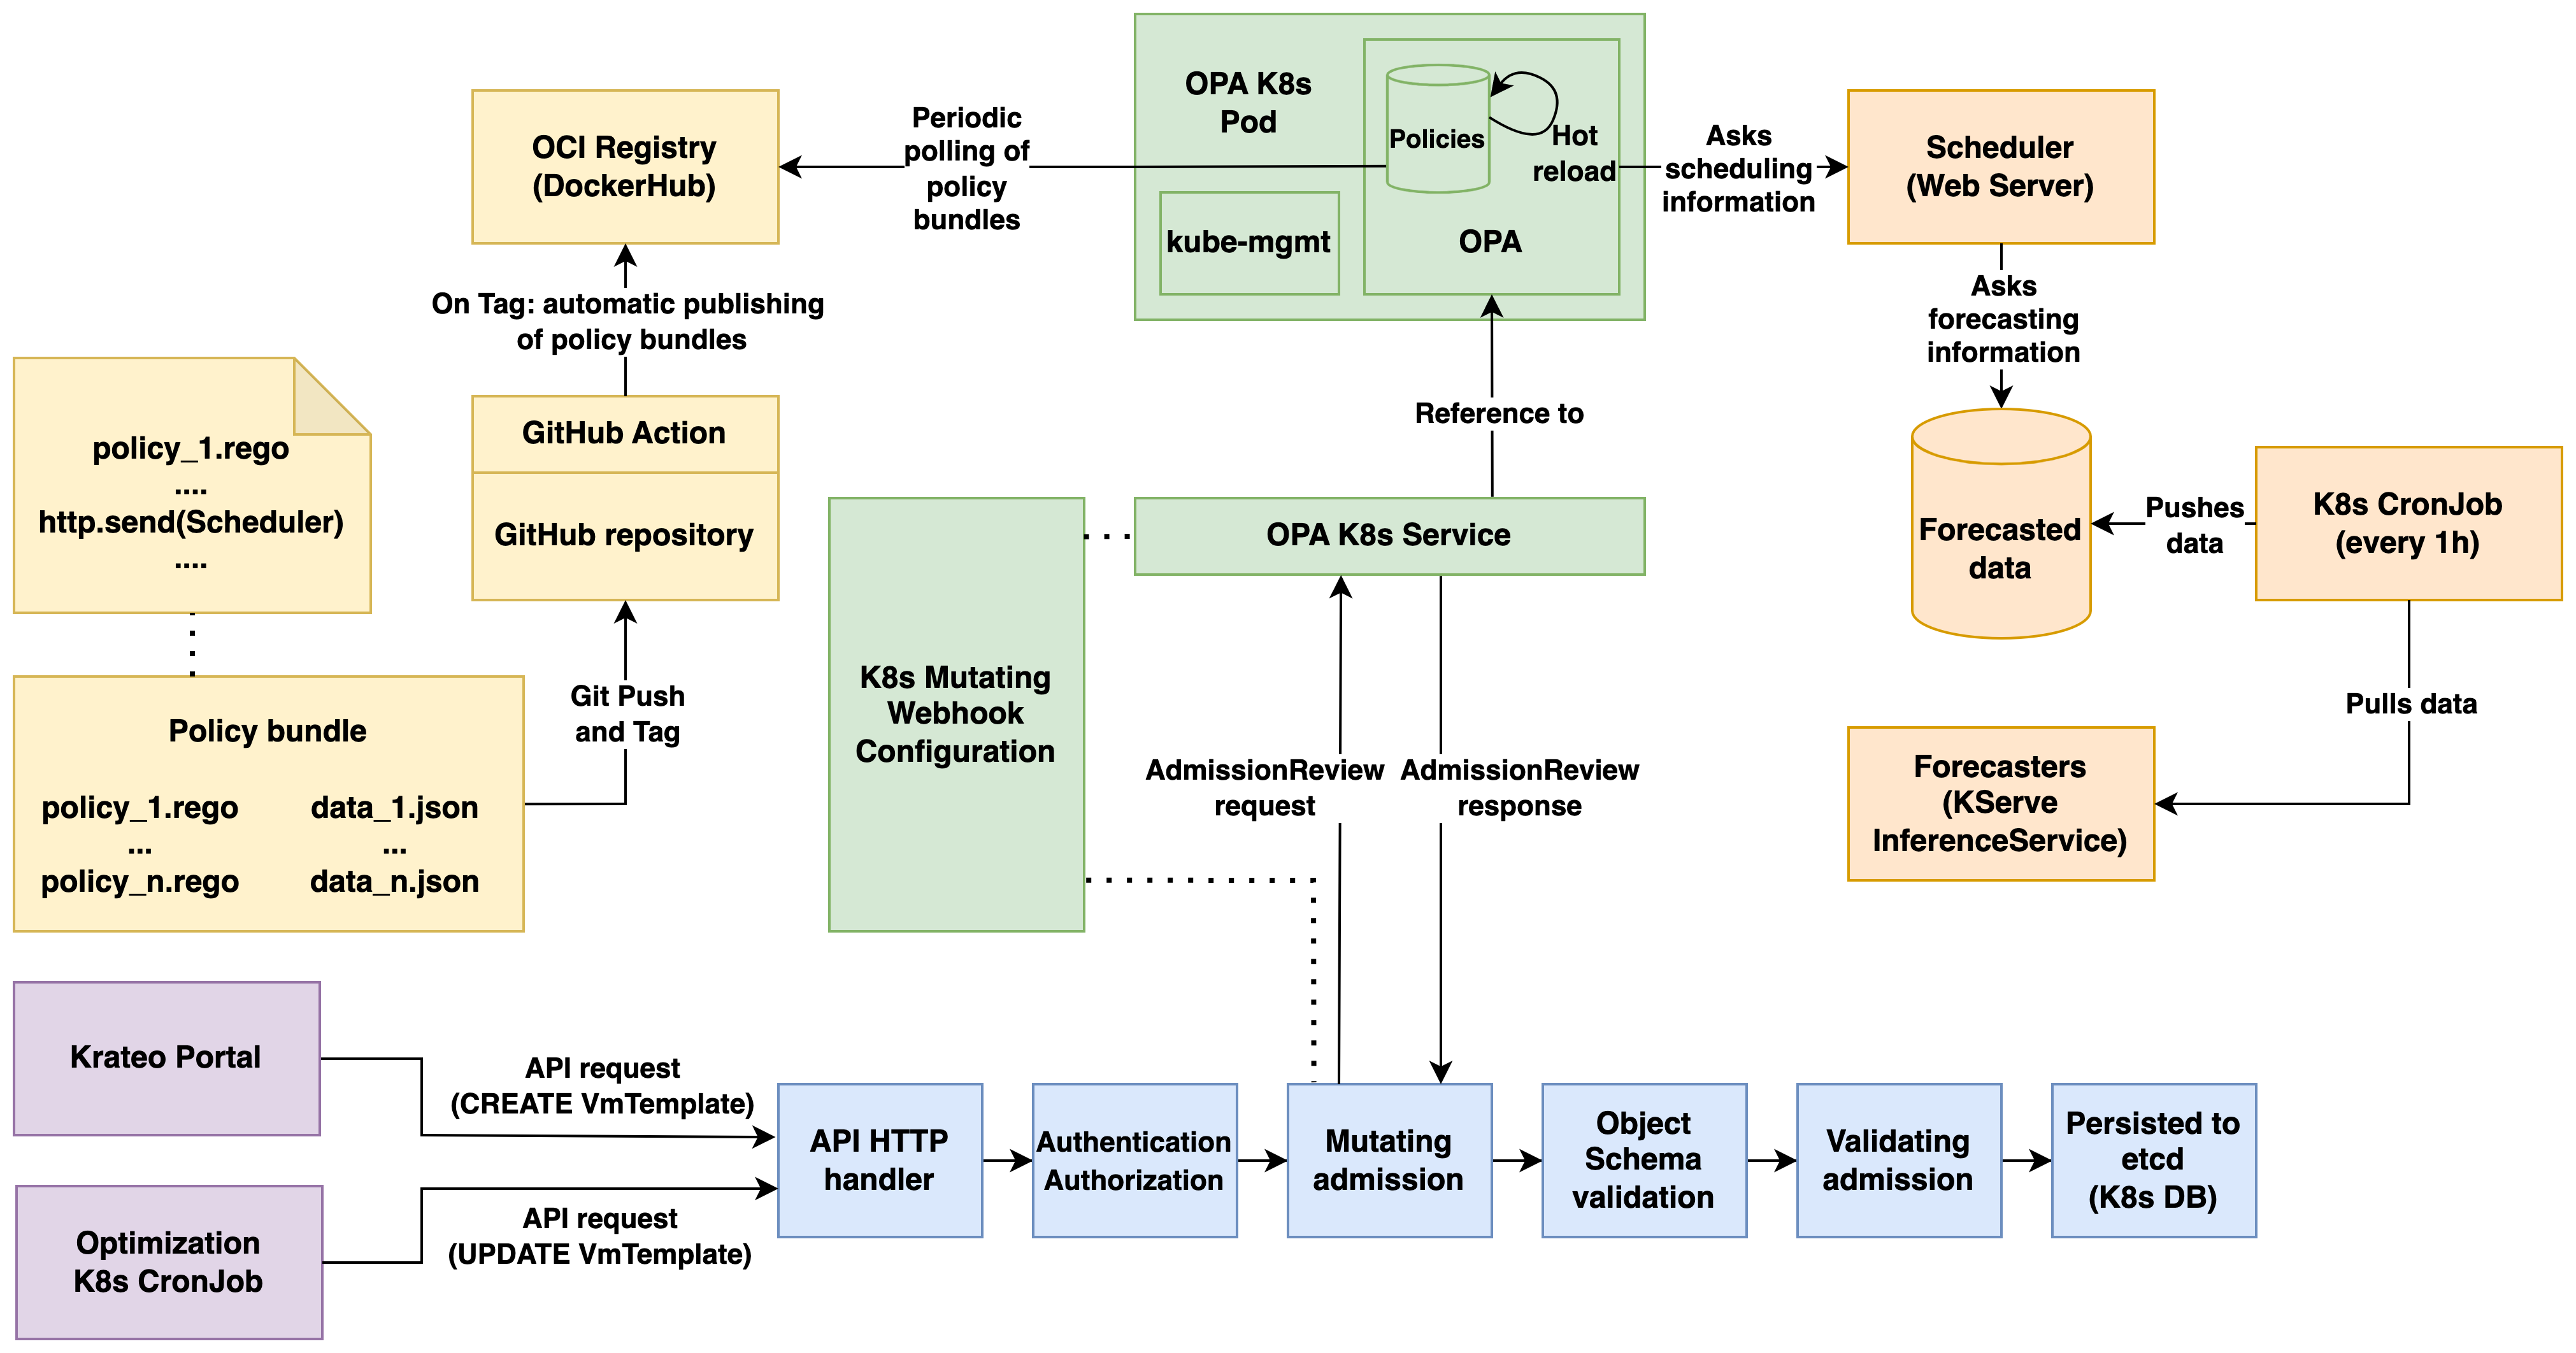
\includegraphics[width=1\linewidth]{images/architecture.png}
\caption{General architecture}
\label{fig:architecture}
\end{figure}

\subsubsection{Day 2 operations}
\label{sec:day2_operations}

We can define as \textbf{\textit{Day 2 operations}} all the management operations that are performed after the deployment of a resource.
These operations comprise tasks such as scaling up or down a VM based on the load, stopping a VM during off-peak hours, or migrating a VM to a different region to optimize costs.
As we previously described, the mutating webhook configuration is set on both the CREATE and \textbf{UPDATE} operations.
A possible UPDATE operation trigger could be Kubernetes Cronjob that attach a label \textit{"greenops-optimization": "123456789"} to the VmTemplate resource at a specific time of the day.
This could be useful to trigger specific policies that are only applied during the day 2 operations.
In addition to that, the UPDATE operation could be useful for VMs that have already been scheduled in a distant future (due to their deadline very far in the future) to obtain a new scheduling decision based on new conditions (e.g. more recent carbon intensity forecast).

\subsection{OPA Gatekeeper}

OPA Gatekeeper is a Kubernetes-native policy engine that extends OPA with \textbf{Custom Resources (CRs)} and controllers to enforce policies across a Kubernetes cluster \cite{opa_gatekeeper}. 
It integrates natively with Kubernetes and provides a declarative approach to defining and enforcing policies using Kubernetes Custom Resources (CRs). 
This makes it an excellent choice for basic and standard policy enforcement scenarios, such as RBAC (Role-Based Access Control), security compliance, and resource constraints \cite{opa_gatekeeper}.
However, while OPA Gatekeeper is \textbf{well-suited for simple use cases}, it presents \textbf{limitations} when addressing complex policy requirements, particularly when policies involve \textbf{mutations} or require access to \textbf{external data sources} \cite{opa_gatekeeper_external_data}. 
Indeed, these limitations make it unsuitable for the specific challenges tackled in this system. 
Therefore, after an initial investigation and Proof of Concept implementation, we decided to use a standard OPA server deployment for policy enforcement mainly due to the flexibility it provides in handling diverse scenarios.
To illustrate the differences between a standard OPA policy and an OPA Gatekeeper policy, we present two examples:  
\begin{itemize}[itemsep=0.2pt, topsep=1pt]
  \item[$\bullet$] a simple Rego policy that enforces a basic constraint on Pod creation in a Kubernetes cluster.
  \item[$\bullet$] the corresponding policy implemented as an OPA Gatekeeper \textbf{ConstraintTemplate} and \textbf{Constraint} Kubernetes custom resources.
\end{itemize}

The first example demonstrates a standalone Rego policy, which can be evaluated directly by an OPA instance. 
While this approach is flexible and allows for fine-grained policy definition, it requires manual integration into the system, including policy distribution and enforcement setup.  

\begin{lstlisting}[language=rego, caption={Simple OPA Rego Policy}, label={lst:opa-rego}]
package kubernetes.admission

deny[msg] {
  input.request.kind.kind == "Pod"
  input.request.object.metadata.namespace == "restricted"
  msg := "Pods cannot be created in the 'restricted' namespace."
}
\end{lstlisting}

The second example, illustrated in listing \ref{lst:gatekeeper-template} utilizes OPA Gatekeeper, which extends Kubernetes with Kubernetes-native Custom Resource Definitions (CRDs), enabling declarative policy management. By using a ConstraintTemplate, policies can be enforced dynamically through Kubernetes, making them easier to distribute and manage.
In other words, with this kind of setting, OPA policy bundles are not employed in the same way as in the standard OPA server. Instead, policies are defined as Kubernetes resources, allowing for more straightforward policy enforcement and management within a Kubernetes environment.

\begin{lstlisting}[language=yaml, caption={OPA Gatekeeper ConstraintTemplate}, label={lst:gatekeeper-template}]
apiVersion: templates.gatekeeper.sh/v1
kind: ConstraintTemplate
metadata:
  name: podnamespaceconstraint
spec:
  crd:
    spec:
      names:
        kind: PodNamespaceConstraint
  targets:
    - target: admission.k8s.gatekeeper.sh
      rego: |
        package kubernetes.admission
        deny[msg] {
          input.review.object.metadata.namespace == "restricted"
          msg := "Pods cannot be created in the 'restricted' namespace."
        }
\end{lstlisting}

\begin{lstlisting}[language=yaml, caption={OPA Gatekeeper Constraint}, label={lst:gatekeeper-constraint}, float=htpb]
apiVersion: constraints.gatekeeper.sh/v1beta1
kind: PodNamespaceConstraint
metadata:
  name: restrict-namespace
spec:
  match:
    kinds:
      - apiGroups: [""]
        kinds: ["Pod"]
  parameters: {}
\end{lstlisting}

In the example, the policy is defined as a ConstraintTemplate, which is then instantiated as a Constraint Custom Resource of kind defined in the ConstraintTemplate. 
The ConstraintTemplate specifies the Rego policy logic, while the Constraint defines the target resources and parameters for policy enforcement. Therefore a ConstraintTemplate can be used by multiple Constraints, allowing for policy reuse.

OPA Gatekeeper also provides additional Kubernetes Custom Resources called \textit{mutators} (Assign, AssignMetadata, AssignImage, ModifySet) that allow modifying resource fields without writing Rego code \cite{opa_gatekeeper}. 
These mutators are useful for simple transformations, such as setting default labels or annotations. However simultaneous mutation of multiple fields leveraging external data is not supported \cite{opa_gatekeeper_external_data}. 
This limitation, in the context of our system, determined the choice of the standard OPA server for policy enforcement. \newline

It must be noted that OPA Gatekeeper limitations could be potentially addressed in future releases, making it a more viable option for complex policy enforcement scenarios. 
However, for the current system requirements, the standard OPA server was deemed more suitable due to its flexibility.

\subsection{OPA advanced features}

It is deemed useful to mention some of the advanced features of OPA that were not employed in the first iteration of the system described in this thesis but could be potentially useful in future developments or in other contexts where OPA is used.
\newline
To ensure data integrity of policies (i.e., to prevent unauthorized modifications or MITM (Man in the Middle) attacks) and to provide a mechanism for verifying the authenticity of policies, OPA provides a \textbf{policy signing} feature \cite{opa_signing}.
This feature allow policy developer to digitally sign their policies bundles by adding a file named ``\textit{.signature.json}''.
\newline
OPA also provides a more efficient way to distribute policies using \textbf{Delta Bundles} \cite{opa_delta_bundles}.
Normally, when a policy bundle is downloaded, OPA will download the entire bundle, erase and overwrite the current policies and data with the new ones.
Delta Bundles are composed of a single ``patch.json'' file that contains a set of JSON Patch operations that can be applied to the current data to update it to the new version. Currently only data updates are supported (``data.json") and not policy updates (``policy.rego") \cite{opa_delta_bundles}.

\newpage

\section{MLOps infrastructure}

MLOps is the abbreviation of ``\textbf{Machine Learning Operations}", and it broadly refers to a set of methods designed to improve workflow procedures and automate machine learning deployments. 
It enables the reliable and efficient management, maintenance and deployment of models at scale \cite{mlops_ubuntu}.
A MLOps infrastructure is not necessarily required for multi-cloud resource management, but it is believed that AI models will be utilized in the future more and more to get \textbf{scheduling and management decisions}, as evidenced by recent studies discussed in section \ref{sec:ai_based_resource_management}.
It is therefore deemed important to describe the MLOps infrastructure deployed in a Kubernetes environment and leveraged by the system described in this thesis.

\subsection{MLOps purpose}

In a way, MLOps implements DevOps principles, tools and practices into typical Machine Learning workflows.
Its main purpose is to effectively industrialize the machine learning models lifecycle, enabling faster model development, selection, and deployment to production compared to traditional manual approaches.
Some principles of MLOps can be summarized as follows \cite{mlops_ubuntu}:
\begin{itemize}[itemsep=0.2pt, topsep=1pt]
  \item[$\bullet$] \textbf{Automation}: automate the entire model lifecycle, from training to deployment.
  \item[$\bullet$] \textbf{Versioning}: track and version models (with related data and code).
  \item[$\bullet$] \textbf{Reproducibility}: ensure that various model versions can be reproduced at any time.
  \item[$\bullet$] \textbf{Monitoring}: monitor models in production to ensure they are performing as expected.
  \item[$\bullet$] \textbf{Scalability}: scale models to handle increased workloads in a seamless manner.
  \item[$\bullet$] \textbf{Collaboration}: enable collaboration between data scientists, data engineers, and operations teams.
\end{itemize}

In the context of the proposed system, an MLOps infrastructure is used to deploy and manage the forecasting models that predict the carbon intensity of the electricity grid in different world regions.
In particular, \textbf{MLflow} is used for model tracking, model selection, and model storage, while \textbf{KServe} is used for model deployment.

\subsection{MLflow}

MLflow is an open-source platform designed to facilitate and enhance the overall machine learning lifecycle. 
In particular, it offers tooling for \textbf{experiment tracking}, \textbf{model management}, and \textbf{model storage} \cite{mlflow_docs}.
It is compatible with various ML frameworks, including scikit-learn, PyTorch, TensorFlow, and XGBoost.
In particular, in the case of our system, PyTorch is the ML framework used for the forecasting models making MLflow a suitable choice for model management.
For what concerns model deployment, MLflow does not provide a built-in solution, but it is compatible with other tools like KServe which will be described in section \ref{sec:kserve}.

\subsubsection{MLflow Tracking Server}
\label{sec:mlflow_tracking_server}

MLflow Tracking Server is the central component of the MLflow platform which is responsible for logging and storing model training data, parameters, and metrics. 
It enables ML practitioners to track experiments, compare results, and reproduce models easily in a collaborative environment.
MLflow Tracking Server revolves around the concepts of \textbf{experiments}, which are collections of \textbf{runs}. 
Each run represents a single model training session, and it contains information such as parameters, metrics, and artifacts (e.g., model files).
Selected models can then be registered in the MLflow Model Registry, which is essentially an optional subset of the selected models that are ready for deployment.
Model selection can done with the aid of a user interface that allows ML practitioners to visualize and compare the results of different experiments, making it easier to select the best model for deployment.
MLflow Tracking Server, as the name suggest, is a server that is constantly waiting for new data to be logged. 
Said data comes from the various training scripts that are executed by the data scientists or machine learning engineers which are run in  training environments.
In particular the training scripts must be instrumented with the \textbf{MLflow API calls} to log the data in the remote MLflow Tracking Server.
This setting is very flexible since the training scripts can be run in any environment (e.g., local environment, Universities' HPC clusters), as long as they have access to the MLflow Tracking Server.
It is deemed important to mention some of the MLflow API calls that are used in the training scripts: the \textit{infer\_signature} and \textit{autolog} functions \cite{mlflow_docs}.
The \textit{infer\_signature} function captures the \textbf{input and output schema of the model}, which is important for the deployment of the model.
The \textit{autolog} function is used to automatically log the parameters and metrics of the model training session, without the need to manually log them. In particular, each supported ML framework has its own autolog function which is used to automatically log the parameters and metrics of the model training session.
The final phase of a model training session is the automatic creation of a \textbf{self-contained directory}, named after the experiment and run IDs, that contains all the necessary files to deploy the model. 
In particular, the folder contains: the serialized model with model weights, the configuration files (conda.yaml, requirements.txt), and the MLmodel file that contains additional configuration, among which, the model signature.
The self-contained folder is then automatically uploaded to the MLflow Tracking Server as an artifact.
The following is an example of the structure of the self-contained directory created by MLflow after a PyTorch model training session: \\

\dirtree{%
.1 model/.
.2 MLmodel.
.2 conda.yaml.
.2 python\_env.yaml.
.2 requirements.txt.
.2 data/.
.3 model.pth.
.3 pickle\_module\_info.txt.
}

\subsubsection{MLflow deployment configuration}

In the context of our system, MLflow is deployed on a Kubernetes cluster with a loosely coupled architecture as can be seen in Figure \ref{fig:mlflow_config}, where the MLflow Tracking Server is decoupled from its storage: the metadata store (backend store) and the artifact store.
This configuration is the most common in production environments, as it allows for better scalability and environment flexibility.
The metadata store chosen for the system is \textbf{CrateDB}, while the artifact store is the \textbf{SeaweedFS} object storage service. \\

\begin{figure}[htb]
  \centering
  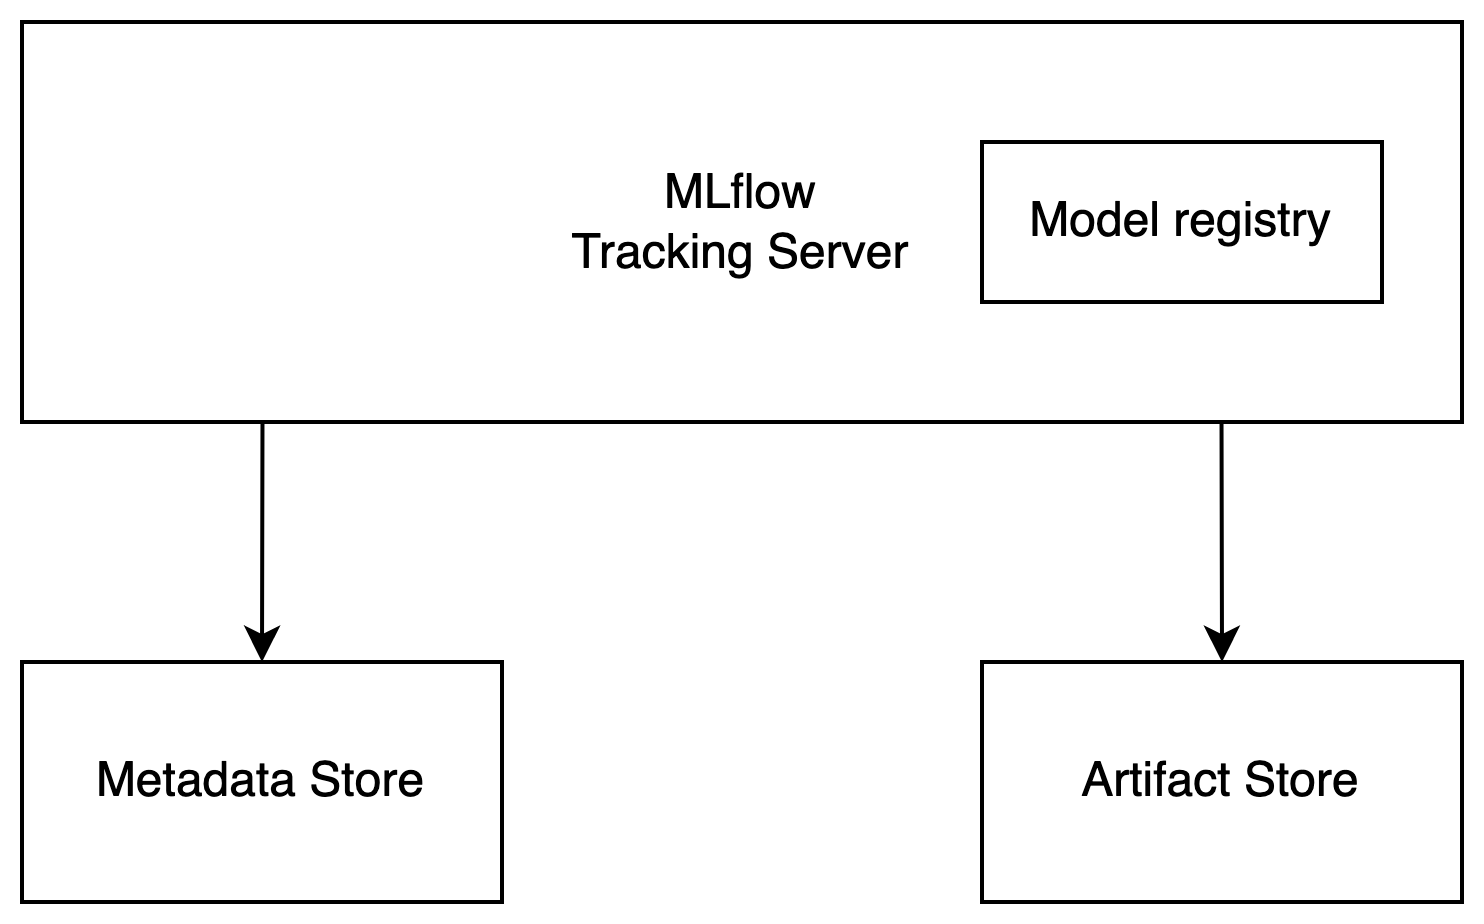
\includegraphics[width=0.50\linewidth]{images/mlflow_config.png}
  \caption{MLflow deployment configuration}
  \label{fig:mlflow_config}
\end{figure}

During the design phase, \textbf{alternative configurations} were considered.
One of the alternative configurations was to use a single CrateDB instance as both the metadata store and the artifact store. This configuration was not implemented due to the lack of native support of object storage in CrateDB.
A second theorized approach was to use a sidecar container with the duty of watching the MLflow Tracking Server local directory in the container filesystem (e.g., using \textit{watchdog} Python package), packaging the model artifacts as an OCI image, and uploading them to an image registry. This approach could be implemented to offer an alternative to the MLflow Tracking Server artifact store in environment where adding a new storage service is not feasible.

\subsection{KServe}
\label{sec:kserve}

KServe is an open-source model inference platform that extends Kubernetes with a set of Custom Resource Definitions (CRDs) to \textbf{deploy} and scale machine learning models in production environments \cite{kserve_docs}.
KServe can be deployed in several ways, one of which is the ``\textit{Serverless mode}'' which is built on top of Istio and Knative, leveraging their powerful capabilities such as automatic scaling. 
There are two main CRs that can be used to set up a model serving environment: \textit{\textbf{ServingRuntimes}} (or \textit{\textbf{ClusterServingRuntimes}}) and \textit{\textbf{InferenceServices}} \cite{krateo_docs}.
The former are abstractions that define model serving environments, specifying the templates for Kubernetes Pods capable of serving particular model formats. 
The latter are actually leveraging the available ServingRuntimes to deploy the models in the system.  
KServe provides several out-of-the-box ClusterServingRuntimes for common model formats, such as TensorFlow, PyTorch, and XGBoost, which can be used to deploy models without the need to define and configure the runtimes themselves.
In particular, in our specific use case, since the forecasting models are PyTorch models, packaged by MLflow as described in the previous section, InferenceServices with ``kserve-mlserver" ClusterServingRuntime are used. 
As a matter of fact, this runtime is the one that supports models packaged with MLflow \cite{kserve_mlflow}.
Listing \ref{lst:inference_service} shows an example of the InferenceService Custom Resource used to deploy a model in the system, namely the forectaser related to the ``\textit{IT-NO}'' ElectricityMaps region (northern Italy) \\

\begin{lstlisting}[language=yaml, caption={InferenceService Custom Resource example}, label={lst:inference_service}]
apiVersion: "serving.kserve.io/v1beta1"
kind: "InferenceService"
metadata:
  name: "forecaster-IT-NO"
  namespace: "model-inference"
spec:
  predictor:
    serviceAccountName: sa-s3creds
    model:
      modelFormat:
        name: mlflow
      protocolVersion: v2  
      storageUri: s3://mlartifacts/forecaster-IT-NO
\end{lstlisting}

We can see that the InferenceService CR is quite simple and self-explanatory. 
The most important fields are the \textit{model} field, which specifies the model format, the protocol version, and the storage URI.
The storage URI is the location of the model artifacts in the artifact store, which in the case of the system is the SeaweedFS object storage service with S3 compatibility. 
At the location specified by the storage URI, the model artifacts are stored in the self-contained directory created by MLflow after the model training session as described in section \ref{sec:mlflow_tracking_server}.

\subsubsection{Open Inference Protocol}

Interoperability is key in a fast-moving environment as the one of machine learning and AI. 
Therefore KServe has introduced the \textbf{Open Inference Protocol specification} to standardize the communication between inference servers and clients. 
The Open Inference Protocol has been adopted by several inference servers, including NVIDIA's Triton and Seldon MLserver \cite{kserve_oip}.
As mentioned in the previous section, the InferenceService CRs used in the system are leveraging the ``kserve-mlserver" ClusterServingRuntime, which under the hood uses MLserver that is compliant with the Open Inference Protocol.
The list of API endpoints specified by the Open Inference Protocol is shown in Table \ref{tab:oip_endpoints}.

% 

\begin{table}[h!]
\centering
\begin{tabular}{|l|l|l|}
\hline
\textbf{API}    & \textbf{Verb} & \textbf{Path}                                                                                         \\ \hline
Inference       & POST          & v2/models/{[}/versions/\textless{}model\_version\textgreater{}{]}/infer                               \\ \hline
Model Ready     & GET           & v2/models/\textless{}model\_name\textgreater{}{[}/versions/{]}/ready                                  \\ \hline
Model Metadata  & GET           & v2/models/\textless{}model\_name\textgreater{}{[}/versions/\textless{}model\_version\textgreater{}{]} \\ \hline
Server Ready    & GET           & v2/health/ready                                                                                       \\ \hline
Server Live     & GET           & v2/health/live                                                                                        \\ \hline
Server Metadata & GET           & v2                                                                                                    \\ \hline
\end{tabular}
\caption{Open Inference Protocol API endpoints specification \cite{kserve_oip}}
\label{tab:oip_endpoints}
\end{table}

\subsubsection{Model deployment}
\label{sec:model_deployment}

Our specific use case requires the deployment of multiple models, each corresponding to a different region.
This is true if we want to achieve better model performance compared to a single model that tries to predict the carbon intensity of all the regions.
The current strategy adopted for the system is the following: \textbf{one model per region} is deployed, and a \textbf{generic model is used as a fallback} if the specific model is not available.
This translates into the deployment of multiple InferenceServices, each corresponding to a specific region, and one InferenceService that acts as a fallback.
This setting introduces a quite large amount of overhead in terms of resources, since each InferenceService set up a whole new set of resources (e.g., large Kubernetes Pods with underlying model serving environments) for each model.
Figure \ref{fig:forecaster} illustrates the configuration of the InferenceServices used to deploy the forecasting models in the system.

\begin{figure}[htb]
  \centering
  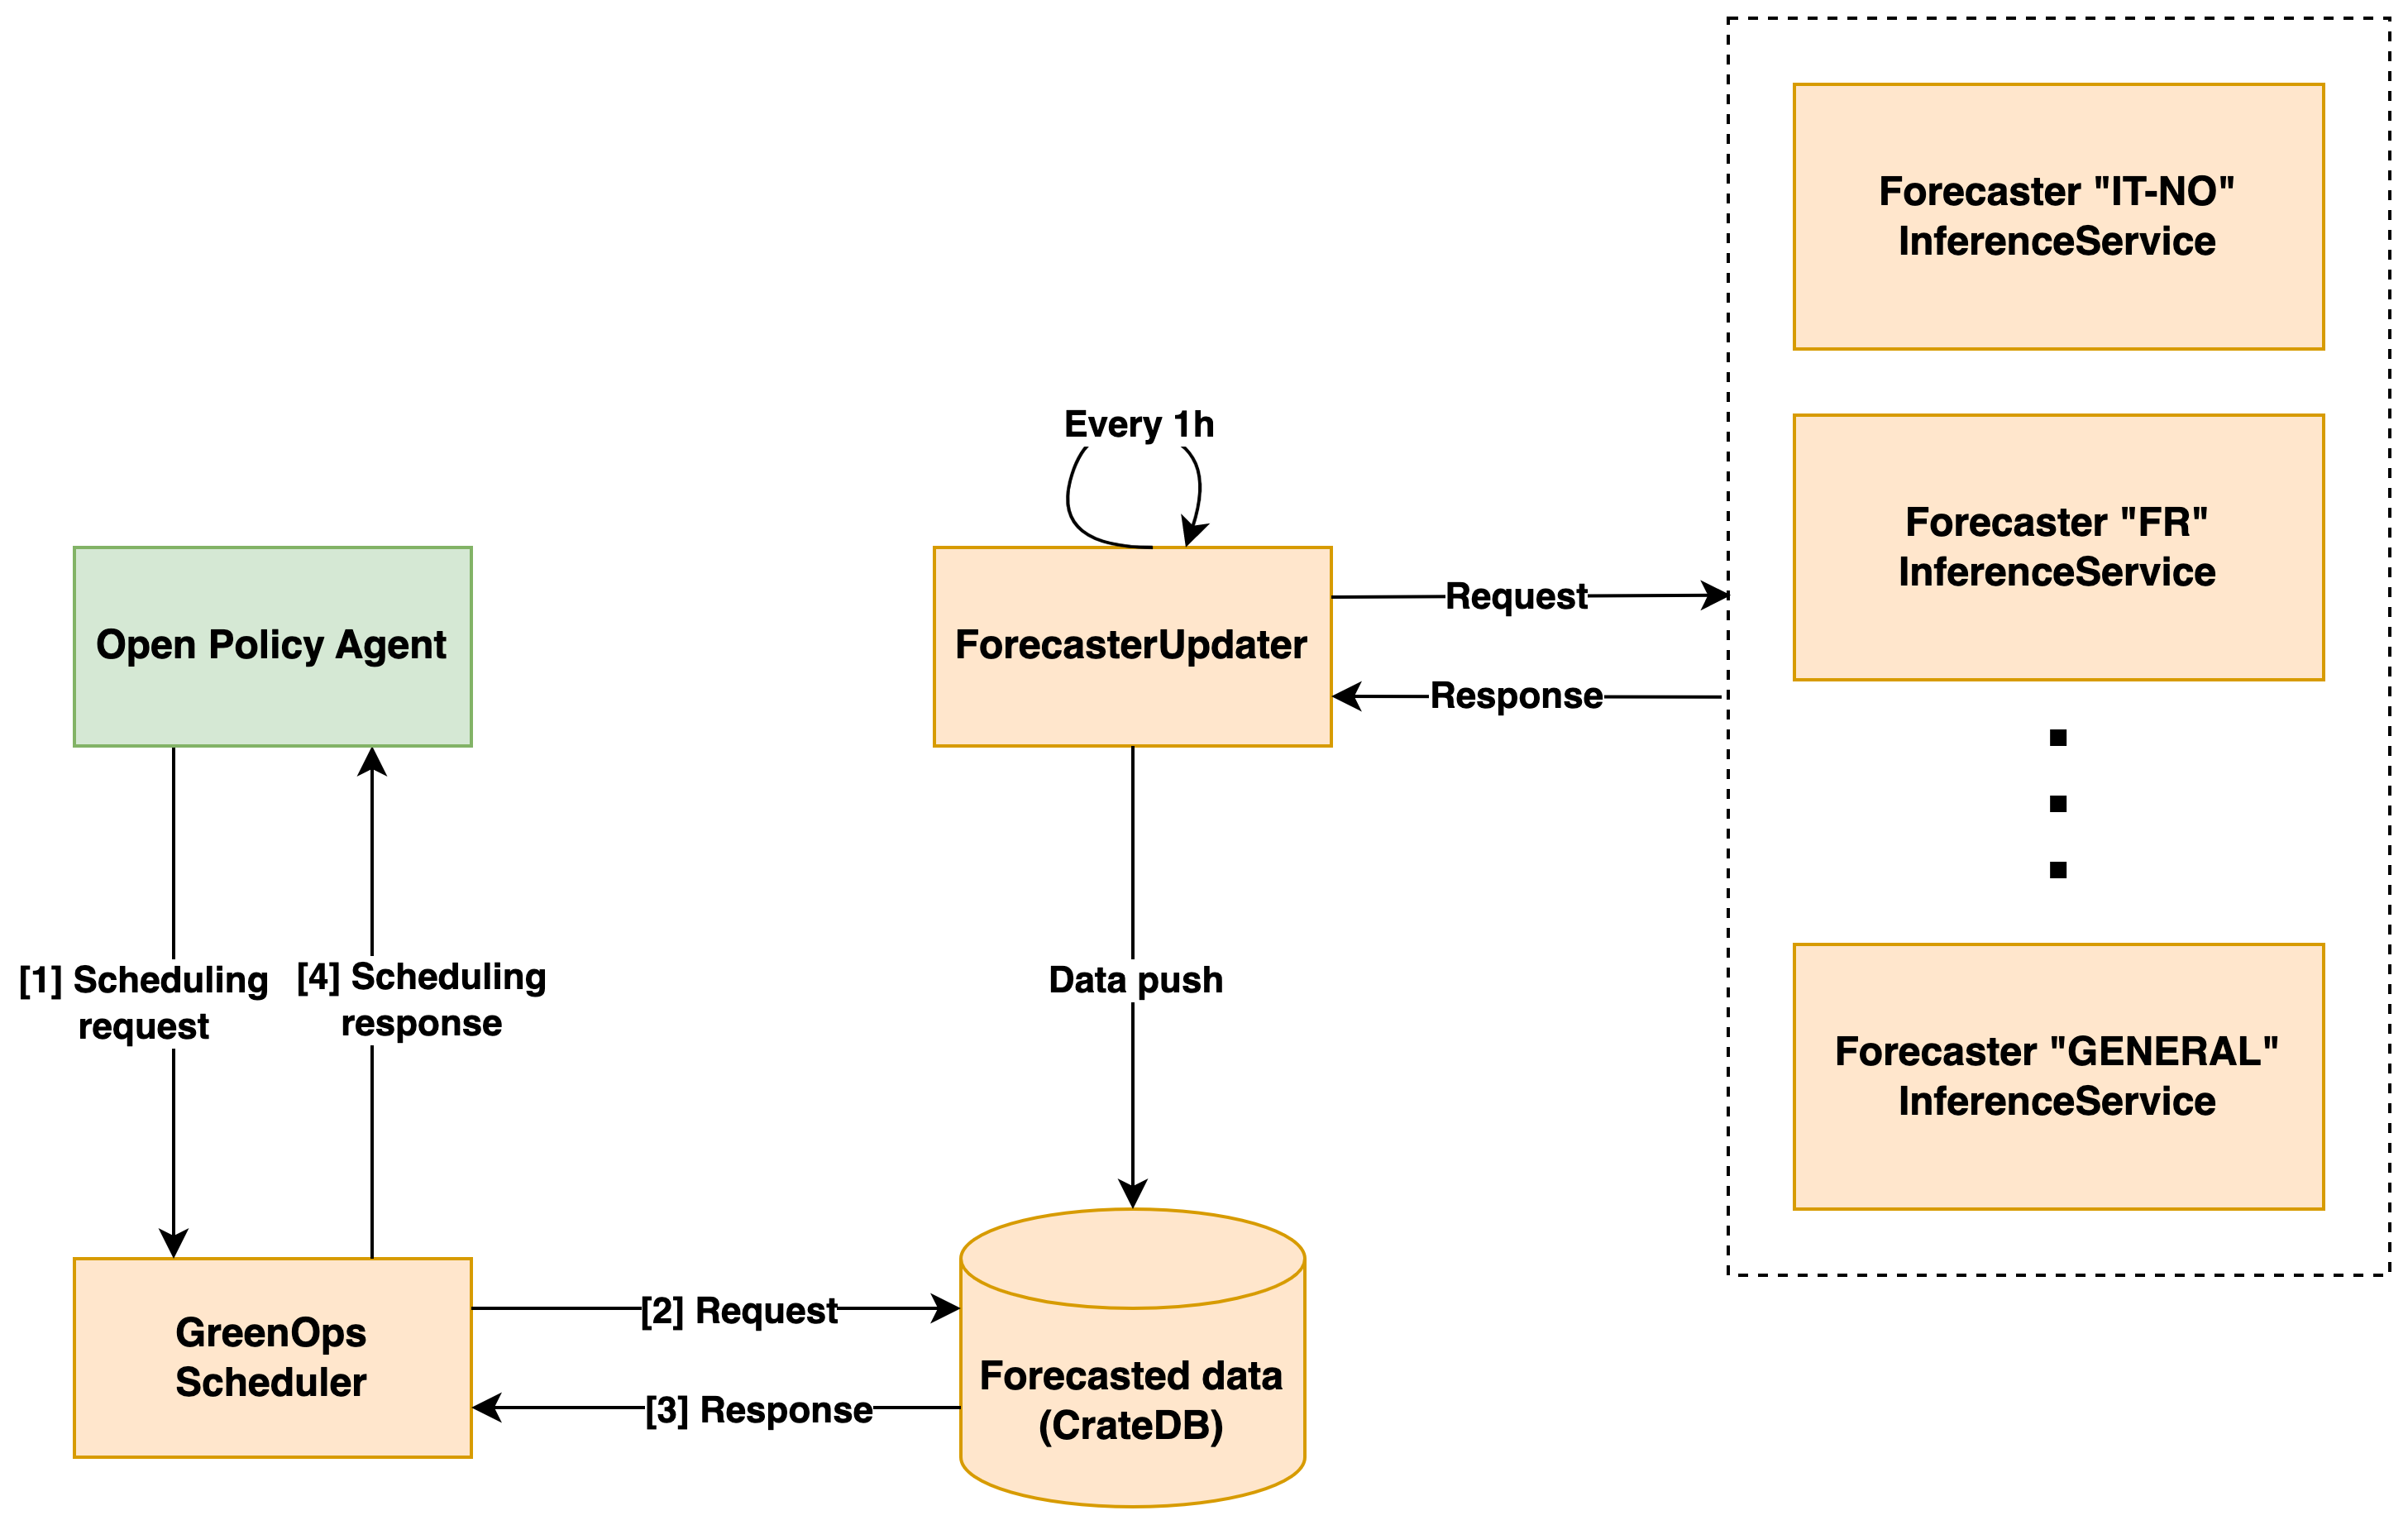
\includegraphics[width=1\linewidth]{images/forecaster.png}
  \caption{Model deployment configuration and GreenOps system integration}
  \label{fig:forecaster}
\end{figure}

\subsubsection{Model compatibility}

In scenarios where ML models produce outputs in formats not directly compatible with the serving runtime, some workarounds are necessary, such as model wrapping. This process involves adapting the model's input and output interfaces to align with the expected formats of the serving runtime, ensuring a correct model deployment.
For instance, in the case of the forecasting models, the output format was not directly compatible with the serving runtime: the output was a custom defined class specific to the model, instead of a single tensor. Therefore, a simple model wrapping was needed to make the model compatible with the serving runtime, effectively operation a selection of output fields from the model output and returning them as a single tensor.

\subsection{MLOps general architecture}

Figure \ref{fig:mlops} illustrates the general architecture of the MLOps infrastructure deployed in the Kubernetes environment. 
The architecture consists of two main components, described in the previous sections: MLflow and KServe.
In particular, MLflow is used for model tracking, model selection, and model storage, while KServe is leveraged for model deployment. 

\begin{figure}[H]
  \centering
  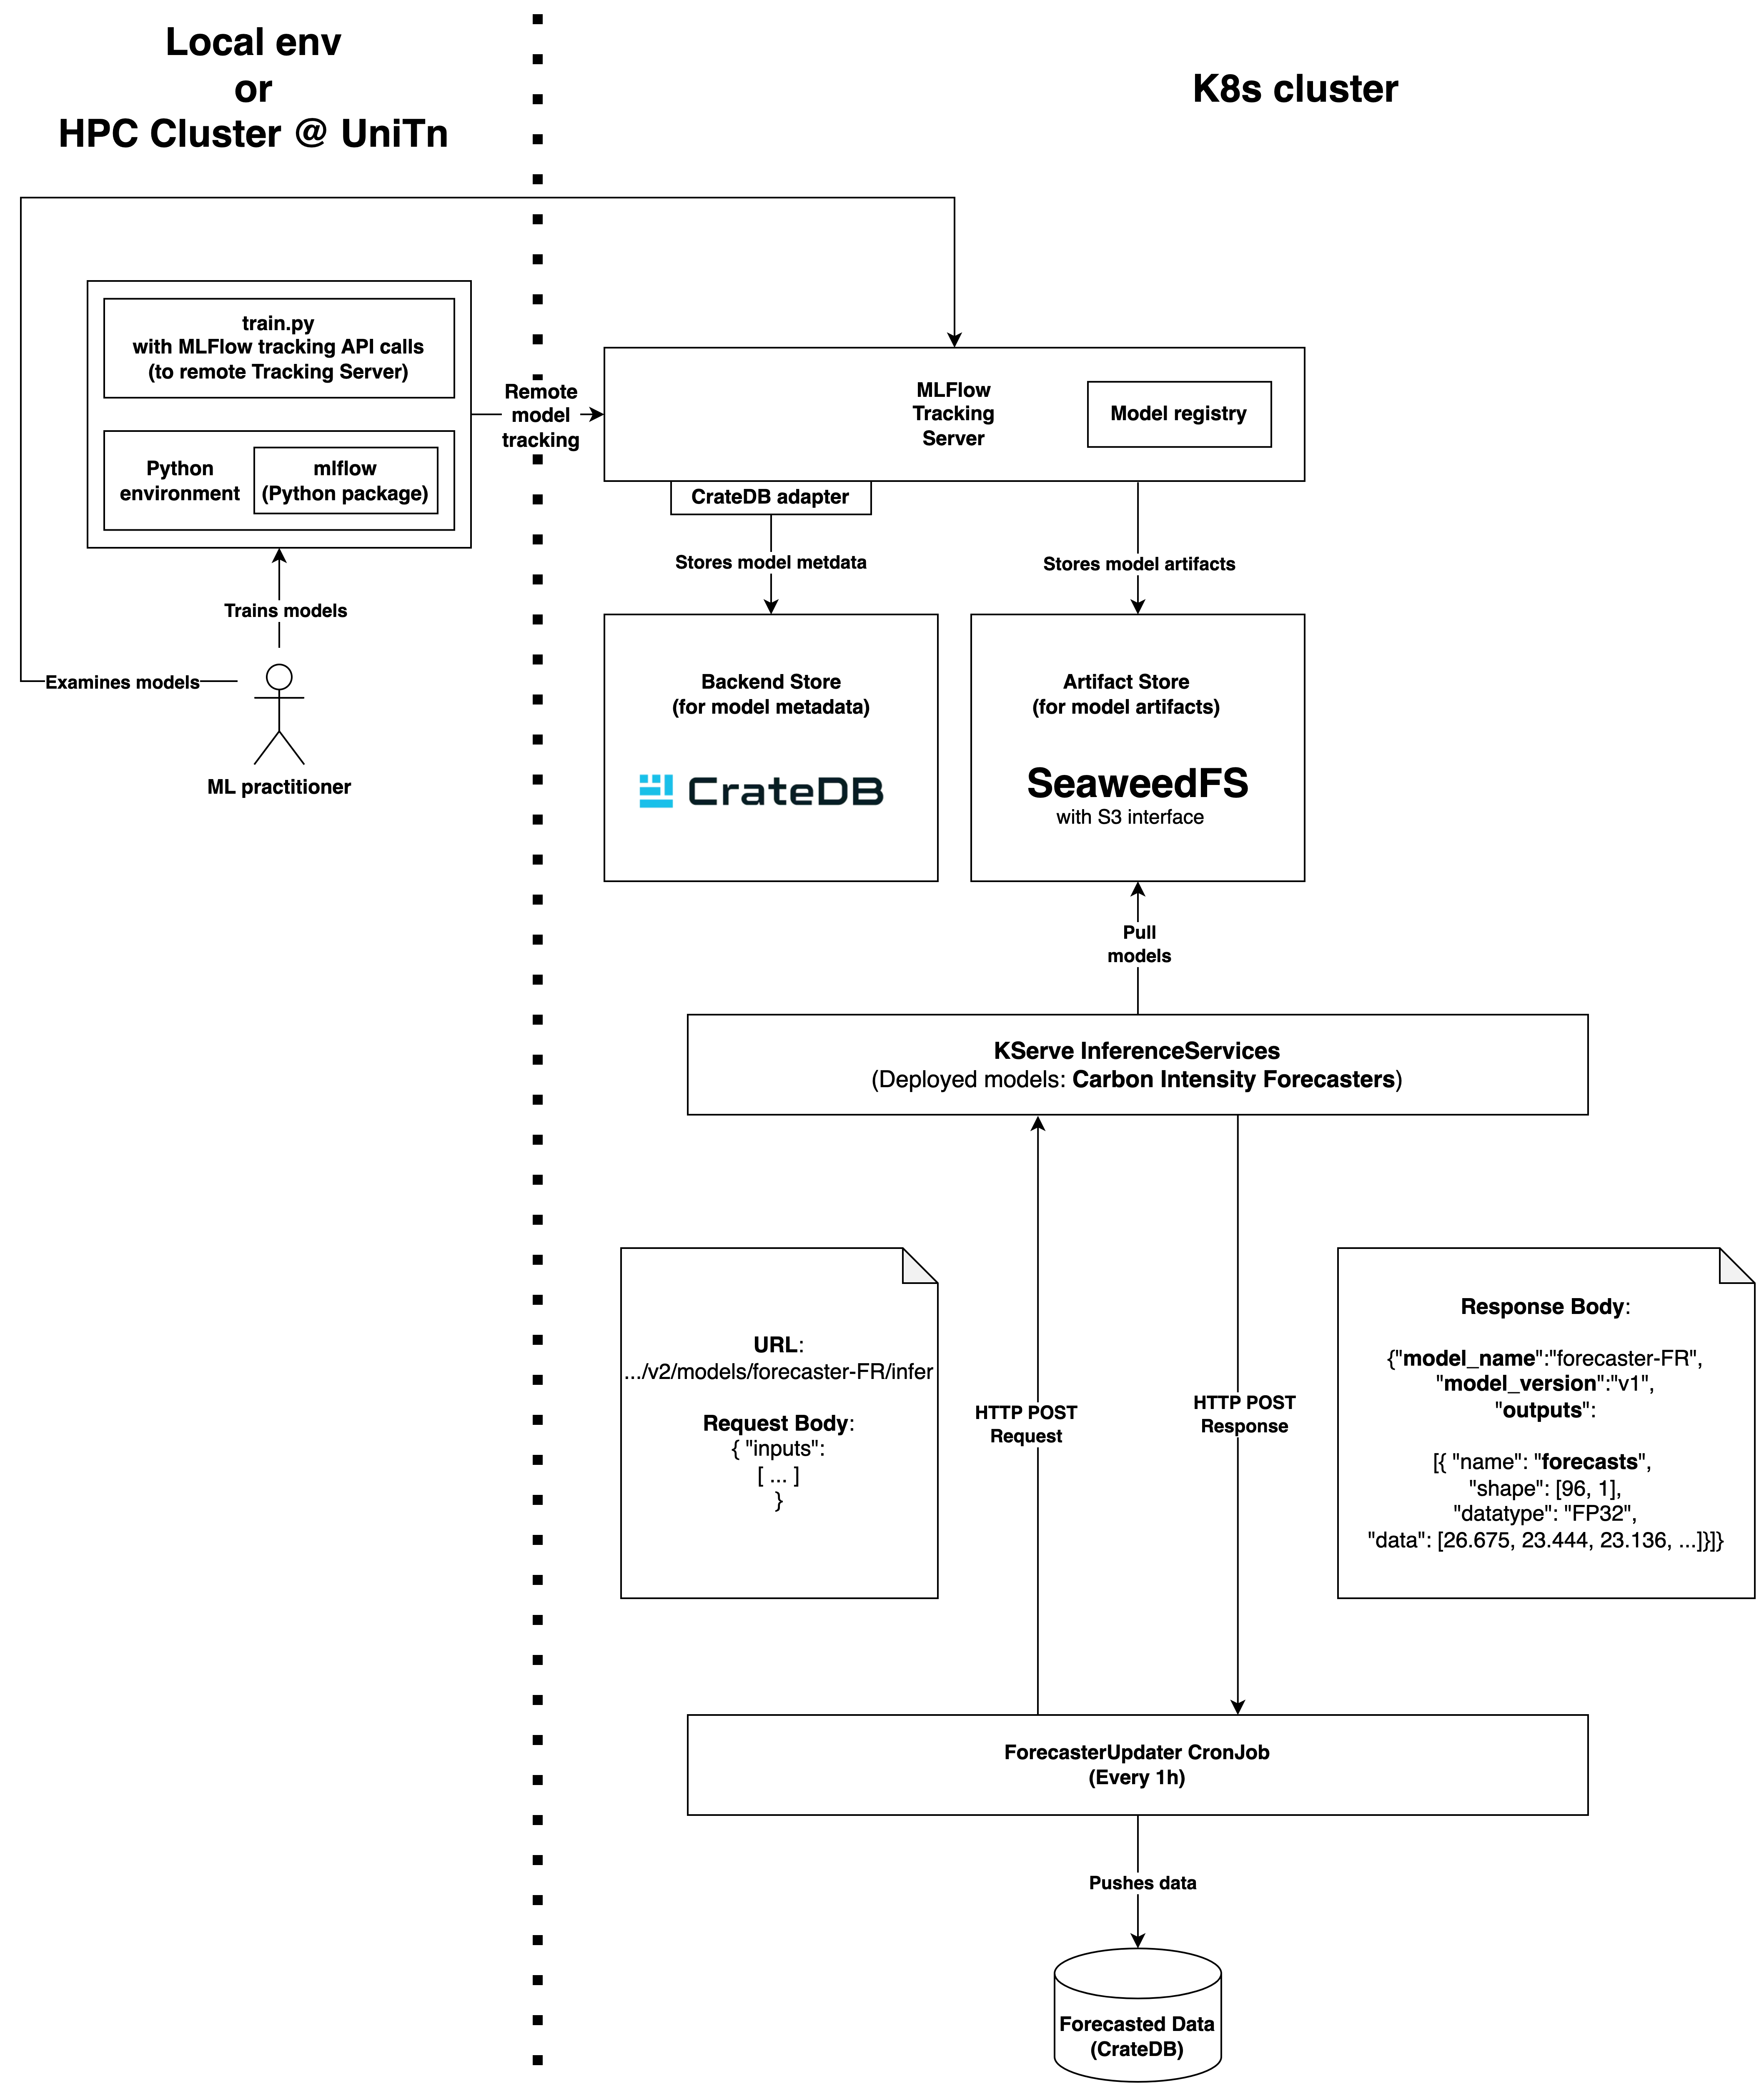
\includegraphics[width=1.00\linewidth]{images/mlflow_vertical.png}
  \caption{MLOps Architecture}
  \label{fig:mlops}
\end{figure}

\newpage

\section{Cloud resource metrics}

% https://dynamorio.org/google_workload_traces.html

Metrics are data points that provide information about a system.
This information could be related to performance, behavior, resource utilization or any other aspect of the system that could be relevant.
In the context of cloud resource management, metrics are essential for monitoring the \textbf{performance and health of cloud resources}, enabling organizations to make informed decisions about resource allocation, scaling, and optimization.
Focusing on the first use case of the proposed system (i.e., VM scheduling for carbon footprint optimization), carbon metrics could be used to determine the carbon footprint of a scheduled VM.
How to measure the carbon footprint of a resource managed in the cloud is a complex and challenging task.
The carbon footprint of a cloud resource is influenced by several factors, such as the energy efficiency of the data center where the resource is hosted (PUE), the carbon intensity of the electricity grid in the region where the data center is located, whether the data center uses additional energy sources off the grid, and finally the energy consumption of the resource itself.
The last factor is probably the most difficult to measure, as a cloud resource is an \textbf{entity that is abstracted from the physical infrastructure}, and therefore it is not straightforward to measure its power consumption. 
In this first iteration of the system we are dealing for instance with virtual machines (VMs).
On the other hand, an on-premises server, for instance, could be potentially equipped with physical sensors that measure the direct power consumption of the server, but this is not the case for any cloud resource, especially since this work is focused on the consumer side of the cloud, where the consumer does not have access to any physical infrastructure.
Moreover, public cloud providers do not provide fine grained and real-time data about the carbon footprint of a resource, as they do not adhere yet to a common standard for carbon footprint calculation (e.g., Real Time Cloud proposed by the Green Software Foundation), like they instead do for the FOCUS standard for FinOps.
In this section we want to give an brief overview of several metrics and methodologies that can be used totextbf{estimate the carbon footprint of a cloud resource}.
In addition, we will also discuss the \textbf{challenges and limitations} that can be encountered when dealing with this kind of task.

\subsection{System performance metrics}

System performance metrics are a category of metrics that provide information about the health and performance of a system.
Usually these metrics are related to bare-metal servers or virtual machines.
Other cloud resources that have a higher level of abstraction (e.g., containers, Kubernetes Pods, serverless functions) may expose a slighlty different set of metrics that fall into this category as well.
This category of metrics are also useful for the ``\textbf{day 2 operations}'', which are operations that are performed after the resource has been deployed and monitored for a certain period of time, briefly described in section \ref{sec:day2_operations}.

System performance metrics comprise, for instance:
\begin{itemize}[itemsep=0.2pt, topsep=1pt]
  \item[$\bullet$] CPU usage
  \item[$\bullet$] Memory usage
  \item[$\bullet$] Disk usage
  \item[$\bullet$] Network usage
  \item[$\bullet$] Processes related metrics \\
\end{itemize}

A standard strategy to collect these metrics is to use \textbf{agents} that are directly installed on the VMs and operate at the Operating System level.
Some examples of this kind of agents are the \textbf{Prometheus Node exporter} and the \textbf{Prometheus Process exporter}.
Figure \ref{fig:prometheus} shows an example of a standard Prometheus architecture used to collect system performance metrics using the Node exporter and the Process exporter on a set of Linux VMs.
In particular, the Node exporter collects metrics such as CPU usage, memory usage, disk usage, and network usage, while the Process exporter collects metrics about the various processes running on the VM (e.g., CPU and memory usage per process group).
Metrics are pulled by the Prometheus server, which stores them in a time-series database and makes them available for querying and visualization (e.g., using Grafana). 
In addition, the Prometheus server can be configured to send alerts based on the collected metrics leveraging the Alertmanager component. \newline

\begin{figure}[htb]
  \centering
  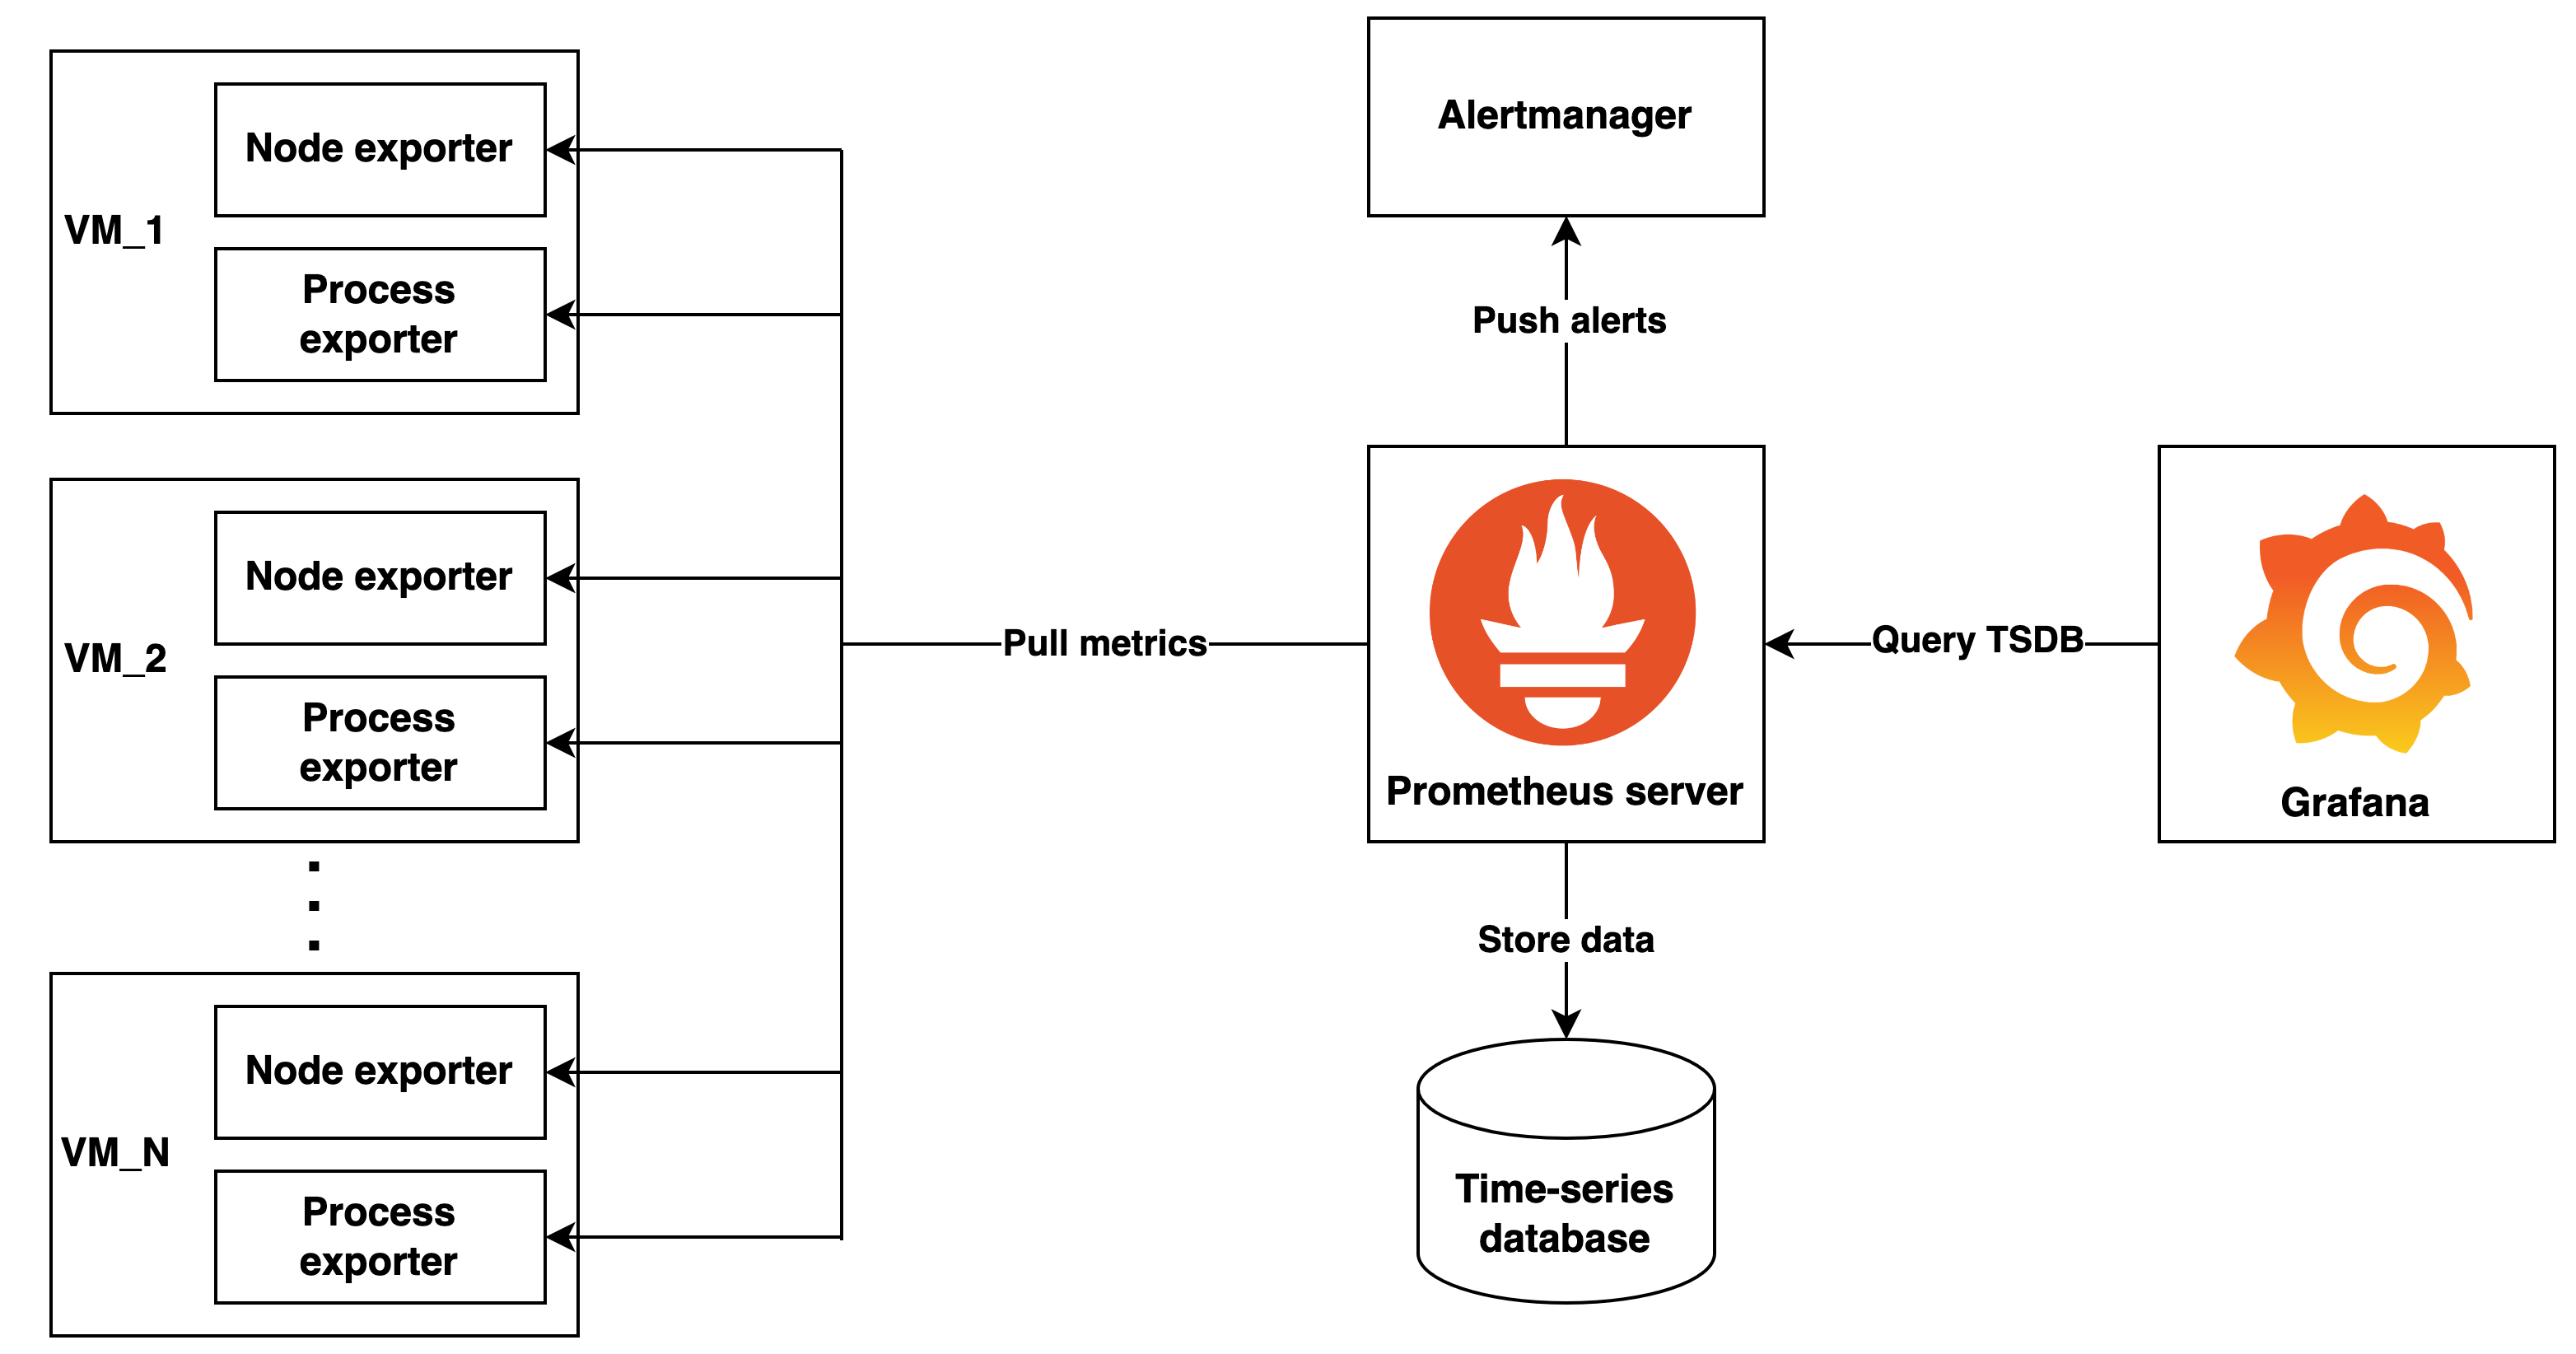
\includegraphics[width=1\linewidth]{images/prometheus.png}
  \caption{Standard Prometheus architecture for system performance metrics collection}
  \label{fig:prometheus}
\end{figure}

An example of how these metrics can be used for ``day 2 operations" is the one put in place by the \textbf{Krateo Composable FinOps} component \cite{krateo_docs}.
In this case, the system uses a set of Prometheus exporters and scrapers, configured through Kubernetes Custom Resources, to collect metrics about the VMs managed by the system.
The optimizations are encoded in a set of Kubernetes Custom Resources (CRs) that are used by the specific operators (e.g., \textit{finops-operator-vm-manager}) to performs operations on the VMs, such as scaling up or down the VMs, stopping them during off-peak hours, etc \cite{krateo_docs}.
%Prometheus exporters (https://prometheus.io/docs/instrumenting/exporters/) + Prometheus scrapers for data collection.
%Generic Prometheus exporters and scrapers already used for Krateo Composable FinOps leveraging specific K8s Custom Resources. These exporters are generic and can scrape arbitrary metrics configured in specific CRs (for instance, collecting VMs CPU consumption though Azure APIs).
%From the Krateo Composable FinOps document: 
%- “we transform all optimizations into a set of Kubernetes Custom Resources (CRs) to act upon newly found cost-related deficiencies. This allows us to use Kubernetes operators (explicitly coded to interact with cloud services) to monitor these metrics and act automatically to apply changes to remote resources.”
%- “forward the optimization to the Krateo operator that manages the services that need to be optimized, for example, the Azure Operator to modify the size of a Virtual Machine;”
%- “the optimization is automatically encoded in a CR for the finops-operator-vm-manager, which then analyzes it and decides how to manage the Virtual Machine. For example, it could scale up or down the virtual machine, stop it for the night, etc.”
\newline
As Microsoft Azure documentation describes, there are actually two different categories of metrics that can be collected from a VM in the cloud: the \textbf{guest-level metrics} and the \textbf{hypervisor-level or host-level metrics} \cite{azure_vm_monitoring}.
The first category of metrics is collected by agents directly installed on the VMs, as described above.
The second category of metrics is collected by \textbf{cloud provider APIs}, and they provide information about the VMs from the hypervisor or host level.
For instance, in the case of Azure Virtual Machines, this date is relaated to the Hyper-V host that runs the VM \cite{azure_vm_monitoring}.
The difference between these two categories of metrics is that the guest-level metrics are more fine-grained and provide information about the actual resource usage of the VM (being collected at the OS level), while the hypervisor-level metrics are more high-level. \newline
%Azure monitoring REST API: https://learn.microsoft.com/en-us/azure/azure-monitor/essentials/rest-api-walkthrough?tabs=rest%2Cportal
%https://learn.microsoft.com/en-us/rest/api/monitor/metrics/list?view=rest-monitor-2023-10-01&tabs=HTTP
%https://learn.microsoft.com/en-us/azure/virtual-machines/monitor-vm 
To support the collection of metrics, several cloud providers offer agents that can be installed on the provider-specific VMs they manage.
One of the goal of these agents comparared to standard cloud-agnostic agents is to provide a more convenient experience for the user managing the VMs in the context of the cloud provider. 
Therefore these agents are usually more integrated with other cloud provider services and APIs.
In particular, we can cite the following agents: \textbf{Azure Monitor Agent} for Azure VMs, the \textbf{Google Ops Agent} for Google Compute Engine instances, and the \textbf{Amazon CloudWatch Agent} for AWS EC2 instances.
%Azure Monitor Agent (https://learn.microsoft.com/en-us/azure/azure-monitor/agents/azure-monitor-agent-overview)
%\textbf{Google Ops Agent}: “the primary agent for collecting telemetry from your Compute Engine instances” (https://cloud.google.com/monitoring/agent/ops-agent)
%Can be installed in various ways: manual installation, Usining Google Cloud Agent policies from glcoud CLI or using a configuration management tool like Terraform

\subsection{Power consumption metrics}

In the context of our use case, power consumption metrcis could be theoretically used to estimate the carbon footprint of a VM instance.
However, Public Cloud Providers do not provide real-time data about power consumption of a VM instance. \\

\textbf{Scaphandre} is an open-source monitoring agent designed to collect energy consumption metrics of a system \cite{scaphandre}.
Scaphandre represents a promising solution only for on-premises servers, as it relies on the Intel \textbf{Running Average Power Limit (RAPL)} sensors to collect power consumption data.
As a matter of fact, due to security and privacy concerns, public cloud providers do not expose to tenants the underlying RAPL sensors that Scaphandre relies on to track energy consumption \cite{scaphandre_github_issue}.
Therefore, Scaphandre is unsuitable for our current use case.
Another interesting and quite mature project is \textbf{Kepler} \cite{kepler}, which is a tool designed to monitor the energy consumption of Kubernetes resources (e.g., Nodes, Pods).
Being Kubernetes-centric, Kepler is not suitable for our first use case, as it does not provide real-time data about the power consumption of a generic VM instance.
However, Kepler could be potentially used in a future iteration of the system.

%manually estimate power consumption based on CPU utilization, memory usage. Could be a very difficult task. 
%there is the TEADS metodology like 

\subsection{Carbon metrics}
\label{sec:carbon_metrics}

As briefly mentioned in the beginning of this section, there is no adopted standard adopted by Public Cloud Providers to calculate and expose the carbon footprint of a cloud resource.
In section \ref{sec:real_time_cloud}, we briefly described that the Green Software Foundation is working on a standard called \textbf{Real Time Cloud} that aims to provide a common standard for carbon footprint calculation.
The goal would be to have a \textbf{real-time carbon metric} to be used for optimization and this metric would be added to the set of metrics that are already provided by the cloud providers (e.g., CPU usage, memory usage).
However, this standard is not yet adopted by any major Public Cloud Provider which in turn provide only high-level monthly reports for carbon emission data.
A brief summary, as reported by one of the proposers of Real Time Cloud \cite{cloud_provider_sustainability_reports}, is shown in Table \ref{tab:cloud_carbon_emissions_reports}.

\begin{table}[H]
  \centering
  \renewcommand{\arraystretch}{1.2} % Increase row height for readability
  \setlength{\extrarowheight}{2pt} % Add extra space between rows
  \begin{tabularx}{\textwidth}{|X|X|X|X|X|X|}
  \hline
  \textbf{Cloud Provider}     & \textbf{Project name}                          & \textbf{Scope}            & \textbf{Geographical resolution} & \textbf{Carbon resolution} & \textbf{Time resolution} \\ \hline
  Amazon Web Services (AWS)   & AWS Customer Carbon Footprint Tool             & Account, EC2, S3, Other   & Continental                      & 0.001 Metric Tons of CO2e  & Monthly                  \\ \hline
  Microsoft Azure             & Azure Carbon Footprint API Schema              & Account, Service          & Country and region               & 0.001 Metric Tons of CO2e  & Monthly                  \\ \hline
  Google Cloud Platform (GCP) & Google Carbon Footprint BigQuery Export Schema & Account, Project, Service & Country, region and zone         & 0.1 Kilograms of CO2e      & Monthly                  \\ \hline
  \end{tabularx}
  \caption{Cloud provider sustainability reports}
  \label{tab:cloud_carbon_emissions_reports}
\end{table}
%Export Azure carbon optimization emissions data (Preview) (probably not fine-grained as we want)

We deem interesting to mention some of the existing projects that can be used to estimate the carbon footprint of a cloud resource.
\textbf{Cloud Carbon Footprint} \cite{cloud_carbon_footprint} is a tool that uses cloud provider billing (i.e., AWS Cost and Usage Reports with Amazon Athena, GCP Billing Export Table using BigQuery, Azure Consumption Management API) and resource usage metrics to provide an estimation of the carbon footprint of a cloud resource. For live grid carbon intensity an integration with Electricity Maps API is supported \cite{cloud_carbon_footprint}.
Another tool within the GreenOps ecosystem is the \textbf{Aether} calculation engine \cite{aether}
Currently only AWS and GCP are supported as it uses AWS CloudWatch and Google monitoring
There is not the possibility to use a real-time Grid Carbon Intensity Coefficient since carbon data is extrapolated from “governative” data reports \cite{aether}.
A different approach to estimate the carbon footprint of resource, in particualar a virtual machine is the one proposed by the \textbf{carbond} agent \cite{carbond:2023:hotcarbon}. 
This agent must be installed on the VM and aims to provide a real-time estimation of the carbon footprint of the VM via a file-system API \cite{carbond:2023:hotcarbon}.
It should be investigated further whether this agent could be use in cloud environments, since those settings, as described above, do not provide access to the underlying hardware sensors that are usually used by agents to estimate the power consumption of the VM

%Example of a manual approach (not scalable due to tech specs research): https://devblogs.microsoft.com/sustainable-software/how-can-i-calculate-co2eq-emissions-for-my-azure-vm/ 
%The critical point here is to get/calculate the energy consumed by a cloud instance, since there are a huge number of technical configurations to find, retrieve and use for calculations.

\subsection{Impact framework potential integration}
\label{sec:impact_framework_integration}

A potential integration with the Green Software Foundation's Impact Framework is envisioned for the system.
Currently, said integration is not implemented, but it is deemed a valuable addition to the system in future iterations.
As briefly described in section \ref{sec:impact_framework}, the Impact Framework is a tool that allow to create pipelines for data extraction, transformation, and calculations.
In addition, Impact Framework provides a database of cloud instances (a CSV file) with their respective specifications (e.g., CPU model, CPU TDP, GPU model, GPU TDP, memory, etc), which can be used to estimate the power consumption of a cloud instance.
Listing \ref{lst:cloud_metadata_example} shows an example of a simple Impact Framework pipeline that extracts the metadata of a cloud instance.
As a matter of fact the pipeline is composed of just one step that extract the metadata of the Azure \textit{Standard\_A1\_v2} instance. \newline

\begin{lstlisting}[language=yaml, caption={Cloud Metadata extraction example}, label={lst:cloud_metadata_example}]
name: cloud-instance-metadata-extraction
description: null
tags: null
initialize:
  plugins:
    cloud-instance-metadata:
      path: builtin
      method: CSVLookup
      config:
        filepath: >-
          https://raw.githubusercontent.com/Green-Software-Foundation/if-data/main/cloud-metdata-azure-instances.csv
        query:
          instance-class: cloud/instance-type
        output: '*'
...
tree:
children:
  child:
    pipeline:
      compute:
        - cloud-instance-metadata
    @\yellowhl{inputs:}@
      - timestamp: 2023-08-06T00:00
        @\yellowhl{cloud/provider: azure}@
        @\yellowhl{cloud/instance-type: Standard\_A1\_v2}@
    @\yellowhl{outputs:}@
      - timestamp: 2023-08-06T00:00
        @\yellowhl{cloud/provider: azure}@
        @\yellowhl{cloud/instance-type: Standard\_A1\_v2}@
        cpu-cores-available: 52
        cpu-cores-utilized: 1
        cpu-manufacturer: Intel
        cpu-model-name: >-
          Intel® Xeon® Platinum 8272CL,Intel® Xeon® 8171M 2.1 GHz,Intel® Xeon®
          E5-2673 v4 2.3 GHz,Intel® Xeon® E5-2673 v3 2.4 GHz
        @\yellowhl{cpu-tdp: 205}@
        gpu-count: nan
        gpu-model-name: nan
        gpu-tdp: nan
        memory-available: 2
\end{lstlisting}

As we can see from the example, the pipeline is composed of two main sections: the \textit{initialize} section, where the plugins (pipelines steps) are defined, and the \textit{tree} section, where the actual pipeline is defined.
Among the output fields of the pipeline, we can see the \textit{cpu-tdp} field, which represents the \textbf{\textit{Thermal Design Power}} of the CPU of the Azure Standard\_A1\_v2 instance.
This field could be used in a more complex pipeline to estimate the power consumption of the instance, and therefore its carbon footprint.
An example of such pipeline is described in the Impact Framework documentation \cite{impact_framework_pipeline} and is shown in Figure \ref{fig:impact_framework}.
A series of steps are performed to estimate the carbon footprint of a cloud instance, starting from the metadata extraction, to the power consumption estimation (with conversions), to the final carbon footprint calculation.

\newpage

\begin{figure}[H]
  \centering
  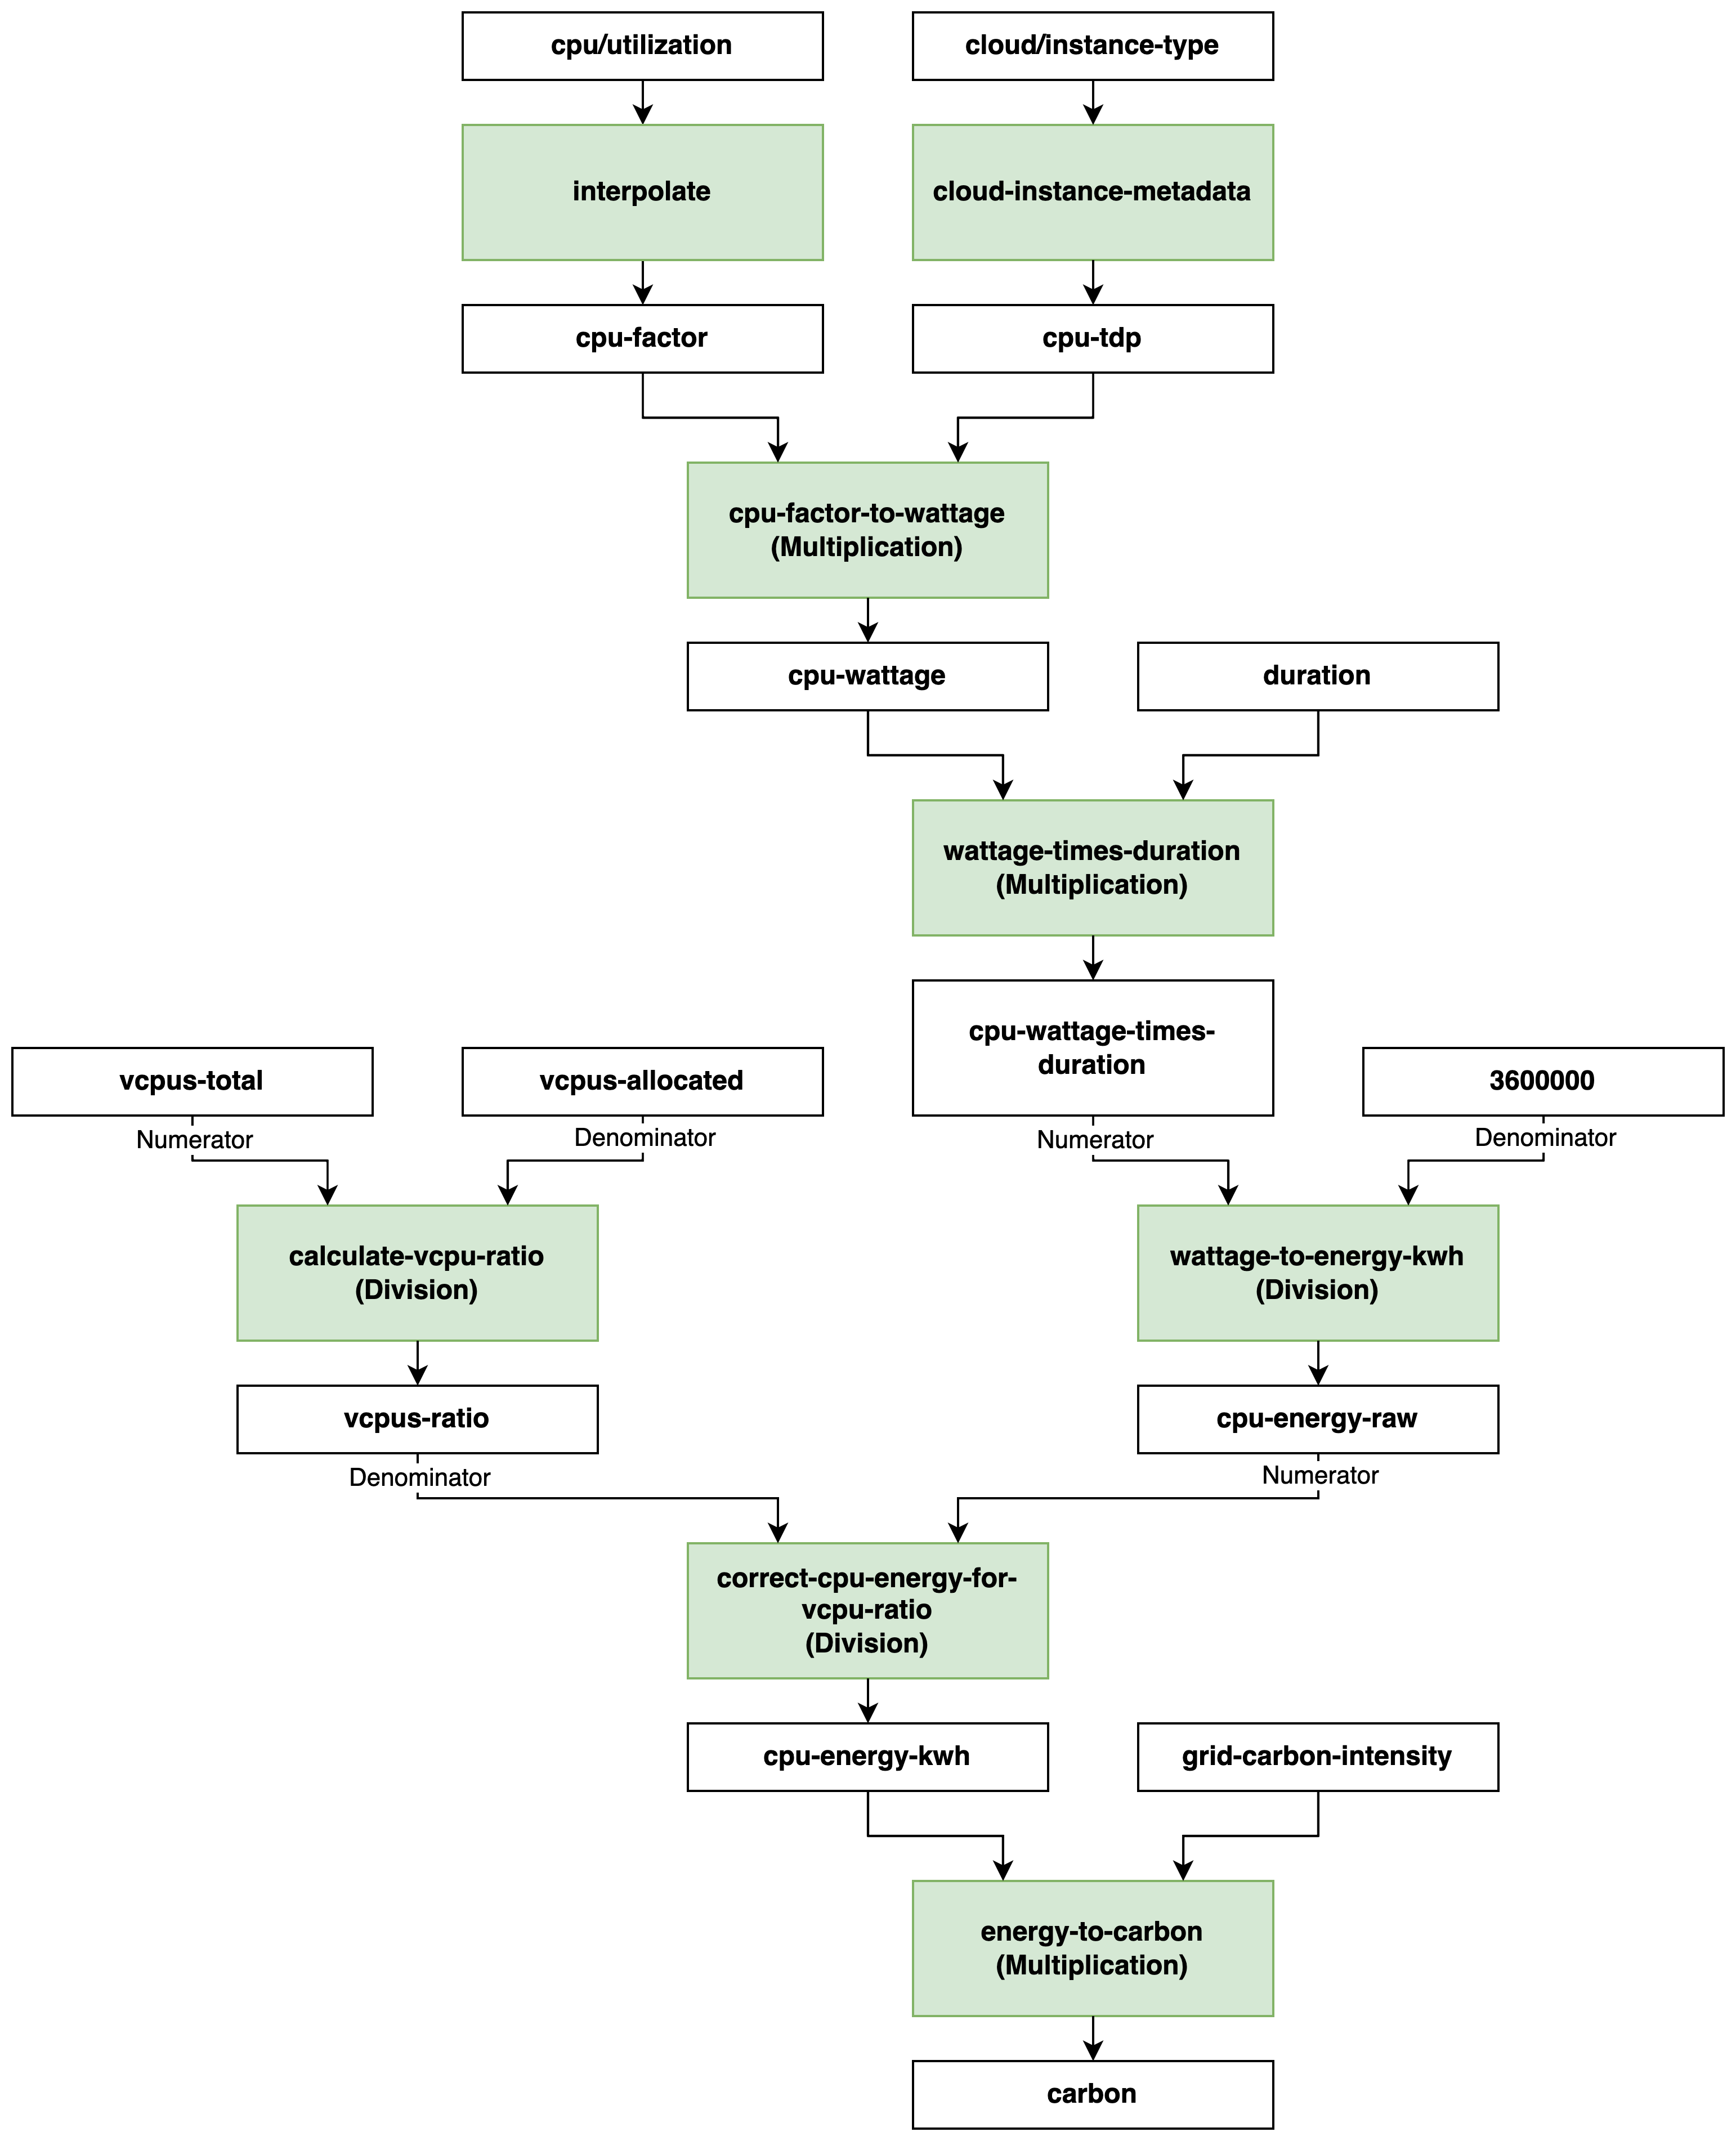
\includegraphics[width=1\linewidth]{images/impact_framework.png}
  \caption{Impact Framework pipeline to estimate carbon footprint of a cloud instance}
  \label{fig:impact_framework}
\end{figure}


\newpage

\section{End-to-End workflow}
\label{sec:e2eflow}

In this section we will provide a complete end-to-end workflow of the system, from the user request to the final provision of the workload.
First, we will describe the workflow in a high-level manner, and then we will provide a detailed sequence diagram (Figure \ref{fig:sequence_diagram}) that illustrates the interactions between the various components of the system.
We must note that the workflow described in this section is a simplified version of the actual system, as it does not include some low level details.

\begin{enumerate}
  \item User (Developer, Data Scientist, etc) selects the VmTemplate Composition card on the Krateo PlatformOps Portal (UI)
  \item User fills in the VmTemplate Composition form with the required fields (e.g., MinCPU, MinRAM, Deadline, Duration, MaxLatency)
  \item This triggers and Helm install of the VmTemplate Composition on the Cluster
  \item A VmTemplate Composition CREATE API request is sent to the Kubernetes API server
  \item Authentication and Authorization checks are performed by the Kubernetes API server
  \item The VmTemplate Composition CREATE API request is intercepted by a K8s Mutating Webhook configured with OPA as webhook server
  \item AdmissionReview request is sent to the OPA server
  \item OPA evaluates the AdmissionReview request against the policies
  \begin{enumerate}
    \item Cloud Provider is selected among the available providers
    \item Eligible regions are calculated based on the selected Cloud Provider and the MaxLatency parameter
    \item GDPR policy (if enabled) is evaluated and a subset of eligible regions is returned
    \item A scheduling request is sent to the GreenOps Scheduler along with the eligible regions and a set of parameters
    \item The GreenOps Scheduler returns a decision with the selected region and scheduling time
    \item OPA maps the return ElectricityMaps region name to the Cloud Provider region name
    \item OPA creates the JSON patch with the provider, schedulingRegion, and schedulingTime fields
    \item OPA crafts and sends the AdmissionReview response to the K8s API server 
  \end{enumerate}
  \item The K8s Mutating Webhook receives the AdmissionReview response and mutates the VmTemplate Composition specification
  \item K8s API server perform resource validation
  \item The VmTemplate Composition is persisted in the etcd database
  \item A periodic Helm upgrade operation is done by Krateo Composition Dynamic Controller
  \item After schedulingTime is reached, an Helm upgrade operation will install the provider-specific manifests for VM provisioning on the K8s Cluster
  \item Cloud provider Operator (e.g., Azure Operator) that is constantly watching for new provider-specific resources is triggered
  \item The Cloud provider Operator provisions the VM (and required resources) on the Cloud Provider
  \item The VM is up and running on the cloud
\end{enumerate}

\begin{sidewaysfigure}
  \centering
  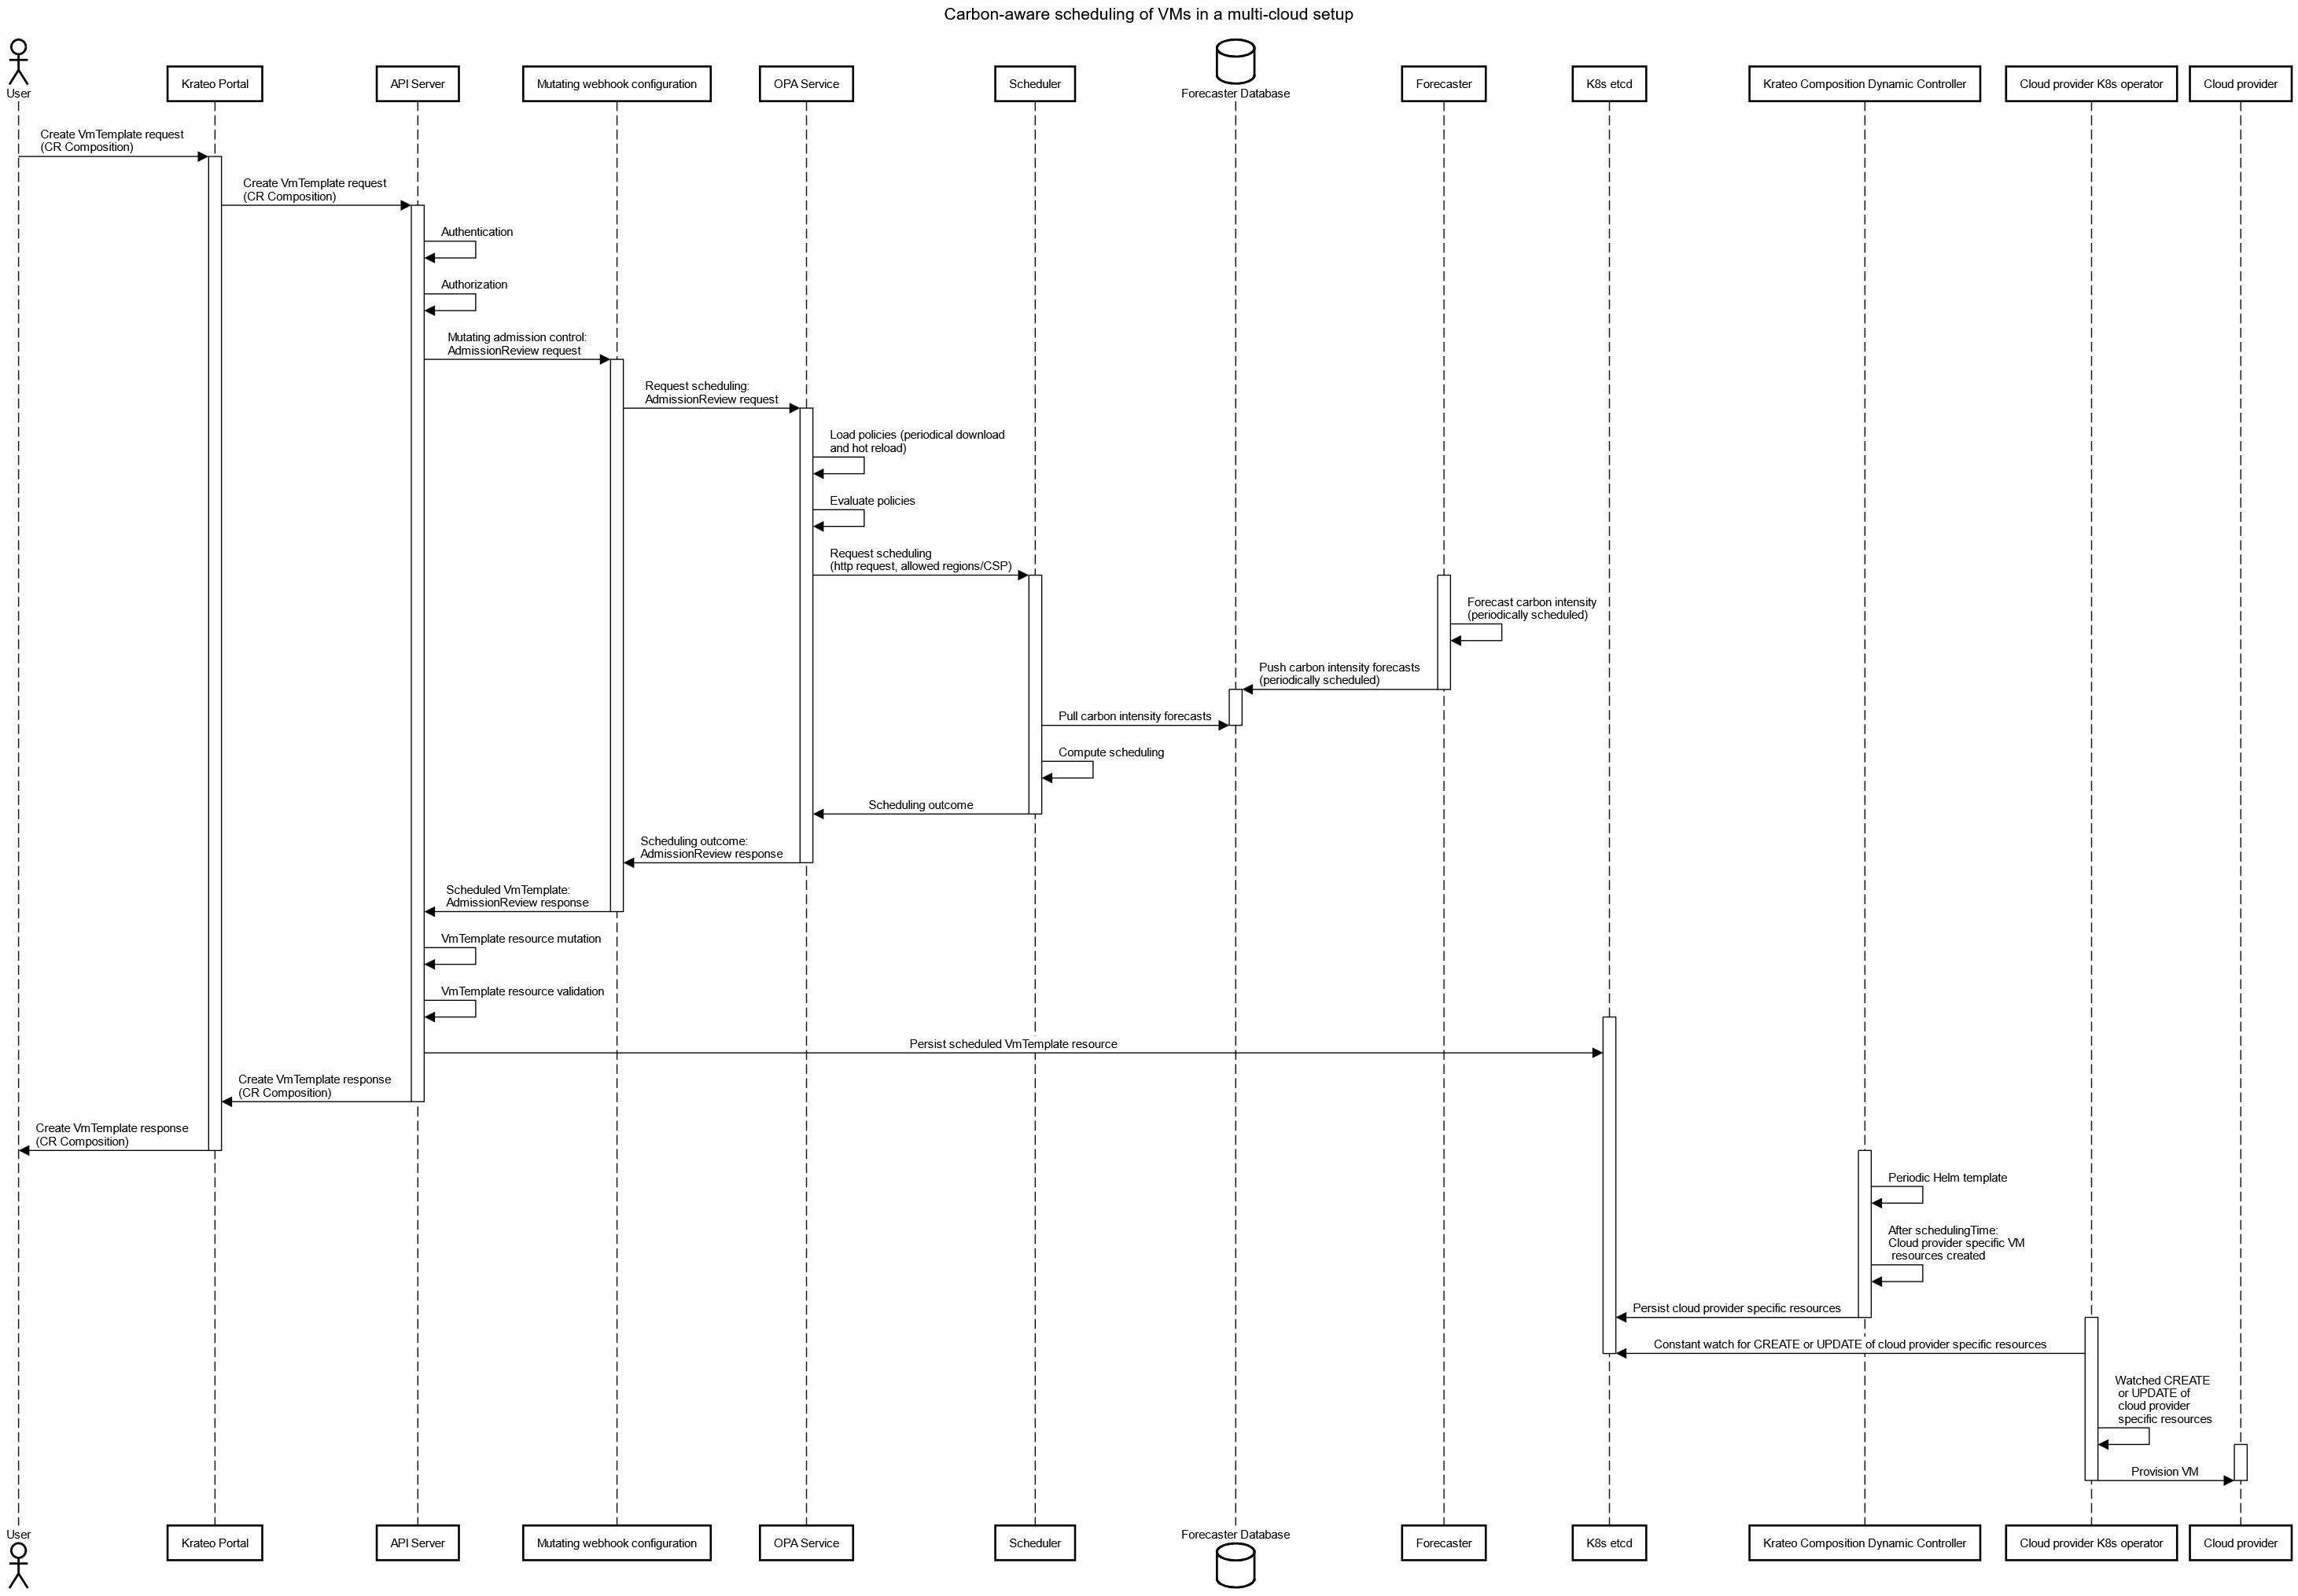
\includegraphics[width=\textheight]{images/sequence_diagram.png}
  \caption{Sequence diagram of the end-to-end workflow}
  \label{fig:sequence_diagram}
\end{sidewaysfigure}

\newpage
